\documentclass[11pt]{article}
\usepackage[margin=0.9in]{geometry}
\usepackage{amsmath,amssymb,amsthm}
\usepackage{booktabs,enumitem,multicol,xcolor,fancyhdr,longtable,array}
\usepackage[most]{tcolorbox}
\usepackage{listings}
\usepackage{pdflscape}
\usepackage{tikz}
\usetikzlibrary{arrows.meta,positioning,decorations.pathreplacing,calc}
\usepackage{pgfplots}
\usepgfplotslibrary{groupplots,fillbetween}
\pgfplotsset{compat=1.18}
\usepackage[hidelinks]{hyperref}

\definecolor{accent}{HTML}{1F4E79}
\definecolor{codebg}{HTML}{F5F5F5}
\definecolor{tipbg}{HTML}{FFF6DD}
\definecolor{exbg}{HTML}{EEF6EE}
\definecolor{dataclr}{HTML}{1F5C6B}
\definecolor{hsclr}{HTML}{D98A00}

\lstset{
  language=Python, basicstyle=\ttfamily\small, backgroundcolor=\color{codebg},
  keywordstyle=\color{accent}\bfseries, commentstyle=\color{gray}\itshape,
  frame=single, rulecolor=\color{gray!40}, columns=fullflexible,
  keepspaces=true, showstringspaces=false, aboveskip=6pt, belowskip=6pt,
  morekeywords={np}
}
\lstdefinestyle{output}{language={}, basicstyle=\ttfamily\scriptsize, backgroundcolor=\color{white},
  keywordstyle={}, commentstyle={}}

\newtcolorbox{keybox}[1][]{colback=accent!6, colframe=accent, boxrule=0.6pt,
  arc=2pt, left=6pt, right=6pt, top=4pt, bottom=4pt, fonttitle=\bfseries, #1}
\newtcolorbox{tipbox}[1][]{colback=tipbg, colframe=orange!70!black, boxrule=0.6pt,
  arc=2pt, left=6pt, right=6pt, top=4pt, bottom=4pt, fonttitle=\bfseries, #1}
\newtcolorbox{examplebox}[1][]{colback=exbg, colframe=green!40!black, boxrule=0.6pt,
  arc=2pt, left=6pt, right=6pt, top=4pt, bottom=4pt, fonttitle=\bfseries, breakable, #1}

\newcommand{\E}{\mathbb{E}}
\newcommand{\Var}{\operatorname{var}}
\newcommand{\Cov}{\operatorname{cov}}
\newcommand{\corr}{\operatorname{corr}}
\newcommand{\se}{\operatorname{se}}
\newcommand{\MSE}{\operatorname{MSE}}
\newcommand{\Bias}{\operatorname{Bias}}
\renewcommand{\P}{\mathbb{P}}
\newcommand{\given}{\mid}
\newcommand{\Bern}{\text{Bernoulli}}
\newcommand{\Bin}{\text{Binomial}}
\newcommand{\Norm}{\text{Normal}}
\newcommand{\SSR}{\mathrm{SSR}}
\newcommand{\SST}{\mathrm{SST}}
\newcommand{\py}[1]{\texttt{#1}}
\newcommand{\Ybar}{\overline{Y}}
\newcommand{\Xbar}{\overline{X}}
\newcommand{\inwords}[1]{\par\smallskip{\small\color{accent!80!black}\textit{In words:} #1}}
\newcommand{\why}[1]{&&\text{\small\color{gray}(#1)}}

\setlength{\parindent}{0pt}
\emergencystretch=3em
\setlength{\parskip}{5pt}
\setlength{\headheight}{14pt}
\pagestyle{fancy}
\fancyhf{}
\lhead{Math 50 -- Midterm 2 notes (Lectures 8--16, 10/2--10/21)}
\rhead{Unit 2.4, Unit 3, Unit 4}
\cfoot{\thepage}

\title{\textbf{Math 50 Midterm 2 Notes: Estimators, Uncertainty, and Regression}\\[2pt]
\large Lectures 8--16 (10/2--10/21) and the Unit 3--4 course notes}
\author{}
\date{}

\begin{document}
\maketitle
\thispagestyle{fancy}

\begin{tipbox}[title={How to use these notes}]
These notes combine the slides from 10/2, 10/5, 10/7, 10/9, 10/12, 10/14, 10/19 and 10/21 with the Unit 3 and Unit 4 course notes,
organized by topic instead of by lecture. Every derivation is written out step by step, with the reason for each step in gray on the right.

\textbf{New to the notation?} Start with the \hyperref[sec:glossary]{Glossary} right after the contents: every symbol, how to read it
aloud, what it means, and an example. Then read Section~\ref{sec:toolkit}, which reviews the Unit 1--2 rules (from Lectures 1--7) with a
small worked example for each. If a step later confuses you, the rule it needs is in Section~\ref{sec:toolkit}.

Green boxes are worked examples (most of them are the in-class questions, with solutions). Blue boxes are the results to remember; each
ends with an \emph{In words} line that reads the formula in plain English. The last page is a one-page formula sheet with a short symbol key.

The figures are \emph{illustrations} of the pictures in the slides, drawn from formulas or from made-up data; they are not the
real datasets. All code is Python, exactly as in the slides and notes.
\end{tipbox}

\tableofcontents

%==========================================================
\clearpage
\section*{Glossary of notation}\label{sec:glossary}
\addcontentsline{toc}{section}{Glossary of notation}
%==========================================================
Read the ``Read as'' column out loud: most of the confusion with math notation goes away once you can \emph{say} a formula.
Entries are grouped by topic; within each group the symbols appear roughly in the order you will meet them.

{\small
\setlength{\tabcolsep}{4pt}
\renewcommand{\arraystretch}{1.3}
\newcommand{\gh}[1]{\multicolumn{4}{@{}l}{\color{accent}\bfseries\normalsize #1}\\\midrule}
\begin{longtable}{@{}>{\raggedright\arraybackslash}p{2.5cm}>{\raggedright\arraybackslash}p{3.0cm}>{\raggedright\arraybackslash}p{5.5cm}>{\raggedright\arraybackslash}p{4.5cm}@{}}
\toprule
\textbf{Symbol} & \textbf{Read as} & \textbf{Meaning} & \textbf{Example}\\
\midrule
\endfirsthead
\toprule
\textbf{Symbol} & \textbf{Read as} & \textbf{Meaning} & \textbf{Example}\\
\midrule
\endhead
\bottomrule
\endfoot
\gh{A. General math}
$=$,\ $\approx$ & ``equals'', ``is approximately'' & exactly equal vs.\ close to & $\sqrt{42}\approx6.48$\\
$\propto$ & ``is proportional to'' & changes by the same factor & CI width $\propto1/\sqrt N$: 4$\times$ the data, half the width\\
$\Longrightarrow$ & ``implies'', ``so'' & the left side forces the right side & $\sqrt N\ge7.84\Longrightarrow N\ge61.5$\\
$\iff$ & ``if and only if'' & the two statements are equivalent (each implies the other) & $|\hat T|>1.96\iff$ the CI excludes 0\\
$\to$ & ``tends to'', ``approaches'' & gets closer and closer to & $\se(\Ybar)\to0$ as $N\to\infty$\\
$\infty$ & ``infinity'' & without limit; $N\to\infty$ means ``as we collect more and more data'' & \\
$\ge$,\ $\le$,\ $\gtrsim$ & ``at least'', ``at most'', ``roughly at least'' & comparisons & $N\gtrsim20$: about 20 or more\\
$\sum_{i=1}^N a_i$ & ``the sum from $i$ equals 1 to $N$ of $a$ sub $i$'' & $a_1+a_2+\cdots+a_N$. Plain $\sum_i$ means ``over all data points'' & $\sum_{i=1}^3 i=1+2+3=6$\\
$Y_i$ & ``$Y$ sub $i$'', ``$Y$ $i$'' & the $i$-th data point & $Y_3$ is the third observation\\
$X_{k,i}$ & ``$X$ sub $k$ comma $i$'' & value of predictor $k$ for data point $i$ & $X_{2,5}$: the IQ of mother 5, if predictor 2 is IQ\\
$Y_t$,\ $Y_{t-1}$ & ``$Y$ sub $t$'', ``$Y$ sub $t$ minus 1'' & value at time $t$; value one step earlier & today's and yesterday's log price\\
$\dots$,\ $\cdots$ & ``and so on'' & continue the obvious pattern & $Y_1,\dots,Y_N$ = all $N$ data points\\
$|x|$ & ``absolute value of $x$'' & size of $x$, ignoring its sign & $|-0.4|=0.4$\\
$\sqrt{x}$,\ $x^2$ & ``square root of $x$'', ``$x$ squared'' & & $\sqrt{3/2}\approx1.22$\\
$e^x$,\ $\ln x$,\ $\log_{10}x$ & ``$e$ to the $x$'', ``natural log'', ``log base 10'' & exponential function and its inverses & $e^x\approx1+x$ for small $x$\\
$\int_a^b f(y)\,dy$ & ``integral from $a$ to $b$ of $f$'' & area under the curve $f$ between $a$ and $b$ & $\P(a<Y<b)=\int_a^bf(y)\,dy$ (Lecture 4)\\
$\in$ & ``is in'', ``belongs to'' & membership in a set or interval & $y\in S$;\ \ $\rho\in[-1,1]$\\
$\{\dots\}$ & ``the set'' & a list of possible values & a die: $S=\{1,2,3,4,5,6\}$\\
$[a,b]$,\ $(a,b)$ & ``closed / open interval from $a$ to $b$'' & all numbers between $a$ and $b$, with / without the endpoints & a probability is in $[0,1]$\\
$\operatorname*{argmin}_b f(b)$ & ``the $b$ that minimizes $f$'' & the \emph{input} that gives the smallest output (not the smallest value itself) & least squares: $(\hat\beta_0,\hat\beta_1)$ is the argmin of SSR\\
$\square$ & ``end of proof'' & the argument is finished & \\
$'$ (prime) & ``prime'' & \textbf{two meanings}: $F'(y)$ is a derivative (Lecture 4); $\beta'$ is a single-predictor coefficient (Lectures 12--13) & $\beta'_{hs}=11.8$ vs.\ $\beta_{hs}=5.95$\\
\gh{B. Probability (Units 1--2)}
$Y$ vs.\ $y$ & ``capital $Y$'', ``little $y$'' & capital = random variable (not yet known); lowercase = one particular value it could take & $\P(Y=y)$: chance $Y$ comes out as $y$\\
$S$ & ``the sample space'' & every possible outcome & a coin: $S=\{0,1\}$\\
$E$,\ $\P(E)$ & ``event $E$'', ``probability of $E$'' & an event is a set of outcomes & $\P(Y\text{ even})=3/6=1/2$ for a die\\
$P_Y(y)$ & ``$P$ sub $Y$ of $y$'' & the distribution of $Y$: the probability of each outcome, $\P(Y=y)$ & fair die: $P_Y(y)=1/6$\\
$\P(x,y)$ & ``probability of $x$ and $y$'' & \textbf{joint}: both happen & $\P(C{=}1,G{=}M)=0.0021$\\
$\P(x\given y)$ & ``probability of $x$ given $y$'' & \textbf{conditional}: among the cases with $y$, the fraction with $x$ & $\P(\text{sad}\given\text{brown})=4/16=1/4$\\
$Y\given X$ & ``$Y$ given $X$'' & the distribution of $Y$ once $X$ is known & $Y\given X\sim\Norm(\beta_0+\beta_1X,\sigma_\epsilon^2)$\\
$\sim$ & ``is distributed as'', ``follows'' & names the distribution of a random variable & $Y\sim\Bern(0.75)$: a free throw\\
iid,\ $\overset{\text{iid}}{\sim}$ & ``independent and identically distributed'' & separate draws from the same distribution that do not affect each other & $N$ coin flips\\
$\Bern(q)$ & ``Bernoulli $q$'' & 0 or 1, with $\P(1)=q$ & made free throw, $q=0.75$\\
$\Bin(N,q)$ & ``Binomial $N$, $q$'' & number of 1's in $N$ iid $\Bern(q)$ & heads in 200 flips\\
$\text{Uniform}(a,b)$ & ``Uniform from $a$ to $b$'' & equally likely to land anywhere in $[a,b]$ & bus wait $T\sim\text{Uniform}(0,5)$\\
$\Norm(\mu,\sigma^2)$ & ``Normal with mean $\mu$, variance $\sigma^2$'' & the bell curve. The second number is the \emph{variance}, not the SD & $\Norm(0,1)$: the standard Normal\\
$f(y)$ & ``$f$ of $y$'', ``the density'' & height of the curve; probabilities are \emph{areas} under it & \\
$F(y)$ & ``$F$ of $y$'', ``the CDF'' & $\P(Y\le y)$: area to the left of $y$ & \\
$Z$,\ $\Phi(z)$ & ``$Z$'', ``capital phi of $z$'' & $Z\sim\Norm(0,1)$; $\Phi(z)=\P(Z<z)$ & $\Phi(1.96)\approx0.975$\\
$\mathbf 1_A$ & ``indicator of $A$'' & 1 if $A$ happens, 0 if not & $\E[\mathbf 1_A]=\P(A)$; \py{np.mean(x==2)}\\
$\E[Y]$ & ``expected value of $Y$'', ``E of $Y$'' & the long-run average, $\sum_y y\,P_Y(y)$ & a fair die: $3.5$\\
$\E[Y\given X]$ & ``expected $Y$ given $X$'' & average of $Y$ within the group with that value of $X$ & $\E[Y\given X{=}1]-\E[Y\given X{=}0]=\beta_1$\\
$\Var(Y)$,\ $\sigma^2$ & ``variance of $Y$'', ``sigma squared'' & average squared distance from the mean & $\Bern(q)$: $q(1-q)$\\
$\sigma$,\ $\sigma_Y$ & ``sigma (sub $Y$)'' & standard deviation $=\sqrt{\text{variance}}$; same units as $Y$ & test scores: $\sigma_Y=20.4$\\
$\Cov(X,Y)$ & ``covariance of $X$ and $Y$'' & do $X$ and $Y$ move together? $+$ together, $-$ opposite, $0$ no linear link & $\Cov(X,Y)=\beta_1\sigma_X^2$\\
$\rho$,\ $\corr(X,Y)$ & ``rho'', ``correlation'' & covariance rescaled to lie in $[-1,1]$ & $\hat\rho\approx0.45$ (mom's IQ, child's score)\\
$\rho_k$ & ``rho sub $k$'' & autocorrelation: correlation of values $k$ steps apart & AR(1): $\rho_k=\rho^k$\\
\gh{C. Greek letters}
$\mu$ & ``mew'' (mu) & a mean (true average) & $\E[Y]=\mu$\\
$\sigma$,\ $\Sigma$ & ``sigma'', ``capital sigma'' & $\sigma$: standard deviation; $\Sigma$: the sum sign, \textbf{or} (Unit 4.3--4.4) the covariance matrix of the predictors & $\Sigma=\begin{bmatrix}1&\rho\\\rho&1\end{bmatrix}$\\
$\rho$ & ``row'' (rho) & correlation & \\
$\beta$ & ``bay-tuh'' (beta) & regression coefficients & $\beta_0$ intercept, $\beta_1$ slope\\
$\epsilon$ & ``epsilon'' & noise: the part of $Y$ the line does not explain & $Y=\beta_0+\beta_1X+\epsilon$\\
$\theta$ & ``thay-tuh'' (theta) & a generic parameter, when the specific one does not matter & $\hat\theta$ estimates $\theta$\\
$\Phi$ & ``fye'' (capital phi) & the standard Normal CDF & \\
$\pi$ & ``pie'' & the number $3.14159\ldots$; appears in the Normal density & \\
$\lambda$ & ``lamb-duh'' (lambda) & a rate parameter (Lecture 4 only) & \\
\gh{D. Data, estimators, and regression}
$N$,\ $K$ & ``$N$'', ``$K$'' & number of data points (or length of a time series); number of predictors & $N=434$ children, $K=2$\\
$\hat\theta$ (hat) & ``theta hat'' & an \textbf{estimate} computed from data (random) of the true $\theta$ (fixed) & $\hat q=3/12$ estimates $q$\\
$\Ybar$ (bar) & ``$Y$ bar'' & sample average $\frac1N\sum_iY_i$ & $\Ybar$ of 2, 4, 6 is 4\\
$\se(\hat\theta)$ & ``standard error of theta hat'' & SD of the estimate over replicates of the data & $\se(\Ybar)=\sigma/\sqrt N$\\
$\MSE$,\ $\Bias$ & ``mean squared error'', ``bias'' & average squared miss; average miss $\E[\hat\theta]-\theta$ & $\MSE=\se^2+\Bias^2$\\
$\hat\sigma^2$,\ $\hat\sigma_0^2$ & ``sigma hat squared (sub zero)'' & variance estimates, dividing by $N-1$ / by $N$ & Bessel's correction\\
$S$,\ $\hat q_L$ & ``$S$'', ``$q$ hat sub $L$'' & number of 1's, $\sum_iY_i$; Laplace's estimate $\frac{S+1}{N+2}$ & two tails: $\hat q_L=1/4$, not $0$\\
CI & ``confidence interval'' & $\hat\theta\pm1.96\,\se(\hat\theta)$ & graders: $[-2,3]$\\
$H_0$ & ``H naught'', ``the null hypothesis'' & the claim we test, e.g.\ ``no effect'' & $H_0:\beta_1=0$\\
$\hat T$,\ $\hat T^*$ & ``T hat'', ``T star'' & test statistic from our data / from a replicate where $H_0$ is true & graders: $\hat T\approx0.4$\\
$p_v$ & ``p-value'' & $\P(|\hat T^*|>|\hat T|)$: how surprising our data would be if $H_0$ were true & graders: $0.69$\\
$\hat Y_i$,\ $r_i$ & ``$Y$ hat $i$'', ``residual $i$'' & fitted value $\hat\beta_0+\hat\beta_1X_i$; miss $Y_i-\hat Y_i$ & \\
SSR,\ SST & ``sum of squared residuals'', ``total sum of squares'' & $\sum_ir_i^2$; $\sum_i(Y_i-\Ybar)^2$ & \\
$S_{xx}$ & ``S x x'' & $\sum_i(X_i-\Xbar)^2\approx N\sigma_X^2$ & \\
$R^2$ & ``R squared'' & $1-\SSR/\SST$: fraction of the spread in $Y$ explained; estimates $\rho^2$ & test scores: $0.21$\\
$\beta_0$,\ $\beta_1$ & ``beta zero'', ``beta one'' & intercept and slope of the regression line & \\
$\beta_{hs}$,\ $\beta_{iq}$ & ``beta H S'', ``beta I Q'' & coefficient on the named predictor & $\hat\beta_{iq}=0.56$\\
$\beta'$ & ``beta prime'' & coefficient when that predictor is \emph{alone} in the model & $\hat\beta'_{hs}=11.8$\\
$\beta_{1,2}$ & ``beta one two'' & slope when $X_2$ is regressed on $X_1$ (the \emph{second} on the \emph{first}). The 10/21 slides write $\beta'_{1,j}$ for the same thing & $\beta_{hs,iq}=10.3$: IQ gap between the HS groups\\
$\sigma_\epsilon$ & ``sigma epsilon'' & SD of the noise: spread of points around the line & $\hat\sigma_\epsilon\approx5$ (graders)\\
categorical & & a predictor whose values are categories, not numbers on a scale & party of the incumbent; ethnicity\\
$X_{dem}$ (dummy) & ``X dem'' & dummy (indicator) variable: 1 if the data point is in that category, 0 if not & $X_{dem}=1$ for a Democratic incumbent\\
baseline & & the category left out (no dummy); every dummy coefficient is a difference from it & open seats; Black respondents\\
collinear & & predictors that are (almost) exact linear functions of each other & $X_{dem}+X_{rep}+X_{open}=1$; weight and hip size\\
$\rho_{1,2}$ & ``rho one two'' & correlation between the predictors $X_1$ and $X_2$ & past vote and inc: $0.86$\\
$R_j^2$ & ``R squared sub $j$'' & $R^2$ from regressing predictor $X_j$ on the \emph{other} predictors & weight on hip: $0.94^2=0.88$\\
\gh{E. Python}
\py{np.mean(x)}, \py{np.sum(x)}, \py{len(x)} & & average, total, count & \py{np.mean(x)} $=$ \py{np.sum(x)/len(x)}\\
\py{np.var(x)}, \py{np.std(x)} & & variance and SD (dividing by $N$) & \\
\py{np.cov(x,y)}\allowbreak\py{[0,1]} & & sample covariance (dividing by $N-1$); \py{[row, column]} counted from 0 & $\hat\beta_1$ = \py{C[0,1]/C[0,0]}\\
\py{y[x==0]} & & the $y$ values where $x$ is 0: data for ``$Y\given X=0$'' & \py{np.mean(y[x==0])}\\
\py{x**2} & & $x$ squared, element by element & \\
\py{Y[:-1]}, \py{Y[1:]} & & all but the last; all but the first & yesterday/today pairs\\
\py{np.random.}\allowbreak\py{binomial(N,q)} & & one $\Bin(N,q)$ draw & \\
\py{rng.normal(}\allowbreak\py{size=N)} & & $N$ draws from $\Norm(0,1)$ & \\
\py{norm.cdf(z)} & & $\Phi(z)$ (from \py{scipy.stats}) & \py{norm.cdf(1.96)} $\approx0.975$\\
\py{sm.OLS(y, X).fit()} & & least squares fit with statsmodels & Section~\ref{sec:mult}\\
\py{pd.get\_}\allowbreak\py{dummies(x)} & & one 0/1 column per category; \py{drop\_first=True} drops the first as the baseline & Section~\ref{sec:cat}\\
\end{longtable}
}

%==========================================================
\clearpage
\section{Toolkit: the probability and algebra used everywhere}\label{sec:toolkit}
%==========================================================
Almost every derivation in these notes uses only the facts below. They come from Units 1--2 (Lectures 1--7); each has a small worked
example from those lectures.

\subsection{Probability notation from Unit 1}
A \textbf{random variable} $Y$ is a quantity determined by chance (capital letter). It takes values in a \textbf{sample space} $S$; the
elements of $S$ are \textbf{outcomes}, and sets of outcomes are \textbf{events}. The \textbf{distribution} $P_Y(y)=\P(Y=y)$ gives the
probability of each outcome; these are $\ge0$ and add up to 1. We name distributions with $\sim$: $Y\sim\Bern(q)$ means
$S=\{0,1\}$ and $P_Y(1)=q$.

For two variables we use three kinds of probability:
\begin{itemize}[leftmargin=*,itemsep=2pt]
\item \textbf{Joint} $\P(x,y)$: both happen.
\item \textbf{Marginal} $\P(x)=\sum_y\P(x,y)$: ``sum out'' the variable you do not care about.
\item \textbf{Conditional} $\P(x\given y)=\dfrac{\P(x,y)}{\P(y)}$: among the cases where $y$ happened, the fraction where $x$ also happened.
\end{itemize}
$X$ and $Y$ are \textbf{independent} if $\P(x,y)=\P(x)\P(y)$ for \emph{every} pair $(x,y)$; equivalently, knowing one does not change the
probabilities of the other.

\begin{examplebox}[title={Examples (Lectures 1--2)}]
\textbf{A die.} $S=\{1,\dots,6\}$, $P_Y(y)=1/6$. The event ``$Y$ even'' is $\{2,4,6\}$, so $\P(Y\text{ even})=3/6=1/2$.

\textbf{Cancer diagnosis ($C$) and gender ($G$).} The joint table:
\begin{center}
\begin{tabular}{lccc}
\toprule
$\P(C,G)$ & $G=M$ & $G=F$ & sum\\\midrule
$C=1$ (diagnosed) & 0.0021 & 0.0019 & 0.0040\\
$C=0$ & 0.4899 & 0.5061 & 0.9960\\\midrule
sum & 0.4920 & 0.5080 & 1\\
\bottomrule
\end{tabular}
\end{center}
\emph{Marginal:} $\P(C=1)=0.0021+0.0019=0.004$ (sum across the row). \emph{Conditional:}
$\P(C=1\given G=M)=0.0021/0.492=0.00427$ (restrict to the $M$ column, then divide by its total).
\emph{Independent?} Compare one cell with the product of its margins: $\P(C{=}1)\P(G{=}M)=0.004\times0.492=0.00197\ne0.0021$, so not exactly.

\textbf{Eye color and mood.} Of 24 people, 16 have brown eyes and 4 of those are sad, so $\P(\text{sad}\given\text{brown})=4/16=1/4$,
while the joint probability is $\P(\text{sad},\text{brown})=4/24=1/6$. Conditioning shrinks the denominator to the group you condition on.
\end{examplebox}

\subsection{Sums ($\Sigma$ notation)}
$\sum_{i=1}^N a_i$ means $a_1+a_2+\cdots+a_N$. We often write just $\sum_i$. Three rules:
\begin{align*}
\sum_i c\,a_i &= c\sum_i a_i \why{a constant $c$ comes out of the sum}\\
\sum_i (a_i+b_i) &= \sum_i a_i+\sum_i b_i \why{a sum splits}\\
\sum_{i=1}^N c &= Nc \why{adding the same number $N$ times}
\end{align*}
The \textbf{sample average} is $\Ybar=\frac1N\sum_i Y_i$, so $\sum_i Y_i=N\Ybar$. An important consequence: deviations from the
sample average always sum to zero,
\[
\sum_i (Y_i-\Ybar)=\sum_i Y_i-N\Ybar=N\Ybar-N\Ybar=0 .
\]
Because of this, for any constant $c$ (including $c=\Xbar$ or $c=\Ybar$), $\sum_i c\,(Y_i-\Ybar)=c\cdot 0=0$. We will use this trick
several times.

\begin{examplebox}[title={Example}]
Data $Y_1,Y_2,Y_3=2,4,6$. Then $\sum_iY_i=12$, $\Ybar=12/3=4$, and the deviations $Y_i-\Ybar$ are $-2,0,2$, which sum to $0$.
Rule 1: $\sum_i 5Y_i=10+20+30=60=5\times12$. Rule 3: $\sum_{i=1}^3 7=21=3\times7$.
In Python (Lecture 3), \py{np.mean(x)} is exactly \py{np.sum(x) / len(x)}.
\end{examplebox}

\subsection{Expectation and variance}
The \textbf{expectation} (true mean) is the probability-weighted average of the outcomes,
$\E[Y]=\sum_y y\,P_Y(y)$ (for a density, $\E[Y]=\int y\,f(y)\,dy$), and more generally $\E[h(Y)]=\sum_y h(y)P_Y(y)$.
It is what the sample average approaches as $N$ grows: in an iid sample, the fraction of times outcome $y$ appears approaches $P_Y(y)$, with
an error proportional to $1/\sqrt N$ (Lecture 3; Section~\ref{sec:clt} makes this precise).
\begin{itemize}[leftmargin=*,itemsep=2pt]
\item \textbf{Linearity:} $\E[aX+bY+c]=a\E[X]+b\E[Y]+c$ for any random variables (independent or not). $\E[c]=c$ for a constant.
\item \textbf{Indicators:} a probability is the expectation of a 0/1 variable: $\E[\mathbf 1_A]=\P(A)$. That is why \py{np.mean(x == 2)}
estimates $\P(X=2)$.
\item \textbf{Variance:} $\Var(X)=\E[(X-\E X)^2]=\E[X^2]-(\E X)^2$, and $\sigma_X=\sqrt{\Var X}$.
\item \textbf{Shifting and scaling:} $\Var(aX+b)=a^2\Var(X)$. Adding a constant does not change the spread; multiplying by $a$
multiplies the spread by $|a|$ and the variance by $a^2$.
\item \textbf{Independent sums:} if $X,Y$ are independent, $\Var(X+Y)=\Var X+\Var Y$ and $\E[XY]=\E[X]\E[Y]$.
Note $\Var(X-Y)=\Var X+\Var Y$ too (since $\Var(-Y)=(-1)^2\Var Y$).
\end{itemize}

\begin{examplebox}[title={Examples (Lectures 5--6)}]
\textbf{A three-valued variable.} $\P(Y{=}1)=\tfrac12$, $\P(Y{=}2)=\tfrac13$, $\P(Y{=}3)=\tfrac16$. Then
\[
\E[Y]=1\cdot\tfrac12+2\cdot\tfrac13+3\cdot\tfrac16=\tfrac53,\qquad
\E[Y^2]=1\cdot\tfrac12+4\cdot\tfrac13+9\cdot\tfrac16=\tfrac{10}3,\qquad
\Var(Y)=\tfrac{10}3-\big(\tfrac53\big)^2=\tfrac{30}{9}-\tfrac{25}{9}=\tfrac59 .
\]
Note $\E[Y^2]$ means ``square first, then average'' ($\tfrac{10}{3}$), which is not $(\E Y)^2$ ($\tfrac{25}{9}$).

\textbf{Bernoulli variance.} $Y\sim\Bern(q)$: $\E[Y]=0\cdot(1-q)+1\cdot q=q$. Since $Y$ is 0 or 1, $Y^2=Y$, so $\E[Y^2]=q$ and
$\Var(Y)=q-q^2=q(1-q)$. It is largest ($\tfrac14$) at $q=\tfrac12$ and zero at $q=0$ or $1$ (no randomness).
\end{examplebox}

\begin{keybox}[title={The variance of a sample average}]
If $Y_1,\dots,Y_N$ are iid (independent, identically distributed) with mean $\mu$ and variance $\sigma^2$, then
\begin{align*}
\E[\Ybar]&=\tfrac1N\textstyle\sum_i\E[Y_i]=\tfrac1N\cdot N\mu=\mu, \\
\Var(\Ybar)&=\Var\!\Big(\tfrac1N\textstyle\sum_iY_i\Big)=\tfrac{1}{N^2}\Var\!\Big(\textstyle\sum_iY_i\Big)=\tfrac{1}{N^2}\cdot N\sigma^2=\dfrac{\sigma^2}{N}.
\end{align*}
The step $\Var(\sum_iY_i)=N\sigma^2$ uses independence. So the standard deviation of $\Ybar$ is $\sigma/\sqrt N$: four times the data
halves the spread.
\inwords{averaging $N$ independent measurements keeps the center at the true mean and divides the variance by $N$, so the typical
error of an average shrinks like $1/\sqrt N$.}
\end{keybox}

\subsection{Conditioning: what $Y\given X$ and ``conditional on $X$'' mean}
\textbf{$Y\given X$} (``$Y$ given $X$'') is the distribution of $Y$ once we know the value of $X$. Regression models are written this way:
we say how $X$ is drawn, then how $Y$ is drawn \emph{for each value} of $X$. Lecture 2's example, coding $G=1$ for male:
\[
C\given G\sim\Bern\big(q_1G+q_0(1-G)\big),
\]
with $q_1=\P(C{=}1\given G{=}1)=0.00427$ and $q_0=\P(C{=}1\given G{=}0)=0.00374$.
When $G=1$ the success probability is $q_1$; when $G=0$ it is $q_0$. The difference $q_1-q_0=0.00053$ is the ``effect'' of being male.

\textbf{$\E[Y\given X]$} (``expected $Y$ given $X$'') is the average of $Y$ within the group that has that value of $X$. In data:
\py{np.mean(y[x == 1])}. It depends on $X$, so it is itself a random variable.

\textbf{Tower property:} $\E\big[\E[Y\given X]\big]=\E[Y]$: average the group averages, weighting each group by how likely it is.

\begin{examplebox}[title={Example (Lecture 5): the tower property}]
$X\sim\Bern(\tfrac12)$ and $Y\in\{1,2,3\}$ with $\P(Y\given X{=}0)=(\tfrac12,\tfrac14,\tfrac14)$ and $\P(Y\given X{=}1)=(\tfrac13,\tfrac13,\tfrac13)$. Then
\[
\E[Y\given X{=}0]=1\cdot\tfrac12+2\cdot\tfrac14+3\cdot\tfrac14=\tfrac74,\qquad \E[Y\given X{=}1]=\tfrac{1+2+3}{3}=2,
\]
\[
\E[Y]=\tfrac12\cdot\tfrac74+\tfrac12\cdot2=\tfrac{15}{8},\qquad
\E[XY]=\P(X{=}1)\cdot\E[Y\given X{=}1]=\tfrac12\cdot2=1
\]
(when $X=0$ the product $XY$ is $0$, so only the $X=1$ group contributes).
\end{examplebox}

\textbf{``Conditional on $X_1,\dots,X_N$''} (used from Section~\ref{sec:ls} on) means: treat the $X$ values in the dataset as fixed
numbers, and imagine redrawing only the $Y$'s. In the graders example, it means keeping the same assignment of exams to graders and asking
how the scores could have come out differently.

\subsection{Covariance and correlation}
$\Cov(X,Y)=\E\big[(X-\E X)(Y-\E Y)\big]$: positive if $X$ and $Y$ tend to be above their means together, negative if one tends to be above
when the other is below. Expanding the product and using linearity (this exact computation is on the 10/7 slides):
\begin{align*}
\E\big[(X-\E X)(Y-\E Y)\big]&=\E\big[XY-\E[Y]X-\E[X]Y+\E[X]\E[Y]\big] \why{expand}\\
&=\E[XY]-\E[Y]\E[X]-\E[X]\E[Y]+\E[X]\E[Y] \why{linearity ($\E X,\E Y$ constants)}\\
&=\E[XY]-\E[X]\E[Y].
\end{align*}
Rules you will need:
\begin{itemize}[leftmargin=*,itemsep=2pt]
\item $\Cov(X,X)=\Var(X)$ and $\Cov(X,Y)=\Cov(Y,X)$.
\item \textbf{Bilinearity:} $\Cov(X,\,aY+bZ+c)=a\Cov(X,Y)+b\Cov(X,Z)$. Constants drop out; coefficients come out.
\item If $X,Y$ are independent then $\Cov(X,Y)=0$ (because $\E[XY]=\E X\E Y$). The converse is false.
\item In general $\Var(X+Y)=\Var X+\Var Y+2\Cov(X,Y)$.
\item \textbf{Correlation:} $\rho=\corr(X,Y)=\dfrac{\Cov(X,Y)}{\sigma_X\sigma_Y}$; it has no units and lies in $[-1,1]$.
\end{itemize}

\begin{examplebox}[title={Example (Lecture 7): reading covariance off a plot}]
$X\sim\Bern(\tfrac12)$ and the plot shows group means $\E[Y\given X{=}0]\approx2$, $\E[Y\given X{=}1]\approx6$, with spread $\sigma_\epsilon\approx1$
in each group. The slope is the difference of group means, $\beta_1\approx6-2=4$. Since $\sigma_X^2=\tfrac12\cdot\tfrac12=\tfrac14$,
\[
\Cov(X,Y)=\beta_1\sigma_X^2\approx4\cdot\tfrac14=1,\qquad
\sigma_Y^2=\beta_1^2\sigma_X^2+\sigma_\epsilon^2\approx16\cdot\tfrac14+1=5 .
\]
(The first formula is proved in Section~\ref{sec:regmodel}; the second in Section 2.)
\end{examplebox}

\subsection{Normal, Bernoulli, Binomial}
\begin{itemize}[leftmargin=*,itemsep=2pt]
\item $X\sim\Norm(\mu,\sigma^2)$: the second number is the \emph{variance}. $aX+b\sim\Norm(a\mu+b,a^2\sigma^2)$, and a sum of
independent Normals is Normal (means add, variances add).
\item \textbf{Standardizing:} $Z=(X-\mu)/\sigma\sim\Norm(0,1)$. We write $\Phi(z)=\P(Z<z)$ for the standard Normal CDF.
\item About $68\%$, $95\%$, $99.7\%$ of a Normal lies within $1,2,3$ standard deviations of the mean. More precisely, $95\%$ lies
within $\pm1.96\,\sigma$; this $1.96$ shows up in every confidence interval.
\item $Y\sim\Bern(q)$: $\E Y=q$, $\Var Y=q(1-q)$. $S=\sum_{i=1}^NY_i\sim\Bin(N,q)$: $\E S=Nq$, $\Var S=Nq(1-q)$.
\end{itemize}

\begin{examplebox}[title={Example: using the 68\% rule}]
Heights $Y\sim\Norm(64,\ 2.5^2)$ (inches). What fraction are taller than $66.5$? Standardize: $z=(66.5-64)/2.5=1$, so we need
$\P(Z>1)$. $68\%$ lies within one SD, so $32\%$ lies outside, split equally between the two tails by symmetry: $\P(Z>1)\approx16\%$
(equivalently $\Phi(1)\approx0.84$, Lecture 6).
\end{examplebox}

\subsection{The single-predictor regression model (from Unit 2)}\label{sec:regmodel}
\[
Y\given X\sim\Norm(\beta_0+\beta_1X,\ \sigma_\epsilon^2)\qquad\Longleftrightarrow\qquad Y=\beta_0+\beta_1X+\epsilon,\quad \epsilon\sim\Norm(0,\sigma_\epsilon^2),
\]
with $\epsilon$ independent of $X$. Read it as ``to make a $Y$, take the line's height at $X$ and add Normal noise.'' The model assumes
(1) $Y\given X$ is Normal, (2) the conditional mean is a line, $\E[Y\given X=x]=\beta_0+\beta_1x$, and (3) the spread $\Var(Y\given X)=\sigma_\epsilon^2$
is the same for every $x$. Key facts from Unit 2:
\[
\E[Y]=\beta_0+\beta_1\E[X],\qquad \Cov(X,Y)=\beta_1\sigma_X^2\ \Longrightarrow\ \beta_1=\frac{\Cov(X,Y)}{\sigma_X^2}.
\]
(Proof of the second: $\Cov(X,Y)=\Cov(X,\beta_0+\beta_1X+\epsilon)=\beta_1\Cov(X,X)+\Cov(X,\epsilon)=\beta_1\sigma_X^2+0$.)

\begin{examplebox}[title={Example (Lecture 7): from code to a model to a number}]
\begin{lstlisting}
n = 100000
x = np.random.uniform(0, 2, n)
y = np.zeros(n)
for i in range(n):
    y[i] = np.random.normal(2 + 3*x[i], 1)
print(np.var(y))
\end{lstlisting}
\textbf{Model:} $X\sim\text{Uniform}(0,2)$, $\ Y\given X\sim\Norm(2+3X,\ 1)$ (\py{np.random.normal} takes the SD, here $1$).
\textbf{What prints?} $Y=2+3X+\epsilon$ with $\epsilon$ independent of $X$, so the variances add:
$\Var(Y)=3^2\Var(X)+1$. A $\text{Uniform}(a,b)$ has variance $(b-a)^2/12$, so $\Var(X)=4/12=\tfrac13$ and $\Var(Y)=9\cdot\tfrac13+1=4$.
\end{examplebox}

%==========================================================
\section{Correlation and the coefficient of determination (Unit 2.4)}
%==========================================================
\subsection{Correlation is the slope between standardized variables}
Let $X$ and $Y$ follow the regression model above and standardize both: $Z_X=(X-\mu_X)/\sigma_X$, $Z_Y=(Y-\mu_Y)/\sigma_Y$.
Each standardized variable has mean $0$ and standard deviation $1$, so it is ``in units of its own standard deviation.''
\textbf{Question:} what is the regression coefficient of $Z_Y$ on $Z_X$? Using $Y=\beta_0+\beta_1X+\epsilon$ and $\mu_Y=\beta_0+\beta_1\mu_X$:
\begin{align*}
Z_Y=\frac{Y-\mu_Y}{\sigma_Y}
&=\frac{(\beta_0+\beta_1X+\epsilon)-(\beta_0+\beta_1\mu_X)}{\sigma_Y} \why{substitute $Y$ and $\mu_Y$}\\
&=\frac{\beta_1(X-\mu_X)+\epsilon}{\sigma_Y} \why{$\beta_0$ cancels; factor out $\beta_1$}\\
&=\frac{\beta_1\sigma_X}{\sigma_Y}\cdot\frac{X-\mu_X}{\sigma_X}+\frac{\epsilon}{\sigma_Y} \why{multiply and divide by $\sigma_X$}\\
&=\frac{\beta_1\sigma_X}{\sigma_Y}\,Z_X+\frac{\epsilon}{\sigma_Y}. \why{definition of $Z_X$}
\end{align*}
This is again a regression model (no intercept, noise $\epsilon/\sigma_Y$), with slope $\beta_1\sigma_X/\sigma_Y$. Plugging in
$\beta_1=\Cov(X,Y)/\sigma_X^2$:
\begin{keybox}[title={Correlation}]
\[
\rho=\frac{\beta_1\sigma_X}{\sigma_Y}=\frac{\Cov(X,Y)}{\sigma_X\sigma_Y}.
\]
$\rho$ is the slope after both variables are measured in standard deviations: if $X$ is one SD above its mean, we expect $Y$ to be
$\rho$ SDs above its mean. Since $|\rho|\le 1$, the prediction is always less extreme than $X$ in SD units; this is
\emph{regression to the mean}.
\inwords{correlation is the covariance with the units taken out (divide by both standard deviations); it is the slope you get after measuring $X$ and $Y$ in standard deviations.}
\end{keybox}

\subsection{The coefficient of determination $\rho^2$}
Take the variance of both sides of $Y=\beta_0+\beta_1X+\epsilon$ ($X$ and $\epsilon$ are independent, so their variances add):
\begin{align*}
\sigma_Y^2&=\beta_1^2\sigma_X^2+\sigma_\epsilon^2 \why{variance of $Y=\beta_0+\beta_1X+\epsilon$}\\
1&=\frac{\beta_1^2\sigma_X^2}{\sigma_Y^2}+\frac{\sigma_\epsilon^2}{\sigma_Y^2} \why{divide by $\sigma_Y^2$}\\
1&=\rho^2+\frac{\sigma_\epsilon^2}{\sigma_Y^2}. \why{$\rho=\beta_1\sigma_X/\sigma_Y$}
\end{align*}
\begin{keybox}[title={Coefficient of determination}]
\[
1-\rho^2=\frac{\sigma_\epsilon^2}{\sigma_Y^2}=\frac{\Var(Y\given X)}{\Var(Y)},\qquad\text{equivalently}\qquad \rho^2=1-\frac{\sigma_\epsilon^2}{\sigma_Y^2}.
\]
$\rho^2$ is the \emph{fraction of the variance of $Y$ explained by $X$}. The total variance splits into an explained part
$\beta_1^2\sigma_X^2$ (moving along the line) and an unexplained part $\sigma_\epsilon^2$ (scatter around the line).
Since both parts are $\ge0$, $0\le\rho^2\le1$, which is why $-1\le\rho\le1$.
\inwords{$1-\rho^2$ is the share of $Y$'s variance left over after accounting for $X$, so $\rho^2$ is the share $X$ explains.}
\end{keybox}

\begin{figure}[h]
\centering
\pgfmathsetseed{4}
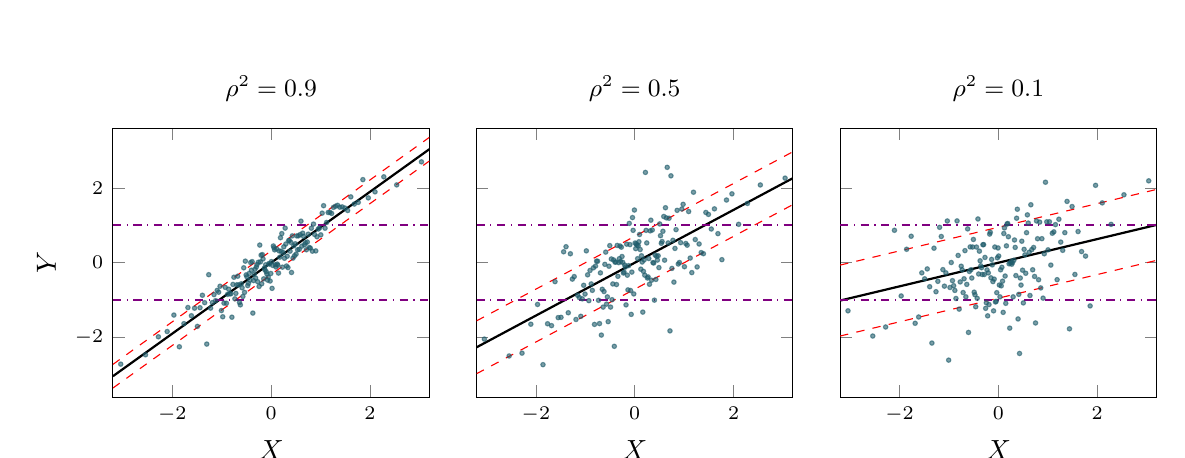
\begin{tikzpicture}
\begin{groupplot}[group style={group size=3 by 1, horizontal sep=0.6cm, y descriptions at=edge left},
  width=5.6cm, height=5cm, xmin=-3.2, xmax=3.2, ymin=-3.6, ymax=3.6, xlabel={$X$}, ylabel={$Y$},
  tick label style={font=\scriptsize}, title style={font=\small}]
\nextgroupplot[title={$\rho^2=0.9$}]
\addplot[only marks, mark size=0.8pt, dataclr, opacity=0.6, domain=0.004:0.996, samples=170]
  ({0.5513*ln(x/(1-x))},{0.9487*0.5513*ln(x/(1-x))+0.3162*sqrt(-2*ln(0.002+0.996*rnd))*cos(360*rnd)});
\addplot[black, thick, domain=-3.2:3.2] {0.9487*x};
\addplot[red, dashed, domain=-3.2:3.2] {0.9487*x+0.3162};
\addplot[red, dashed, domain=-3.2:3.2] {0.9487*x-0.3162};
\addplot[violet, dashdotted, thick, domain=-3.2:3.2] {1};
\addplot[violet, dashdotted, thick, domain=-3.2:3.2] {-1};
\nextgroupplot[title={$\rho^2=0.5$}]
\addplot[only marks, mark size=0.8pt, dataclr, opacity=0.6, domain=0.004:0.996, samples=170]
  ({0.5513*ln(x/(1-x))},{0.7071*0.5513*ln(x/(1-x))+0.7071*sqrt(-2*ln(0.002+0.996*rnd))*cos(360*rnd)});
\addplot[black, thick, domain=-3.2:3.2] {0.7071*x};
\addplot[red, dashed, domain=-3.2:3.2] {0.7071*x+0.7071};
\addplot[red, dashed, domain=-3.2:3.2] {0.7071*x-0.7071};
\addplot[violet, dashdotted, thick, domain=-3.2:3.2] {1};
\addplot[violet, dashdotted, thick, domain=-3.2:3.2] {-1};
\nextgroupplot[title={$\rho^2=0.1$}]
\addplot[only marks, mark size=0.8pt, dataclr, opacity=0.6, domain=0.004:0.996, samples=170]
  ({0.5513*ln(x/(1-x))},{0.3162*0.5513*ln(x/(1-x))+0.9487*sqrt(-2*ln(0.002+0.996*rnd))*cos(360*rnd)});
\addplot[black, thick, domain=-3.2:3.2] {0.3162*x};
\addplot[red, dashed, domain=-3.2:3.2] {0.3162*x+0.9487};
\addplot[red, dashed, domain=-3.2:3.2] {0.3162*x-0.9487};
\addplot[violet, dashdotted, thick, domain=-3.2:3.2] {1};
\addplot[violet, dashdotted, thick, domain=-3.2:3.2] {-1};
\end{groupplot}
\end{tikzpicture}
\caption{Simulated data with $\mu_X=\mu_Y=0$, $\sigma_X=\sigma_Y=1$, so $\beta_1=\rho$. Black: $\E[Y\given X]=\rho X$.
Red dashed: $\pm\sigma_\epsilon=\pm\sqrt{1-\rho^2}$ around the line. Purple: $\pm\sigma_Y=\pm1$. When $\rho^2$ is large, the scatter
around the line (red) is much narrower than the total scatter (purple); when $\rho^2$ is small they are almost the same width.}
\end{figure}

\begin{center}
\renewcommand{\arraystretch}{1.5}
\begin{tabular}{@{}llll@{}}
\toprule
 & Formula & Units & Range\\
\midrule
$\Cov(X,Y)$ & $\E[XY]-\E X\E Y$ & units $Y\times$ units $X$ & $(-\infty,\infty)$\\
$\beta_1$ & $\Cov(X,Y)/\sigma_X^2$ & units $Y$ / units $X$ & $(-\infty,\infty)$\\
$\rho$ & $\Cov(X,Y)/(\sigma_X\sigma_Y)$ & none & $[-1,1]$\\
$\rho^2$ & $1-\sigma_\epsilon^2/\sigma_Y^2$ & none & $[0,1]$\\
\bottomrule
\end{tabular}

{\small Summary: measures of association (10/2 slides). Only $\rho$ and $\rho^2$ can be compared across datasets with different units.}
\end{center}

%==========================================================
\section{The Law of Large Numbers and the Central Limit Theorem (Unit 3.1)}\label{sec:clt}
%==========================================================
These two theorems explain \emph{why} sample averages work and why Normal distributions show up everywhere in this unit.

\begin{keybox}[title={Law of Large Numbers (LLN)}]
If $X_1,\dots,X_N$ are iid with $\E[X_i]<\infty$ and $S_N=\sum_{i=1}^NX_i$, then $S_N/N\to\E[X_i]$ as $N\to\infty$.
\inwords{with enough independent data, the sample average lands close to the true mean.}
\end{keybox}
In words: for large $N$ the sample average will not differ from the true mean by much. The toolkit tells us \emph{how} much:
$\Var(S_N/N)=\sigma^2/N$, so the typical error shrinks like $1/\sqrt N$. That calculation never used the shape of the
distribution, only its variance, which hints that something universal is going on.

\begin{keybox}[title={Central Limit Theorem (CLT)}]
If $X_1,\dots,X_N$ are iid with $\E[X_i]=\mu$, $\Var(X_i)=\sigma^2$, and $S_N=\sum_iX_i$, then
\[
\P\!\left(\frac{S_N-N\mu}{\sqrt{N\sigma^2}}<z\right)\to\P(Z<z)=\Phi(z),\qquad Z\sim\Norm(0,1).
\]
Informally: $S_N\approx\Norm(N\mu,\ N\sigma^2)$, and dividing by $N$, $\ \Ybar\approx\Norm(\mu,\ \sigma^2/N)$, \emph{whatever} the
distribution of the $X_i$ (as long as the variance is finite).
\inwords{add up (or average) many independent pieces and the result follows a bell curve, whatever shape each piece has.}
\end{keybox}
The fraction $(S_N-N\mu)/\sqrt{N\sigma^2}$ is just $S_N$ standardized: subtract its mean $N\mu$, divide by its standard deviation
$\sqrt{N\sigma^2}$.

\textbf{The iid assumption matters.} The CLT above needs independent, identically distributed pieces. Strong correlation between the
$X_i$ (as in the time series of Section~\ref{sec:ar}) can change the sample distribution a lot, so check that iid is reasonable first.

\begin{examplebox}[title={Example: Binomial approximation (drill from the notes)}]
$Y\sim\Bin(200,0.3)$, i.e.\ $Y$ is a sum of $N=200$ iid $\Bern(0.3)$ variables. Estimate $\P(Y<70)$.

Each Bernoulli has $\mu=0.3$ and $\sigma^2=0.3\cdot0.7=0.21$, so $\E Y=200(0.3)=60$ and $\Var Y=200(0.21)=42$, $\sigma_Y=\sqrt{42}\approx6.48$.
By the CLT, $Y\approx\Norm(60,42)$, and standardizing,
\[
\P(Y<70)\approx\P\!\left(Z<\frac{70-60}{6.48}\right)=\Phi(1.54)\approx0.94.
\]
The exact Binomial answer is $0.927$. The approximation gets better as $N$ grows, because the CLT is a statement about the limit
$N\to\infty$.
\begin{lstlisting}
from scipy.stats import norm, binom
print(norm.cdf((70 - 60) / np.sqrt(42)))   # CLT approximation, about 0.939
print(binom.cdf(69, 200, 0.3))             # exact P(Y <= 69) = P(Y < 70), about 0.927
\end{lstlisting}
\end{examplebox}

%==========================================================
\section{Estimators and the sample distribution (Unit 3.2)}
%==========================================================
\subsection{Estimators}
\begin{keybox}[title={Estimator}]
An \textbf{estimator} $\hat\theta$ of a parameter $\theta$ is any function of the data meant to approximate $\theta$.
\begin{itemize}[leftmargin=*,itemsep=1pt]
\item $\hat\theta$ is \textbf{random}: it changes depending on which sample we collect.
\item $\theta$ is a \textbf{fixed, non-random number} (in frequentist statistics; this changes in Unit 6).
\end{itemize}
\end{keybox}
Examples we have already met: $\hat q=\Ybar$ for a Bernoulli probability, $\hat\mu=\Ybar$ for a Normal mean,
$\hat\beta_1=\bar Y_{X=1}-\bar Y_{X=0}$ for a binary-predictor regression.

\subsection{Replicates and the sample distribution}
A \textbf{replicate} is a whole new copy of the dataset (repeat the survey, rerun the experiment). Be careful with the words: a replicate
\emph{consists of} many samples, and each replicate produces one value of $\hat\theta$.

\begin{figure}[h]
\centering
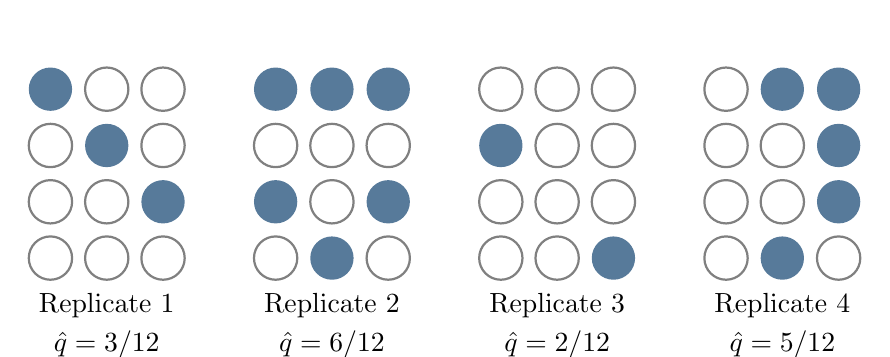
\begin{tikzpicture}[scale=0.55]
\foreach \rep/\pattern/\k [count=\c from 0] in {
  1/{1,0,0,0,1,0,0,0,1,0,0,0}/3,
  2/{1,1,1,0,0,0,1,0,1,0,1,0}/6,
  3/{0,0,0,1,0,0,0,0,0,0,0,1}/2,
  4/{0,1,1,0,0,1,0,0,1,0,1,0}/5}{
  \begin{scope}[xshift=\c*5.2cm]
  \foreach \v [count=\i from 0] in \pattern {
     \pgfmathtruncatemacro{\col}{mod(\i,3)}
     \pgfmathtruncatemacro{\row}{\i/3}
     \ifnum\v=1 \fill[accent!75] (\col*1.3,-\row*1.3) circle (0.5);
     \else \draw[thick, gray] (\col*1.3,-\row*1.3) circle (0.5); \fi
  }
  \node at (1.3,-5.0) {Replicate \rep};
  \node at (1.3,-5.9) {$\hat q=\k/12$};
  \end{scope}}
\end{tikzpicture}
\caption{Four replicates of a survey of $N=12$ people (filled = YES). The true $q$ never changes, but $\hat q$ changes from replicate to
replicate. The distribution of $\hat q$ over (infinitely many) replicates is its \textbf{sample distribution}; its spread is $\se(\hat q)$.}
\end{figure}

\begin{keybox}[title={Sample distribution and standard error}]
The \textbf{sample distribution} of $\hat\theta$ is its distribution over replicates of the data. The \textbf{standard error}
$\se(\hat\theta)$ is the standard deviation of the sample distribution. It answers: ``if I redid the whole study, by how much would my
estimate typically change?''
\end{keybox}

\begin{examplebox}[title={Example: the sample distribution of a Normal mean}]
Let $Y_1,\dots,Y_N\sim\Norm(\mu,\sigma^2)$ iid and estimate $\mu$ with $\hat\mu=\Ybar=\frac1N\sum_iY_i$.

$\sum_iY_i$ is a sum of independent Normals, so it is exactly Normal with mean $N\mu$ and variance $N\sigma^2$. Dividing by $N$ (which
divides the mean by $N$ and the variance by $N^2$):
\[
\hat\mu\sim\Norm\!\left(\mu,\ \frac{\sigma^2}{N}\right),\qquad \se(\hat\mu)=\frac{\sigma}{\sqrt N}.
\]
For non-Normal data with finite variance, the CLT gives the same statement as a large-$N$ approximation.
\end{examplebox}

\textbf{True vs.\ estimated standard error.} The formula $\sigma/\sqrt N$ contains $\sigma$, which in real life we do not know. So we
plug in an estimate, $\se(\hat\mu)=\hat\sigma/\sqrt N$. If we are working with a model whose parameters are given, ``standard error''
means the first formula; with real data it means the second. Some people call the distribution with $\hat\sigma$ plugged in the sample
distribution too.

\begin{examplebox}[title={Example: estimating $q$ (10/2 slides)}]
Let $Y_1,\dots,Y_N\sim\Bern(q)$ and $\hat q=\Ybar$. Now $\hat q$ is \emph{not} Normal (it can only take the values $0,\frac1N,\dots,1$),
but by the CLT the Normal result carries over for large $N$, with $\sigma^2=q(1-q)$:
\[
\hat q\approx\Norm\!\left(q,\ \frac{q(1-q)}{N}\right),\qquad \se(\hat q)=\sqrt{\frac{q(1-q)}{N}}.
\]
\end{examplebox}

\begin{figure}[h]
\centering
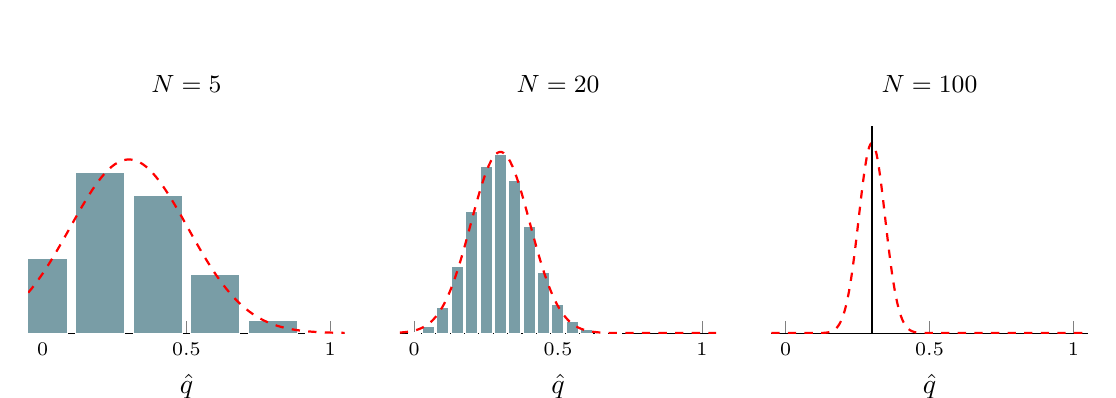
\begin{tikzpicture}
\begin{groupplot}[group style={group size=3 by 1, horizontal sep=0.7cm},
  width=5.6cm, height=4.3cm, xmin=-0.05, xmax=1.05, ymin=0, xlabel={$\hat q$}, yticklabels={}, ytick=\empty,
  tick label style={font=\scriptsize}, title style={font=\small}, axis x line*=bottom, axis y line=none]
\nextgroupplot[title={$N=5$}, ymax=2.4]
\addplot[ybar, bar width=0.17, fill=dataclr!60, draw=white] coordinates {(0.000,0.8404) (0.200,1.8007) (0.400,1.5435) (0.600,0.6615) (0.800,0.1417) (1.000,0.0121)};
\addplot[red, thick, dashed, domain=-0.05:1.05, samples=100] {exp(-(x-0.3)^2/(2*0.042))/sqrt(2*pi*0.042)};
\nextgroupplot[title={$N=20$}, ymax=4.6]
\addplot[ybar, bar width=0.042, fill=dataclr!60, draw=white] coordinates {(0.000,0.0160) (0.050,0.1368) (0.100,0.5569) (0.150,1.4321) (0.200,2.6084) (0.250,3.5773) (0.300,3.8328) (0.350,3.2852) (0.400,2.2879) (0.450,1.3074) (0.500,0.6163) (0.550,0.2401) (0.600,0.0772) (0.650,0.0204) (0.700,0.0044)};
\addplot[red, thick, dashed, domain=-0.05:1.05, samples=150] {exp(-(x-0.3)^2/(2*0.0105))/sqrt(2*pi*0.0105)};
\nextgroupplot[title={$N=100$}, ymax=9.8]
\addplot[red, thick, dashed, domain=-0.05:1.05, samples=250] {exp(-(x-0.3)^2/(2*0.0021))/sqrt(2*pi*0.0021)};
\addplot[black, thin] coordinates {(0.3,0) (0.3,9.5)};
\end{groupplot}
\end{tikzpicture}
\caption{Sample distribution of $\hat q=\Ybar$ for $q=0.3$. Bars: the exact distribution (scaled to a density). Red dashed: the CLT
approximation $\Norm(q,q(1-q)/N)$. As $N$ grows, the bars look more and more Normal and the distribution concentrates around $q=0.3$.}
\end{figure}

%==========================================================
\section{Bias, consistency, and the bias--variance trade-off (Unit 3.2)}
%==========================================================
\subsection{Definitions}
\begin{keybox}[title={MSE, bias, unbiased, consistent}]
\begin{itemize}[leftmargin=*,itemsep=2pt]
\item \textbf{Mean squared error:} $\MSE_{\hat\theta}=\E\big[(\hat\theta-\theta)^2\big]$, the average squared miss over replicates.
\item \textbf{Bias:} $\Bias=\E[\hat\theta]-\theta$. $\hat\theta$ is \textbf{unbiased} if the bias is $0$ for every $N$ (it is right on average).
\item \textbf{Consistent:} $\E[\hat\theta]\to\theta$ \emph{and} $\se(\hat\theta)\to0$ as $N\to\infty$ (more data pins down $\theta$).
\end{itemize}
\end{keybox}

\begin{keybox}[title={Bias--variance decomposition}]
\[
\MSE_{\hat\theta}=\se(\hat\theta)^2+\big(\E[\hat\theta]-\theta\big)^2=\text{variance}+\text{bias}^2.
\]
\inwords{the average squared error of an estimate is how much it jitters from dataset to dataset (variance) plus how far off it is on average (bias), squared.}
\end{keybox}
\textbf{Proof.} Apply the variance formula $\Var(W)=\E[W^2]-(\E W)^2$ to $W=\hat\theta-\theta$:
\begin{align*}
\Var(\hat\theta-\theta)&=\E\big[(\hat\theta-\theta)^2\big]-\big(\E[\hat\theta-\theta]\big)^2 \why{variance formula}\\
\Var(\hat\theta)&=\MSE_{\hat\theta}-\big(\E[\hat\theta]-\theta\big)^2. \why{$\theta$ is a constant: shifting does not change variance}
\end{align*}
Rearranging gives the result. $\square$

So an estimator can be wrong in two ways: it can be \emph{noisy} (large variance) or \emph{systematically off} (bias). The picture to
keep in mind is a dartboard: bias is how far the center of your throws is from the bullseye; variance is how spread out they are.

\begin{tipbox}[title={Unbiased and consistent are different}]
$\hat\mu_1=\Ybar+1/N$ is biased (bias $=1/N$) but consistent. $\hat\mu_2=(Y_1+Y_2)/2$ is unbiased
($\E\hat\mu_2=\mu$) but \emph{not} consistent: $\hat\mu_2\sim\Norm(\mu,\sigma^2/2)$, and its standard error $\sigma/\sqrt2$ never shrinks,
because it only ever uses two data points.
\end{tipbox}

\begin{examplebox}[title={Question (10/5): is the sample mean unbiased? consistent?}]
$\E[\Ybar]=q$ (Bernoulli) or $\mu$ (Normal), by the toolkit box, so it is unbiased.
$\se(\Ybar)=\sqrt{q(1-q)/N}$ or $\sigma/\sqrt N$, both $\to0$ as $N\to\infty$, so it is consistent.
\end{examplebox}

\subsection{Laplace's rule of succession}
The natural estimator of $q$ is $\hat q=\Ybar$. But if every $Y_i=0$ then $\hat q=0$: flip a coin twice, get two tails, and conclude the
coin can \emph{never} land heads. To fix this, pretend we have already seen two extra flips, one heads and one tails:
\[
\hat q_L=\frac{S+1}{N+2},\qquad S=\sum_iY_i\sim\Bin(N,q).
\]
\begin{examplebox}[title={Question (10/5): find the bias, variance and MSE of $\hat q_L$}]
\textbf{Mean.} Using $\E[S]=Nq$ and linearity,
\[
\E[\hat q_L]=\frac{\E[S]+1}{N+2}=\frac{Nq+1}{N+2}.
\]
\textbf{Bias.} Put both terms over the common denominator $N+2$:
\[
\Bias=\frac{Nq+1}{N+2}-q=\frac{Nq+1-q(N+2)}{N+2}=\frac{Nq+1-Nq-2q}{N+2}=\frac{1-2q}{N+2}.
\]
\textbf{Variance.} $\hat q_L=\frac{1}{N+2}S+\frac{1}{N+2}$ is $aS+b$ with $a=\frac1{N+2}$, so
\[
\Var(\hat q_L)=\frac{\Var(S)}{(N+2)^2}=\frac{Nq(1-q)}{(N+2)^2}.
\]
\textbf{MSE} $=$ variance $+$ bias$^2$:
\[
\MSE_{\hat q_L}=\frac{Nq(1-q)+(1-2q)^2}{(N+2)^2}.
\]
\textbf{Verdict.} Biased (unless $q=\tfrac12$, where $1-2q=0$), but consistent: the bias has $N$ in the denominator, and the variance
behaves like $N/N^2=1/N$; both go to $0$.

\textbf{Is the bias worth it?} Compare with $\Ybar$, whose MSE is just its variance $q(1-q)/N$. At $N=2$, $q=\tfrac12$:
$\MSE_{\Ybar}=0.25/2=0.125$ but $\MSE_{\hat q_L}=2(0.25)/16=0.031$. Laplace's estimator is four times more accurate there, even though it
is biased. At $q=0$ it loses ($\Ybar$ is then always exactly right). Unbiased is not automatically best.
\end{examplebox}

\begin{figure}[h]
\centering
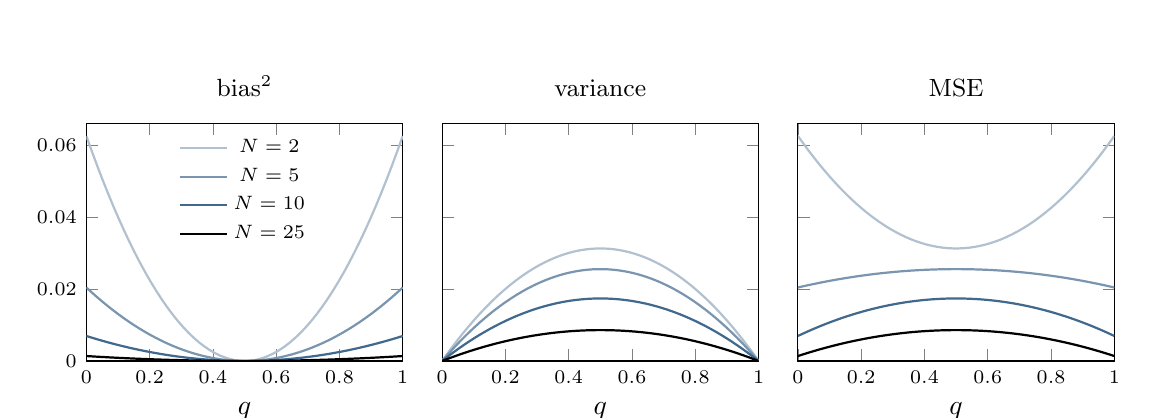
\begin{tikzpicture}
\begin{groupplot}[group style={group size=3 by 1, horizontal sep=0.5cm, y descriptions at=edge left},
  width=5.6cm, height=4.6cm, xmin=0, xmax=1, ymin=0, ymax=0.066, xlabel={$q$},
  tick label style={font=\scriptsize}, title style={font=\small}, scaled y ticks=false,
  yticklabel style={/pgf/number format/fixed, /pgf/number format/precision=2},
  cycle list={{accent!35,thick},{accent!60,thick},{accent!85,thick},{black,thick}}]
\nextgroupplot[title={bias$^2$}, legend style={font=\scriptsize, at={(0.5,0.98)}, anchor=north, draw=none, fill=none}]
\foreach \N in {2,5,10,25}{ \addplot+[no marks, domain=0:1, samples=60] {((1-2*x)/(\N+2))^2}; }
\legend{$N=2$,$N=5$,$N=10$,$N=25$}
\nextgroupplot[title={variance}]
\foreach \N in {2,5,10,25}{ \addplot+[no marks, domain=0:1, samples=60] {\N*x*(1-x)/(\N+2)^2}; }
\nextgroupplot[title={MSE}]
\foreach \N in {2,5,10,25}{ \addplot+[no marks, domain=0:1, samples=60] {(\N*x*(1-x)+(1-2*x)^2)/(\N+2)^2}; }
\end{groupplot}
\end{tikzpicture}
\caption{Bias$^2$, variance and MSE of Laplace's estimator, from the formulas above. Bias is largest near $q=0$ and $q=1$ (the estimator
is pulled toward $\tfrac12$); variance is largest at $q=\tfrac12$. All three shrink as $N$ grows.}
\end{figure}

The slides check these formulas by simulation. Each pass through the inner loop is one replicate of the data, so \py{q\_hat} holds $R$
draws from the sample distribution of $\hat q_L$. Then the sample bias$^2$, variance and MSE of those draws estimate the true ones:
\begin{lstlisting}
N = 10
R = 1000                      # number of replicates
qs = np.linspace(0, 1, 11)
for i in range(len(qs)):
    q = qs[i]
    q_hat = np.zeros(R)
    for r in range(R):
        S = np.random.binomial(N, q)
        # This also works:
        # ys = np.random.choice([0, 1], N, p=[1-q, q])
        # S = np.sum(ys)
        q_hat[r] = (S + 1) / (N + 2)
    bias2[i] = (np.mean(q_hat) - q)**2
    var[i] = np.var(q_hat)
    mse[i] = np.mean((q_hat - q)**2)
\end{lstlisting}

\subsection{Estimating the variance: Bessel's correction}
\begin{examplebox}[title={Question (10/5): $\mu$ known}]
If $Y_i\sim\Norm(\mu,\sigma^2)$ and we \emph{know} $\mu$, is $\hat\sigma_\mu^2=\frac1N\sum_i(Y_i-\mu)^2$ unbiased?

Yes: $\E[(Y_i-\mu)^2]=\Var(Y_i)=\sigma^2$ by the definition of variance, so
$\E[\hat\sigma_\mu^2]=\frac1N\sum_i\sigma^2=\frac1N\cdot N\sigma^2=\sigma^2$.
\end{examplebox}

Usually $\mu$ is unknown, so we use $\Ybar$ in its place: $\hat\sigma_0^2=\frac1N\sum_i(Y_i-\Ybar)^2$. This one is \textbf{biased}.
The trick to see why: add and subtract $\mu$ inside the square, then expand $(a-b)^2=a^2-2ab+b^2$ with $a=Y_i-\mu$ and $b=\Ybar-\mu$:
\begin{align*}
\sum_i(Y_i-\Ybar)^2&=\sum_i\big[(Y_i-\mu)-(\Ybar-\mu)\big]^2 \why{add and subtract $\mu$}\\
&=\sum_i(Y_i-\mu)^2-2(\Ybar-\mu)\sum_i(Y_i-\mu)+N(\Ybar-\mu)^2 \why{expand; $\Ybar-\mu$ same for all $i$}\\
&=\sum_i(Y_i-\mu)^2-2N(\Ybar-\mu)^2+N(\Ybar-\mu)^2 \why{$\sum_i(Y_i-\mu)=N(\Ybar-\mu)$}\\
&=\sum_i(Y_i-\mu)^2-N(\Ybar-\mu)^2.
\end{align*}
Now take expectations. $\E[(Y_i-\mu)^2]=\sigma^2$, and $\E[(\Ybar-\mu)^2]=\Var(\Ybar)=\sigma^2/N$ (because $\E\Ybar=\mu$). So
\[
\E\Big[\sum_i(Y_i-\Ybar)^2\Big]=N\sigma^2-N\cdot\frac{\sigma^2}{N}=(N-1)\sigma^2,
\qquad\text{so}\qquad \E[\hat\sigma_0^2]=\frac{N-1}{N}\sigma^2.
\]
\textbf{Why too small?} $\Ybar$ is computed from the same data, so it sits closer to the data points than the true $\mu$ does. Measuring
spread around $\Ybar$ therefore underestimates spread around $\mu$; the bias is $-\sigma^2/N$.

\begin{keybox}[title={Bessel's correction}]
Dividing by $N-1$ instead of $N$ removes the bias:
\[
\hat\sigma^2=\frac{1}{N-1}\sum_i(Y_i-\Ybar)^2,\qquad \E[\hat\sigma^2]=\sigma^2.
\]
$\hat\sigma_0^2$ is biased but still consistent (its bias $-\sigma^2/N\to0$). For large $N$ the two barely differ.
\inwords{when the mean is estimated from the same data, divide the sum of squared deviations by $N-1$ instead of $N$ to get the variance right on average.}
\end{keybox}

\begin{examplebox}[title={Check with $N=2$}]
With two points, $\Ybar=(Y_1+Y_2)/2$, so $Y_1-\Ybar=(Y_1-Y_2)/2$ and $Y_2-\Ybar=-(Y_1-Y_2)/2$. Then
$\hat\sigma_0^2=\frac12\big[\frac{(Y_1-Y_2)^2}{4}+\frac{(Y_1-Y_2)^2}{4}\big]=\frac{(Y_1-Y_2)^2}{4}$.
Since $\E[Y_1-Y_2]=0$, $\E[(Y_1-Y_2)^2]=\Var(Y_1-Y_2)=\sigma^2+\sigma^2=2\sigma^2$, so $\E[\hat\sigma_0^2]=\sigma^2/2$, which matches
$\frac{N-1}{N}\sigma^2$ at $N=2$.
\end{examplebox}

%==========================================================
\section{Confidence intervals (Unit 3.3)}
%==========================================================
\subsection{True vs.\ estimated sample distribution}
For $Y_i\sim\Norm(\mu,\sigma^2)$, the \emph{true} sample distribution of $\hat\mu=\Ybar$ is $\Norm(\mu,\sigma^2/N)$. But we know neither
$\mu$ nor $\sigma$! So we plug in our estimates to get the \textbf{estimated sample distribution}
\[
\hat\mu\approx\Norm\!\left({\color{red}\hat\mu},\ \frac{{\color{red}\hat\sigma}^2}{N}\right)\qquad\text{(red: numbers computed from our data).}
\]
This estimated distribution is itself random (it is centered at $\hat\mu$, not $\mu$, and its width uses $\hat\sigma$). Still, its width
tells us how far $\mu$ might plausibly be from $\hat\mu$. Confidence intervals make this precise.

\subsection{The 95\% confidence interval}
\begin{keybox}[title={95\% confidence interval}]
\[
\text{CI}=\Big[\hat\theta-1.96\,\se(\hat\theta),\ \ \hat\theta+1.96\,\se(\hat\theta)\Big].
\]
\inwords{go $1.96$ standard errors either side of the estimate; intervals built this way contain the true value in $95\%$ of repeated studies.}
\end{keybox}
\textbf{Why 1.96?} If the sample distribution is approximately Normal, $95\%$ of it lies within $1.96$ standard errors of its center. So
in $95\%$ of replicates $\hat\theta$ lands within $1.96\,\se$ of $\theta$, which is the same as saying $\theta$ lands within $1.96\,\se$ of
$\hat\theta$, i.e.\ inside the CI.

\begin{figure}[h]
\centering
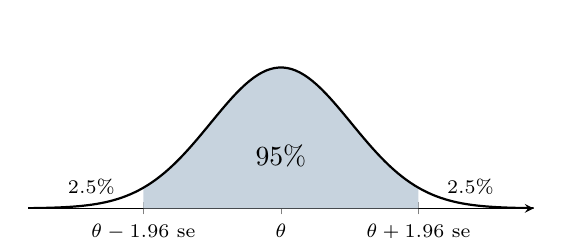
\begin{tikzpicture}
\begin{axis}[width=8cm, height=3.6cm, axis x line=bottom, axis y line=none, xmin=-3.6, xmax=3.6, ymin=0, ymax=0.45,
  xtick={-1.96,0,1.96}, xticklabels={$\theta-1.96\,\se$,$\theta$,$\theta+1.96\,\se$}, tick label style={font=\scriptsize}]
\addplot[fill=accent!25, draw=none, domain=-1.96:1.96, samples=80] {exp(-x^2/2)/sqrt(2*pi)} \closedcycle;
\addplot[thick, domain=-3.6:3.6, samples=120] {exp(-x^2/2)/sqrt(2*pi)};
\node at (axis cs:0,0.15) {$95\%$};
\node[font=\scriptsize] at (axis cs:-2.7,0.06) {$2.5\%$};
\node[font=\scriptsize] at (axis cs:2.7,0.06) {$2.5\%$};
\end{axis}
\end{tikzpicture}
\caption{An (approximately) Normal sample distribution. $95\%$ of replicates give $\hat\theta$ within $1.96$ standard errors of $\theta$.}
\end{figure}

\textbf{The $t$ multiplier.} With $\hat\sigma$ plugged in, $(\hat\mu-\mu)/\se(\hat\mu)$ is not exactly $\Norm(0,1)$; it has a
\textbf{$t$ distribution}, which looks Normal but has heavier tails (because $\hat\sigma$ is random too). The exact $95\%$ multiplier is
then a bit bigger than $1.96$: about $2.78$ for $N=5$, $2.26$ for $N=10$, $2.05$ for $N=30$, and $\approx1.96$ for large $N$. For
$N\gtrsim30$ the difference is negligible. Software such as statsmodels reports $t$-based numbers, so they may differ slightly from yours.

\begin{figure}[h]
\centering
\pgfmathsetseed{21}
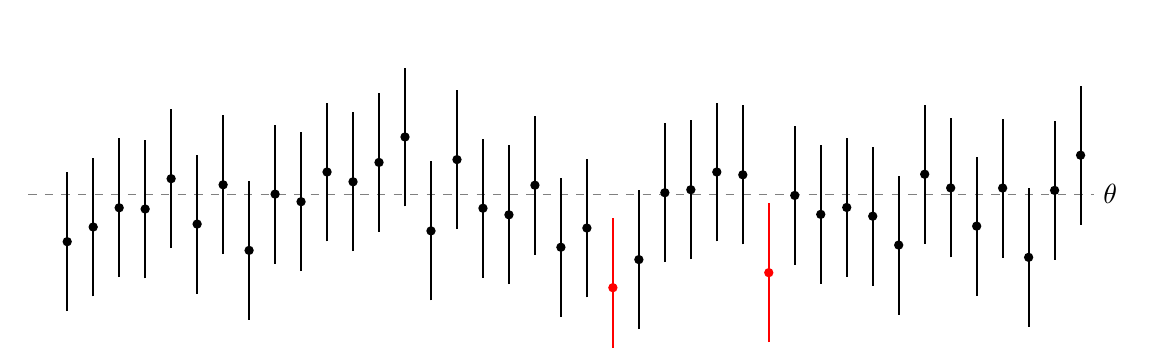
\begin{tikzpicture}[xscale=0.33, yscale=0.9]
\draw[dashed, gray] (-0.5,0) -- (40.5,0) node[right, black] {$\theta$};
\foreach \i in {1,...,40}{
  \pgfmathsetmacro{\c}{0.5*sqrt(-2*ln(0.001+0.998*rnd))*cos(360*rnd)}
  \pgfmathtruncatemacro{\miss}{abs(\c)>0.98 ? 1 : 0}
  \ifnum\miss=1 \def\clr{red}\else\def\clr{black}\fi
  \draw[\clr, thick] (\i,\c-0.98) -- (\i,\c+0.98);
  \fill[\clr] (\i,\c) circle (0.18 and 0.066);
}
\end{tikzpicture}
\caption{Each bar is the $95\%$ CI from one simulated replicate, with a dot at $\hat\theta$. The CIs move around; $\theta$ (dashed) does not.
About $95\%$ of the bars cover $\theta$; the red ones miss.}
\end{figure}

\subsection{Interpreting a CI correctly (optional subtlety)}
\begin{itemize}[leftmargin=*,itemsep=2pt]
\item \textbf{Correct:} if we generate many replicates of the data, the true $\theta$ falls in the resulting CI for $95\%$ of them; that is,
$\P(\theta\in\text{CI})=0.95$ where the CI is treated as a \emph{random} interval.
\item \textbf{Not correct:} ``there is a $95\%$ chance $\theta$ lies in \emph{this particular} interval.'' Once we compute, say,
$\text{CI}=[0.2,1.4]$, nothing is random any more: $\theta$ is either in it or not, so $\P(\theta\in\text{CI})$ is $0$ or $1$.
\end{itemize}
For practical purposes you can think of the CI as ``the region where the parameter is likely to be.''

\begin{examplebox}[title={Example (notes): how much data for a target CI width?}]
Model $Y_i\sim\Norm(\mu,\sigma^2)$, estimate $\mu$ by $\Ybar$, and from earlier experiments $\sigma\approx1$. How large must $N$ be for the
$95\%$ CI $\hat\mu\pm1.96\,\se(\hat\mu)$ to be no wider than $\hat\mu\pm0.25$?

The half-width is $1.96\,\se=1.96/\sqrt N$. We need
\[
\frac{1.96}{\sqrt N}\le0.25\ \Longrightarrow\ \sqrt N\ge\frac{1.96}{0.25}=7.84\ \Longrightarrow\ N\ge7.84^2\approx61.5,
\]
so $N=62$. (Since $\sigma\approx1$ is itself an estimate, this is approximate.) Notice the square: halving the width needs four times
the data.
\end{examplebox}

%==========================================================
\section{Hypothesis testing (Unit 3.6)}
%==========================================================
Often we estimate a parameter to make a \emph{decision}: is a drug worth pursuing? Do two graders grade differently? The procedure:
\begin{enumerate}[leftmargin=*,itemsep=2pt]
\item State a \textbf{null hypothesis} $H_0$ we might want to rule out, e.g.\ $H_0:\beta_1=0$ (``no effect'').
\item Compute a \textbf{test statistic} $\hat T$ from the data. For a regression slope we use how many standard errors the estimate is from $0$:
\[\hat T=\frac{\hat\beta_1}{\se(\hat\beta_1)}.\]
\item Ask: if $H_0$ were true, how likely is a test statistic at least as extreme as ours? Let $\hat T^*$ be the test statistic from a
replicate generated under $H_0$. Then $\hat T^*\approx\Norm(0,1)$, and the \textbf{$p$-value} is
\[ p_v=\P\big(|\hat T^*|>|\hat T|\big). \]
\end{enumerate}
A small $p_v$ means our data would be very surprising if $H_0$ were true, so we \emph{reject} $H_0$. A large $p_v$ means data like ours are
typical under $H_0$, so we \emph{cannot reject} it (which is not the same as proving $H_0$ true). Note the connection to CIs: $|\hat T|>1.96$
exactly when the $95\%$ CI does not contain $0$, and then $p_v<0.05$.

\begin{examplebox}[title={Example (notes): a clinical trial is a binary-predictor regression}]
Effect $Y$ in a control group ($X=0$) and a treatment group ($X=1$), $N/2$ people each, with $\sigma_\epsilon$ known:
$Y\given X\sim\Norm\big(\mu_C(1-X)+\mu_TX,\ \sigma_\epsilon^2\big)$. Since $\mu_C(1-X)+\mu_TX=\mu_C+(\mu_T-\mu_C)X$, this is a regression
with $\beta_0=\mu_C$ and $\beta_1=\mu_T-\mu_C$.

Each group mean is the average of $N/2$ Normals, so $\hat\mu_C\sim\Norm(\mu_C,\frac{\sigma_\epsilon^2}{N/2})$ and likewise for $\hat\mu_T$.
The two groups are independent, so variances add for the difference:
\[
\hat\beta_1=\hat\mu_T-\hat\mu_C\sim\Norm\!\left(\beta_1,\ \frac{2\sigma_\epsilon^2}{N}+\frac{2\sigma_\epsilon^2}{N}\right)=\Norm\!\left(\beta_1,\ \frac{4\sigma_\epsilon^2}{N}\right).
\]
Under $H_0:\beta_1=0$ the replicate $\hat\beta_1^*\sim\Norm(0,4\sigma_\epsilon^2/N)$, so $\hat T^*=\hat\beta_1^*/\se(\hat\beta_1)\sim\Norm(0,1)$.
\end{examplebox}

\begin{examplebox}[title={Worked example (10/7): do the two midterm graders grade differently?}]
Midterm 1 was graded by E ($X=1$, $N_E=23$ exams) and G ($X=0$, $N_G=45$). Model: $Y\given X\sim\Norm(\beta_0+\beta_1X,\sigma_\epsilon^2)$,
so $\beta_1$ is the difference in average score between graders.

\textbf{Sample distribution of $\hat\beta_1$ (``eyeball'' numbers from the plot).} $\overline{Y|X{=}0}\approx17$,
$\overline{Y|X{=}1}\approx17.5$, $\hat\sigma_\epsilon\approx5$. Each group mean is approximately Normal with variance $\hat\sigma_\epsilon^2/(\text{group size})$:
\[
\overline{Y|X{=}1}\approx\Norm(17.5,\ 25/23),\qquad \overline{Y|X{=}0}\approx\Norm(17,\ 25/45).
\]
The groups are independent, so for the difference the means subtract and the variances add. Using $25/23+25/45\approx1+\tfrac12$:
\[
\hat\beta_1=\overline{Y|X{=}1}-\overline{Y|X{=}0}\approx\Norm\big(\tfrac12,\ \tfrac32\big).
\]
\textbf{95\% CI.} $\se(\hat\beta_1)\approx\sqrt{3/2}\approx1.2$. Using $1.96\approx2$: $\text{CI}\approx[\tfrac12-2(1.2),\ \tfrac12+2(1.2)]\approx[-2,3]$,
which contains $0$.

\textbf{Test statistic.} $\hat T=\hat\beta_1/\se(\hat\beta_1)\approx0.5/1.2\approx0.4$: the difference is only $0.4$ standard errors from $0$.

\textbf{$p$-value by hand.} Near its center the standard Normal density is about $1/\sqrt{2\pi}\approx0.4$, so the area between $-0.4$
and $0.4$ is roughly a rectangle of width $0.8$ and height $0.4$: $\P(|\hat T^*|<0.4)\approx0.32$. Hence $p_v=\P(|\hat T^*|>0.4)\approx0.7$
(the exact value $2(1-\Phi(0.4))$ is $0.69$). A difference like ours is completely typical if the graders grade the same, so we
\emph{cannot reject} $H_0$.

\textbf{In Python} (with \py{x}, \py{y} numpy arrays) the exact numbers are:
\begin{lstlisting}
y0 = y[x == 0]
y1 = y[x == 1]
b1_hat = np.mean(y1) - np.mean(y0)
var_b1 = np.std(y1)**2/len(y1) + np.std(y0)**2/len(y0)
\end{lstlisting}
giving $\hat\beta_1\approx\Norm(0.68,\ 1.84)$, close to the eyeball answer.
\end{examplebox}

\begin{figure}[h]
\centering
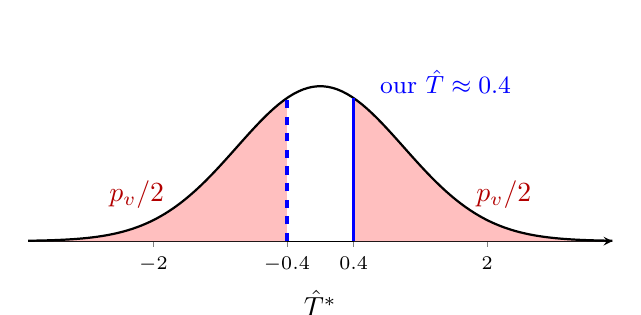
\begin{tikzpicture}
\begin{axis}[width=9cm, height=3.8cm, axis x line=bottom, axis y line=none, xmin=-3.5, xmax=3.5, ymin=0, ymax=0.45,
  xtick={-2,-0.4,0.4,2}, xlabel={$\hat T^*$}, tick label style={font=\scriptsize}]
\addplot[fill=red!25, draw=none, domain=-3.5:-0.4, samples=60] {exp(-x^2/2)/sqrt(2*pi)} \closedcycle;
\addplot[fill=red!25, draw=none, domain=0.4:3.5, samples=60] {exp(-x^2/2)/sqrt(2*pi)} \closedcycle;
\addplot[thick, domain=-3.5:3.5, samples=120] {exp(-x^2/2)/sqrt(2*pi)};
\addplot[blue, very thick] coordinates {(0.4,0) (0.4,0.368)};
\addplot[blue, very thick, dashed] coordinates {(-0.4,0) (-0.4,0.368)};
\node[red!70!black] at (axis cs:-2.2,0.12) {$p_v/2$};
\node[red!70!black] at (axis cs:2.2,0.12) {$p_v/2$};
\node[blue, font=\small, anchor=west] at (axis cs:0.6,0.41) {our $\hat T\approx0.4$};
\end{axis}
\end{tikzpicture}
\caption{The null distribution of $\hat T^*$. The $p$-value is the shaded area beyond $\pm|\hat T|$: here about $0.7$, so most of the curve.}
\end{figure}

\subsection{$p$-values are not $R^2$}
\begin{keybox}[title={The test statistic and $R^2$ (one predictor)}]
\[
\hat T^2=(N-2)\,\frac{R^2}{1-R^2}.
\]
\inwords{with one predictor, $\hat T$ depends only on $R^2$ and $N$: a high $R^2$ always gives a big $|\hat T|$ (tiny $p$-value), but a tiny $p$-value can come with a low $R^2$ when $N$ is large.}
\end{keybox}
\textbf{Derivation} (uses Section~\ref{sec:ls}; skip on a first read). Write $S_{xx}=\sum_i(X_i-\Xbar)^2$. The residual is
$r_i=(Y_i-\Ybar)-\hat\beta_1(X_i-\Xbar)$ (because $\hat\beta_0=\Ybar-\hat\beta_1\Xbar$). Squaring and summing,
\begin{align*}
\SSR&=\sum_i(Y_i-\Ybar)^2-2\hat\beta_1\sum_i(X_i-\Xbar)(Y_i-\Ybar)+\hat\beta_1^2S_{xx}\\
&=\SST-2\hat\beta_1(\hat\beta_1S_{xx})+\hat\beta_1^2S_{xx}=\SST-\hat\beta_1^2S_{xx}
\why{$\sum_i(X_i-\Xbar)(Y_i-\Ybar)=\hat\beta_1S_{xx}$}
\end{align*}
so $\hat\beta_1^2S_{xx}=\SST-\SSR$. With $\se(\hat\beta_1)^2=\hat\sigma_\epsilon^2/S_{xx}=\SSR/((N-2)S_{xx})$,
\[
\hat T^2=\frac{\hat\beta_1^2}{\se(\hat\beta_1)^2}=\frac{(N-2)\,\hat\beta_1^2S_{xx}}{\SSR}=\frac{(N-2)(\SST-\SSR)}{\SSR}
=(N-2)\frac{1-\SSR/\SST}{\SSR/\SST}=(N-2)\frac{R^2}{1-R^2}.
\]

\begin{examplebox}[title={Question (10/9): which scenarios are possible? ($p_v$ is for $H_0:\beta_1=0$, $N>3$)}]
\textbf{(a) $p_v=10^{-5}$ and $R^2=10^{-2}$: possible.} $R^2$ small means $X$ explains little of $Y$; but with a huge $N$ even a tiny
slope is measured precisely. From the formula, $\hat T^2\approx0.0101(N-2)$; $p_v=10^{-5}$ needs $|\hat T|\approx4.4$, i.e.\ $N\approx1950$.

\textbf{(b) $p_v=0.5$ and $R^2=0.99$: impossible.} $R^2=0.99$ forces $\hat T^2=99(N-2)\ge198$, so $|\hat T|\ge14$ and $p_v$ is tiny.

\textbf{(c) $\hat\beta_1=1000$, $\hat\sigma_\epsilon^2=10^{-5}$, $R^2=10^{-4}$: possible.} A big slope does not mean a big $R^2$:
$R^2\approx\beta_1^2\sigma_X^2/(\beta_1^2\sigma_X^2+\sigma_\epsilon^2)$, which is tiny if $X$ barely varies ($\sigma_X\approx3\times10^{-8}$).
\end{examplebox}

\textbf{Lessons from the ``guess $R^2$ and $p_v$'' plots (10/9).}
\begin{itemize}[leftmargin=*,itemsep=2pt]
\item A U-shaped pattern can have $R^2\approx0$ and a large $p_v$: there is a strong relationship, just not a \emph{linear} one.
\item A noisy cloud with a slight trend and many points can have small $R^2$ (0.10) but a tiny $p_v$ ($3\times10^{-6}$).
\item Real data with a clear trend (dog weight vs.\ life expectancy, $R^2=0.44$; bitcoin log price vs.\ year, $0.86$; CO$_2$, $0.98$) have
astronomically small $p_v$. A tiny $p_v$ says the slope is not $0$; it does not say the line is a good model (the CO$_2$ data curve).
\end{itemize}

%==========================================================
\section{Least squares for single-predictor regression (Unit 3.4)}\label{sec:ls}
%==========================================================
\subsection{The estimators}
Data $(X_1,Y_1),\dots,(X_N,Y_N)$ from $Y\given X\sim\Norm(\beta_0+\beta_1X,\sigma_\epsilon^2)$. How do we estimate $\beta_1$? We know
$\beta_1=\Cov(X,Y)/\sigma_X^2$, and both are expectations:
$\Cov(X,Y)=\E[(X-\E X)(Y-\E Y)]$, $\sigma_X^2=\E[(X-\E X)^2]$.
Replace each expectation by a sample average, $\E[\,\cdot\,]\to\frac1N\sum_i$, and $\E X,\E Y$ by $\Xbar,\Ybar$:
\[
\Cov(X,Y)\approx\frac1N\sum_i(X_i-\Xbar)(Y_i-\Ybar),\qquad \sigma_X^2\approx\frac1N\sum_i(X_i-\Xbar)^2.
\]
The $\frac1N$'s cancel in the ratio. For the intercept, $\E Y=\beta_0+\beta_1\E X$ gives $\beta_0=\E Y-\beta_1\E X$.
\begin{keybox}[title={Least squares estimators}]
\[
\hat\beta_1=\frac{\sum_i(X_i-\Xbar)(Y_i-\Ybar)}{\sum_i(X_i-\Xbar)^2},\qquad \hat\beta_0=\Ybar-\hat\beta_1\Xbar.
\]
\inwords{the slope is the sample covariance of $X$ and $Y$ divided by the sample variance of $X$; the intercept makes the line pass through the point of averages $(\Xbar,\Ybar)$.}
\end{keybox}
The fitted line always passes through the point $(\Xbar,\Ybar)$: plug $X=\Xbar$ into $\hat\beta_0+\hat\beta_1X$ to get $\Ybar$.

\subsection{Residuals, SSR, SST, $\hat\sigma_\epsilon^2$, $R^2$}
The \textbf{residuals} are the vertical distances from each point to the fitted line, $r_i=Y_i-(\hat\beta_0+\hat\beta_1X_i)$.
\[
\SSR=\sum_ir_i^2\ \ \text{(sum of squared residuals)},\qquad \SST=\sum_i(Y_i-\Ybar)^2\ \ \text{(total sum of squares)}.
\]
(Careful with other books: some use ``SSR'' for the \emph{regression} sum of squares $\SST-\mathrm{SSE}$, a different thing.)
\begin{keybox}[title={Estimators of the noise variance and of $\rho^2$}]
\[
\hat\sigma_\epsilon^2=\frac{\SSR}{N-2}\approx\frac{\SSR}{N},\qquad\qquad \hat\rho^2=R^2=1-\frac{\SSR}{\SST}.
\]
\inwords{$\hat\sigma_\epsilon^2$ is the average squared vertical distance from the points to the line (dividing by $N-2$); $R^2$ is the fraction of the total spread in $Y$ that the line accounts for.}
\end{keybox}
\textbf{Why these make sense.} $\SSR/N$ is the average squared scatter around the line, a sample version of $\sigma_\epsilon^2=\Var(Y\given X)$.
$\SST/N$ is the sample version of $\sigma_Y^2$. So $1-\SSR/\SST$ copies $\rho^2=1-\sigma_\epsilon^2/\sigma_Y^2$.
\textbf{Why $N-2$?} The same reason as Bessel's correction: two parameters ($\beta_0,\beta_1$) were fitted from the same data, which makes
the line sit a bit too close to the points; dividing by $N-2$ makes $\hat\sigma_\epsilon^2$ unbiased. It makes little difference once $N\gtrsim20$.

\subsection{Why ``least squares''}
\begin{keybox}[title={Least squares property}]
\[
(\hat\beta_0,\hat\beta_1)=\operatorname*{argmin}_{b_0,b_1}\ \sum_i\big(Y_i-b_0-b_1X_i\big)^2:
\]
of all lines, the least squares line has the smallest SSR. This holds for any set of points, wherever they came from.
\inwords{of every possible straight line, the least squares line makes the total of the squared vertical misses as small as possible.}
\end{keybox}

\textbf{Optional calculus check.} Call $f(b_0,b_1)=\sum_i(Y_i-b_0-b_1X_i)^2$. At the minimum, changing $b_0$ alone (holding $b_1$ fixed)
cannot lower $f$, so the ordinary derivative in $b_0$ is $0$; same for $b_1$. By the chain rule:
\begin{align*}
\text{in } b_0:\quad &\sum_i -2(Y_i-b_0-b_1X_i)=0\ \Longrightarrow\ N\Ybar-Nb_0-b_1N\Xbar=0\ \Longrightarrow\ b_0=\Ybar-b_1\Xbar,\\
\text{in } b_1:\quad &\sum_i -2X_i(Y_i-b_0-b_1X_i)=0.
\end{align*}
Substitute $b_0=\Ybar-b_1\Xbar$ into the second equation: $\sum_iX_i\big[(Y_i-\Ybar)-b_1(X_i-\Xbar)\big]=0$, so
$b_1=\dfrac{\sum_iX_i(Y_i-\Ybar)}{\sum_iX_i(X_i-\Xbar)}$. Finally, subtracting $\Xbar\sum_i(Y_i-\Ybar)=0$ from the top and
$\Xbar\sum_i(X_i-\Xbar)=0$ from the bottom (the toolkit trick) turns this into exactly the $\hat\beta_1$ formula.

\begin{figure}[h]
\centering
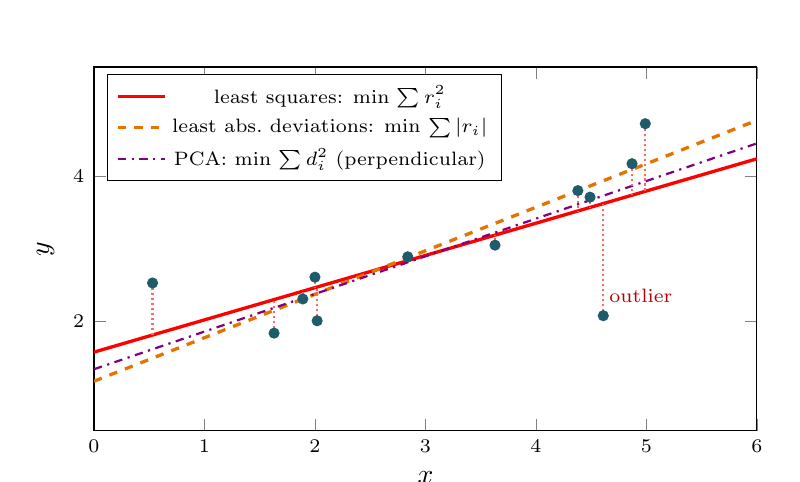
\begin{tikzpicture}
\begin{axis}[width=10cm, height=6.2cm, xmin=0, xmax=6, ymin=0.5, ymax=5.5, xlabel={$x$}, ylabel={$y$},
  legend style={font=\scriptsize, at={(0.02,0.98)}, anchor=north west}, tick label style={font=\scriptsize}]
\addplot[red, very thick, domain=0:6] {1.5794+0.4430*x};
\addplot[orange!90!black, very thick, dashed, domain=0:6] {1.1790+0.5979*x};
\addplot[violet, thick, dashdotted, domain=0:6] {1.3443+0.5175*x};
\foreach \xx/\yy in {0.53/2.53,1.63/1.84,1.89/2.31,2.00/2.61,2.02/2.01,2.84/2.89,3.63/3.05,4.38/3.80,4.49/3.71,4.61/2.08,4.87/4.17,4.99/4.72}{
  \edef\temp{\noexpand\draw[red!60, densely dotted, thick] (axis cs:\xx,\yy) -- (axis cs:\xx,{1.5794+0.4430*\xx});}\temp }
\addplot[only marks, mark=*, mark size=1.8pt, dataclr] coordinates {(0.53,2.53) (1.63,1.84) (1.89,2.31) (2.00,2.61) (2.02,2.01) (2.84,2.89) (3.63,3.05) (4.38,3.80) (4.49,3.71) (4.61,2.08) (4.87,4.17) (4.99,4.72)};
\legend{least squares: min $\sum r_i^2$, least abs.\ deviations: min $\sum|r_i|$, PCA: min $\sum d_i^2$ (perpendicular)}
\node[font=\scriptsize, red!70!black] at (axis cs:4.95,2.35) {outlier};
\end{axis}
\end{tikzpicture}
\caption{Made-up data with one outlier. Dotted red: the residuals $r_i$ of the least squares line. Three criteria give three different
lines. Because least squares \emph{squares} the residuals, the outlier's big residual counts heavily, and it pulls the LS line down
more than the least-absolute-deviations line. The perpendicular-distance (PCA) line treats $x$ and $y$ symmetrically. Minimizing SSR is the
right choice when the data come from a linear regression model.}
\end{figure}

\subsection{Two kinds of replicates}
$\hat\beta_0,\hat\beta_1$ are computed from random data, so they have sample distributions. For regression there are two ways to make a replicate:
\begin{itemize}[leftmargin=*,itemsep=2pt]
\item \textbf{Conditional on $X$:} keep the same $X_1,\dots,X_N$ and draw new $Y_i\given X_i$. Example: an experiment where we choose the doses.
\item \textbf{Not conditional on $X$:} draw new pairs $(X_i,Y_i)$. Example: a survey, where a new sample brings new people with new $X$'s.
\end{itemize}
We focus on the sample distribution \textbf{conditional on $X_1,\dots,X_N$}: the $X$'s are fixed numbers and only the $Y$'s are random.
Write $S_{xx}=\sum_i(X_i-\Xbar)^2\approx N\sigma_X^2$.

\subsection{$\hat\beta_1$ is unbiased}
Conditional on the $X$'s, the denominator $S_{xx}$ and each $(X_i-\Xbar)$ are constants, so linearity of $\E$ lets us move the expectation
onto the $Y$'s:
\begin{align*}
\E[\hat\beta_1\given X_1,\dots,X_N]&=\frac{\sum_i(X_i-\Xbar)\,\E[(Y_i-\Ybar)\given X_1,\dots,X_N]}{\sum_i(X_i-\Xbar)^2} \why{linearity}.
\end{align*}
From the model, $\E[Y_i\given X_i]=\beta_0+\beta_1X_i$, and averaging over $i$, $\E[\Ybar\given X_1,\dots,X_N]=\beta_0+\beta_1\Xbar$. So
\[
\E[(Y_i-\Ybar)\given X_1,\dots,X_N]=\beta_0+\beta_1X_i-\beta_0-\beta_1\Xbar=\beta_1(X_i-\Xbar),
\]
and therefore
\[
\E[\hat\beta_1\given X_1,\dots,X_N]=\frac{\sum_i(X_i-\Xbar)\,\beta_1(X_i-\Xbar)}{\sum_i(X_i-\Xbar)^2}=\beta_1\frac{\sum_i(X_i-\Xbar)^2}{\sum_i(X_i-\Xbar)^2}=\beta_1.
\]
Across replicates with the same $X$'s, $\hat\beta_1$ is right on average. (A similar argument shows $\E[\hat\beta_0\given X]=\beta_0$.)
The key ingredient: the noise $\epsilon_i$ is independent of \emph{all} the predictors. Section~\ref{sec:ar} shows what goes wrong without it.

\subsection{The sample distribution of $\hat\beta_1$}
\textbf{Variance (optional derivation; the notes state it without proof).} Because $\sum_i(X_i-\Xbar)\Ybar=\Ybar\cdot0=0$, we can drop
$\Ybar$ from the numerator: $\hat\beta_1=\frac{1}{S_{xx}}\sum_i(X_i-\Xbar)Y_i$. Given the $X$'s, this is a weighted sum of independent $Y_i$'s,
each with variance $\sigma_\epsilon^2$, so
\[
\Var(\hat\beta_1\given X)=\frac{1}{S_{xx}^2}\sum_i(X_i-\Xbar)^2\sigma_\epsilon^2=\frac{\sigma_\epsilon^2S_{xx}}{S_{xx}^2}=\frac{\sigma_\epsilon^2}{S_{xx}}.
\]
A weighted sum of Normals is Normal, and $S_{xx}\approx N\sigma_X^2$, so:
\begin{keybox}[title={Sample distribution of the slope}]
\[
\hat\beta_1\approx\Norm\!\left(\beta_1,\ \frac{\sigma_\epsilon^2}{N\sigma_X^2}\right),\qquad \se(\hat\beta_1)\approx\frac{\sigma_\epsilon}{\sigma_X\sqrt N}.
\]
The slope is pinned down better with \textbf{less noise} (small $\sigma_\epsilon$), \textbf{more spread-out $X$'s} (large $\sigma_X$), or
\textbf{more data} (large $N$). Intuition for $\sigma_X$: if all $X$'s are bunched together, a little noise can tilt the line a lot,
like balancing a ruler on two close fingers.
\inwords{across repeated datasets the estimated slope is centered on the true slope, and it varies less when the noise is small, the $X$'s are spread out, or there is more data.}
\end{keybox}

\begin{figure}[h]
\centering
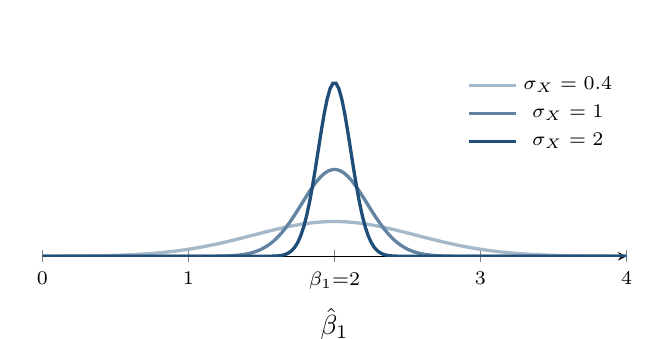
\begin{tikzpicture}
\begin{axis}[width=9cm, height=4cm, axis x line=bottom, axis y line=none, xmin=0, xmax=4, ymin=0, xlabel={$\hat\beta_1$},
  xtick={0,1,2,3,4}, xticklabels={0,1,$\beta_1{=}2$,3,4}, tick label style={font=\scriptsize},
  legend style={font=\scriptsize, draw=none, at={(1,1)}, anchor=north east}]
\addplot[accent!40, very thick, domain=0:4, samples=150] {exp(-(x-2)^2/(2*0.3125))/sqrt(2*pi*0.3125)};
\addplot[accent!70, very thick, domain=0:4, samples=150] {exp(-(x-2)^2/(2*0.05))/sqrt(2*pi*0.05)};
\addplot[accent, very thick, domain=0:4, samples=200] {exp(-(x-2)^2/(2*0.0125))/sqrt(2*pi*0.0125)};
\legend{$\sigma_X=0.4$,$\sigma_X=1$,$\sigma_X=2$}
\end{axis}
\end{tikzpicture}
\caption{$\Norm(\beta_1,\sigma_\epsilon^2/(N\sigma_X^2))$ with $N=20$, $\beta_1=2$, $\sigma_\epsilon=1$ (the 10/7 slide setting). Spreading the
$X$'s out by a factor of $5$ shrinks $\se(\hat\beta_1)$ by a factor of $5$.}
\end{figure}

\begin{examplebox}[title={Back to the graders (10/7)}]
$N=68$ exams, $N_E=23$ graded by E, $\hat\sigma_\epsilon\approx5$. Here $X\sim\Bern(p)$ with $p\approx23/68\approx1/3$, so
$\sigma_X^2=p(1-p)\approx\tfrac13\cdot\tfrac23=\tfrac29$ and $N\sigma_X^2\approx68\cdot\tfrac29=\tfrac{136}{9}\approx15.1$. Then
\[
\Var(\hat\beta_1)\approx\frac{\hat\sigma_\epsilon^2}{N\sigma_X^2}\approx\frac{25}{136/9}=\frac{225}{136}\approx1.65,\qquad \se(\hat\beta_1)\approx\sqrt{1.65}\approx1.29.
\]
Compare: back of the envelope, $\Var\approx3/2$ ($\se\approx1.2$); exact Python, $\Var=1.84$ ($\se\approx1.36$). All three roughly agree: the
boxed formula gives the same answer as the difference of means.
\end{examplebox}

\subsection{Computing everything in Python}
Using the covariance matrix:
\begin{lstlisting}
C = np.cov(x, y)
beta1_hat = C[0, 1] / C[0, 0]          # cov(x, y) / var(x)
\end{lstlisting}
\py{C} is the $2\times2$ \textbf{sample covariance matrix}
$\begin{pmatrix}\widehat{\Var}(X)&\widehat{\Cov}(X,Y)\\\widehat{\Cov}(X,Y)&\widehat{\Var}(Y)\end{pmatrix}$ with
$\widehat{\Cov}(X,Y)=\frac{1}{N-1}\sum_i(X_i-\Xbar)(Y_i-\Ybar)$. Python counts rows and columns from $0$, so \py{C[0, 1] / C[0, 0]}
is $\widehat{\Cov}/\widehat{\Var}(X)=\hat\beta_1$ (the $\frac1{N-1}$'s cancel). Directly from the formulas:
\begin{lstlisting}
beta1_hat = np.sum((x - np.mean(x)) * (y - np.mean(y))) \
            / np.sum((x - np.mean(x))**2)
beta0_hat = np.mean(y) - beta1_hat * np.mean(x)
r = y - (beta0_hat + beta1_hat * x)                 # residuals
sigma2_hat = np.sum(r**2) / (len(y) - 2)
R2 = 1 - np.sum(r**2) / np.sum((y - np.mean(y))**2)
se_beta1 = np.sqrt(sigma2_hat / np.sum((x - np.mean(x))**2))
T = beta1_hat / se_beta1
p_v = 2 * (1 - norm.cdf(np.abs(T)))                 # norm from scipy.stats
\end{lstlisting}
The last line is the $p$-value: $\P(|\hat T^*|>|\hat T|)$ is two tails, each $1-\Phi(|\hat T|)$.

\begin{examplebox}[title={Example (notes): TV advertising and sales}]
The Advertising data has $N=200$ markets, $X=$ TV budget (\$1000s), $Y=$ sales (1000s of units). Running the code above gives
$\hat\beta_0\approx7.03$, $\hat\beta_1\approx0.048$, $\SSR\approx2103$, $\SST\approx5417$, $\hat\sigma_\epsilon\approx3.26$, $R^2\approx0.61$.

Interpretation: each extra \$1000 of TV advertising goes with about $48$ more units sold ($0.048$ thousand), and the TV budget explains
about $61\%$ of the variation in sales between markets. Check: $1-2103/5417=0.61$ and $\sqrt{2103/198}=3.26$.

Model check by simulation: making ``fake'' datasets $\hat\beta_0+\hat\beta_1x+\Norm(0,\hat\sigma_\epsilon^2)$ shows constant spread, while the
real data fan out (residual SD about $1.8$ for budgets under 100, about $4.4$ over 200). So the constant-variance assumption is questionable here.
\end{examplebox}

%==========================================================
\section{Autoregressive models and the Hurwicz bias (Unit 3.5)}\label{sec:ar}
%==========================================================
\subsection{Time series and the AR(1) model}
A \textbf{time series} $Y_1,Y_2,\dots,Y_N$ is a sequence of measurements of the same thing at successive times; the running example is
$Y_t=\log(\text{bitcoin price on day }t)$. Goal: predict tomorrow's price, and the next day's\ldots

Using time as the predictor does not really make sense: prices on different days are not produced independently, so the points
$(t,Y_t)$ and $(t+1,Y_{t+1})$ are not independent. Instead we capture the fact that today's price depends on yesterday's.

\begin{keybox}[title={AR(1) model}]
An \textbf{autoregressive model} AR(1) is a regression whose predictor is the previous value of the response:
\[
Y_t\given Y_{t-1}\sim\Norm(\beta_0+\beta_1Y_{t-1},\ \sigma_\epsilon^2),\qquad\text{i.e.}\qquad Y_t=\beta_0+\beta_1Y_{t-1}+\epsilon_t,
\]
where $\epsilon_t$ is independent of everything \emph{before} time $t$ (but not of the future). The regression data are the pairs
\[
(X_1,Y_1),\dots,(X_{N-1},Y_{N-1})\ \longleftrightarrow\ (Y_1,Y_2),\ (Y_2,Y_3),\dots,(Y_{N-1},Y_N).
\]
\inwords{today's value is a straight-line function of yesterday's value plus fresh noise.}
\end{keybox}
Once you know $Y_{t-1}$, the earlier values $Y_{t-2},Y_{t-3},\dots$ tell you nothing more about $Y_t$. For bitcoin, least squares gives
$\hat\beta_1\approx0.9996$ and $\hat\sigma_\epsilon\approx0.016$ (with $\log_{10}$): today's log price is essentially yesterday's plus noise.

\subsection{Stationary AR(1) processes}
A series is \textbf{stationary} if its distribution does not change over time; in particular $Y_t$ and $Y_{t-1}$ have the same mean $\mu$
and the same standard deviation $\sigma_Y$. Three facts follow.

\textbf{1. The slope is a correlation.} The slope of any regression is $\Cov(X,Y)/\sigma_X^2$. Here $X=Y_{t-1}$ and $Y=Y_t$ have the same SD, so
\[
\beta_1=\frac{\Cov(Y_{t-1},Y_t)}{\sigma_Y^2}=\frac{\Cov(Y_{t-1},Y_t)}{\sigma_Y\,\sigma_Y}=\rho,
\]
the correlation between consecutive values. From now on we write $\rho$ for $\beta_1$.

\textbf{2. The mean.} Take expectations of $Y_t=\beta_0+\rho Y_{t-1}+\epsilon_t$, using $\E Y_t=\E Y_{t-1}=\mu$ and $\E\epsilon_t=0$:
\[
\mu=\beta_0+\rho\mu\ \Longrightarrow\ \beta_0=(1-\rho)\mu,\qquad\text{so}\qquad Y_t=\mu(1-\rho)+\rho Y_{t-1}+\epsilon_t,
\]
which can be rewritten as $Y_t-\mu=\rho(Y_{t-1}-\mu)+\epsilon_t$. When $|\rho|<1$, each step shrinks the deviation from the mean by a factor $\rho$
on average and then adds new noise: \textbf{regression to the mean}. Daughters of unusually tall mothers are tall, but on average less tall
than their mothers.

\textbf{3. The variance.} Take variances; $\epsilon_t$ is independent of $Y_{t-1}$, so the variances add:
\[
\sigma_Y^2=\rho^2\sigma_Y^2+\sigma_\epsilon^2\ \Longrightarrow\ \sigma_Y^2(1-\rho^2)=\sigma_\epsilon^2\ \Longrightarrow\ \sigma_Y^2=\frac{\sigma_\epsilon^2}{1-\rho^2}.
\]
The closer $\rho$ is to $1$, the more slowly the series returns to its mean, and the farther it wanders. Compare with Section 2:
$1-\rho^2=\sigma_\epsilon^2/\sigma_Y^2$ is the same identity.

\subsection{When $\rho\approx1$: the random walk}
If $\rho=1$, the formula gives $\sigma_Y^2=\infty$. How can that be? Take $\beta_0=0$, $Y_0=0$ and unroll the model:
\[
Y_{t+1}=Y_t+\epsilon_{t+1}=Y_{t-1}+\epsilon_t+\epsilon_{t+1}=\cdots=\sum_{s=1}^{t+1}\epsilon_s .
\]
$Y_t$ is a sum of $t$ independent $\Norm(0,\sigma_\epsilon^2)$ steps, so
\[
Y_t\sim\Norm(0,\ \sigma_\epsilon^2\,t).
\]
This is a \textbf{random walk}: the noise is never forgotten, and the variance grows forever instead of settling down. There is no stationary
distribution. With $\hat\beta_1\approx0.9996$, the bitcoin log price is very close to a random walk.

\begin{figure}[h]
\centering
\pgfmathsetseed{8}
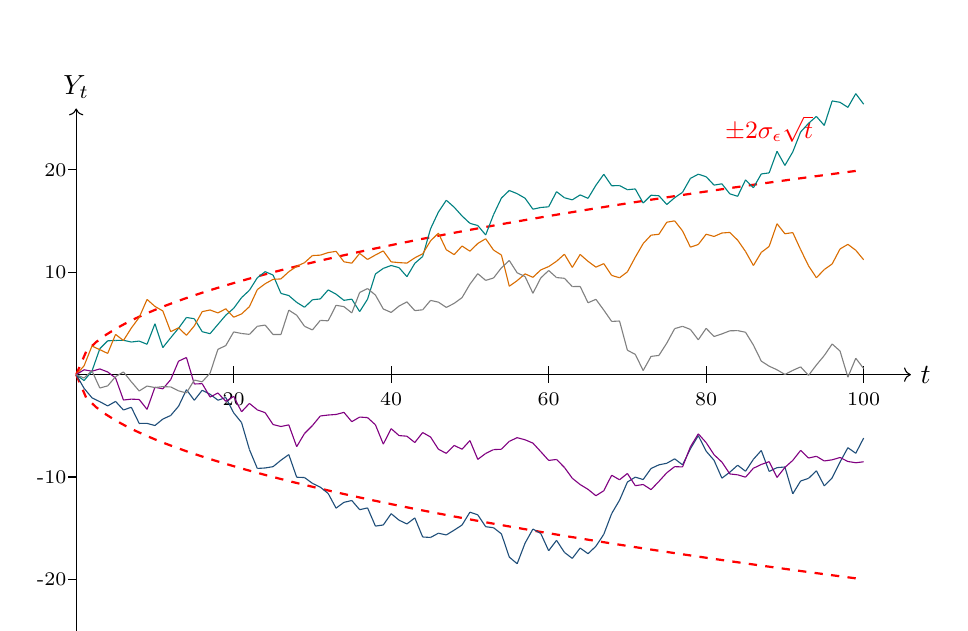
\begin{tikzpicture}[xscale=0.1, yscale=0.13]
\draw[->] (0,0) -- (106,0) node[right] {$t$};
\draw[->] (0,-26) -- (0,26) node[above] {$Y_t$};
\foreach \yy in {-20,-10,10,20} {\draw (-1,\yy) -- (0,\yy) node[left, font=\scriptsize] {\yy};}
\foreach \tt in {20,40,60,80,100} {\draw (\tt,-0.8) -- (\tt,0.8); \node[below, font=\scriptsize] at (\tt,-0.8) {\tt};}
\draw[red, dashed, thick, domain=0:100, samples=80] plot (\x,{2*sqrt(\x)});
\draw[red, dashed, thick, domain=0:100, samples=80] plot (\x,{-2*sqrt(\x)});
\node[red, font=\small] at (88,24) {$\pm2\sigma_\epsilon\sqrt t$};
\foreach \col in {accent,teal,orange!85!black,violet,gray}{
  \xdef\yold{0}
  \foreach \t in {1,...,100}{
    \pgfmathsetmacro{\ynew}{\yold+sqrt(-2*ln(0.001+0.998*rnd))*cos(360*rnd)}
    \draw[\col, thin] ({\t-1},\yold) -- (\t,\ynew);
    \xdef\yold{\ynew}
  }
}
\end{tikzpicture}
\caption{Five simulated random walks with $\sigma_\epsilon=1$. The envelope $\pm2\sigma_\epsilon\sqrt t$ (about $95\%$ of walks at each $t$) keeps widening.}
\end{figure}

\subsection{Why least squares is biased here: the Hurwicz bias}
Take $\mu=0$ for simplicity and fit $Y_t=\rho Y_{t-1}+\epsilon_t$ by least squares with no intercept (then $\hat\rho=\sum Y_{t-1}Y_t/\sum Y_{t-1}^2$).
Substitute the model into the numerator:
\begin{align*}
\E[\hat\rho]=\E\left[\frac{\sum_tY_{t-1}Y_t}{\sum_tY_{t-1}^2}\right]
&=\E\left[\frac{\sum_tY_{t-1}(\rho Y_{t-1}+\epsilon_t)}{\sum_tY_{t-1}^2}\right] \why{$Y_t=\rho Y_{t-1}+\epsilon_t$}\\
&=\rho+\E\left[\frac{\sum_tY_{t-1}\epsilon_t}{\sum_tY_{t-1}^2}\right]
\ \underset{\text{Hurwicz (1950)}}{\approx}\ \rho-\frac{2\rho}{N}. \why{split the fraction}
\end{align*}
\textbf{Why the second term is not zero.} In ordinary regression the noise $\epsilon_i$ is independent of \emph{all} of the predictors, so
conditional on the $X$'s the second term has mean $0$ and $\hat\beta_1$ is unbiased (that was the proof in Section~\ref{sec:ls}). In a time
series the predictors are $Y_1,\dots,Y_{N-1}$ themselves. Although $\epsilon_t$ is independent of the \emph{past} value $Y_{t-1}$, it is
part of $Y_t$, $Y_{t+1}$, and every later value, all of which appear in the denominator. The noise is correlated with the predictors that
come after it, so the argument breaks down.

\begin{keybox}[title={Hurwicz bias}]
For a finite series, least squares underestimates how persistent an AR(1) process is: $\E[\hat\rho]-\rho\approx-2\rho/N$. The estimator is
biased (pulled toward $0$) but consistent (the bias vanishes as $N\to\infty$). You do not need to memorize the formula; know \emph{why}
the bias exists.
\inwords{with a short series, the fitted $\hat\rho$ comes out too small on average, by about $2\rho/N$.}
\end{keybox}

\begin{examplebox}[title={Example (notes): seeing the bias by simulation}]
\begin{lstlisting}
rng = np.random.default_rng(42)
beta1 = 0.6

def fit_beta1_hat(N):
    eps = rng.normal(size=N)
    Y = np.empty(N)
    Y[0] = eps[0]
    for t in range(1, N):
        Y[t] = beta1 * Y[t - 1] + eps[t]
    y_lag, y = Y[:-1], Y[1:]
    return np.sum(y_lag * y) / np.sum(y_lag**2)

for N in [10, 50, 200]:
    beta1_hats = [fit_beta1_hat(N) for _ in range(20_000)]
    print(f"N={N}: average beta1_hat = {np.mean(beta1_hats):.3f}")
\end{lstlisting}
prints averages $0.506$, $0.577$, $0.595$ for $N=10,50,200$. Every one falls short of the true $0.6$, and the gap shrinks with $N$.
The formula predicts biases $-2(0.6)/50=-0.024$ and $-2(0.6)/200=-0.006$, matching the simulation; at $N=10$ the match is worse, because
the formula is only a large-$N$ approximation.
\end{examplebox}

\subsection{How fast do correlations decay? Autocorrelation}
The \textbf{autocorrelation at lag $k$} is $\rho_k=\corr(Y_t,Y_{t+k})$. For a stationary AR(1) with mean $0$, $Y_{t+1}=\rho Y_t+\epsilon_{t+1}$,
apply the model repeatedly:
\begin{align*}
Y_{t+1}&=\rho Y_t+\epsilon_{t+1}\\
Y_{t+2}&=\rho Y_{t+1}+\epsilon_{t+2}=\rho(\rho Y_t+\epsilon_{t+1})+\epsilon_{t+2}=\rho^2Y_t+\rho\,\epsilon_{t+1}+\epsilon_{t+2}\\
&\ \,\vdots\\
Y_{t+k}&=\rho^kY_t+\underbrace{\rho^{k-1}\epsilon_{t+1}+\cdots+\rho\,\epsilon_{t+k-1}+\epsilon_{t+k}}_{\text{future noise, independent of }Y_t}.
\end{align*}
By bilinearity, $\Cov(Y_t,Y_{t+k})=\rho^k\Cov(Y_t,Y_t)+0=\rho^k\sigma_Y^2$, and since $\Var(Y_{t+k})=\Var(Y_t)=\sigma_Y^2$:
\begin{keybox}[title={Autocorrelation of an AR(1)}]
\[
\rho_k=\frac{\Cov(Y_t,Y_{t+k})}{\sigma_Y\sigma_Y}=\rho^k .
\]
The correlation decays \emph{exponentially} in the lag. After $k=10$ steps: $0.5^{10}\approx0.001$, $0.9^{10}\approx0.35$, $0.99^{10}\approx0.90$.
\inwords{values $k$ steps apart have correlation $\rho$ to the power $k$, so the series' memory fades by a factor of $\rho$ each step.}
\end{keybox}
From data we use the \textbf{sample autocorrelation} $\hat\rho_k=\dfrac{\sum_t(Y_t-\Ybar)(Y_{t+k}-\Ybar)}{\sum_t(Y_t-\Ybar)^2}$; a plot of
$\hat\rho_k$ against $k$ is the \textbf{autocorrelation function}. For simulated AR(1) series $\hat\rho_k$ follows $\rho^k$. The bitcoin log
price stays correlated with itself for a very long time ($\rho\approx1$), while its daily changes $Y_t-Y_{t-1}$ are almost uncorrelated:
how the price moved today says very little about how it will move tomorrow.

\begin{figure}[h]
\centering
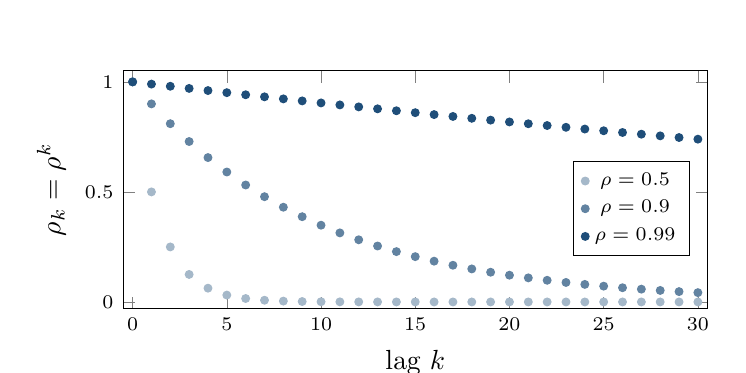
\begin{tikzpicture}
\begin{axis}[width=9cm, height=4.6cm, xmin=-0.5, xmax=30.5, ymin=-0.03, ymax=1.05, xlabel={lag $k$}, ylabel={$\rho_k=\rho^k$},
  tick label style={font=\scriptsize}, legend style={font=\scriptsize, at={(0.97,0.42)}, anchor=east}]
\addplot[only marks, mark=*, mark size=1.4pt, accent!40, domain=0:30, samples=31] {0.5^x};
\addplot[only marks, mark=*, mark size=1.4pt, accent!70, domain=0:30, samples=31] {0.9^x};
\addplot[only marks, mark=*, mark size=1.4pt, accent, domain=0:30, samples=31] {0.99^x};
\legend{$\rho=0.5$,$\rho=0.9$,$\rho=0.99$}
\end{axis}
\end{tikzpicture}
\caption{Autocorrelation functions of AR(1) processes. With $\rho=0.5$ the series forgets its past within a few steps; with $\rho=0.99$ it
remembers for a very long time.}
\end{figure}

\subsection{Forecasting: random walk vs.\ linear extrapolation}
On the 10/9 slides two models are fit to $180$ days of bitcoin log price and asked to forecast $90$ days ahead:
\begin{itemize}[leftmargin=*,itemsep=2pt]
\item \textbf{Linear in time:} fit $Y_t=\beta_0+\beta_1t+\epsilon_t$ and extend the line. The $95\%$ band includes both the noise and the
uncertainty in the fitted line.
\item \textbf{Random walk:} forecast $Y_{t+h}\approx Y_t$ with $95\%$ band $\pm1.96\,\hat\sigma_\epsilon\sqrt h$. Why: unrolling,
$Y_{t+h}=Y_t+\epsilon_{t+1}+\cdots+\epsilon_{t+h}$, a sum of $h$ independent noises with total variance $h\sigma_\epsilon^2$.
\end{itemize}
The linear trend confidently extrapolates whatever trend the last 180 days happened to have, and it was badly wrong when the market turned.
The random-walk band widens like $\sqrt h$ and honestly reflects that the future is uncertain.

\subsection{Prices vs.\ log prices (optional)}
So far $Y_t=\log P_t$. If the log price is (close to) a random walk, $Y_{t+1}=Y_t+\epsilon_{t+1}$, then exponentiating,
\[
P_{t+1}=e^{Y_{t+1}}=e^{Y_t}e^{\epsilon_{t+1}}=P_t\,e^{\epsilon_{t+1}}\approx P_t(1+\epsilon_{t+1}).
\]
The last step is the tangent-line approximation $e^x\approx1+x$ for small $x$ (the derivative of $e^x$ at $0$ is $1$). So each day the
price is \emph{multiplied} by a random factor: a \textbf{multiplicative process}. Then $P_{t+1}-P_t\approx P_t\,\epsilon_{t+1}$: the daily
change is proportional to the current price. The relative volatility is constant ($\hat\sigma_\epsilon\approx0.04$ in natural log, about
$4\%$ a day; this is the $0.016$ above times $\ln10$), but in dollars the swings grow with the price: a typical daily move was about \$3 in
2015 and about \$900 in the last year.

%==========================================================
\section{Study design and multiple predictors (Unit 4.1--4.2)}\label{sec:mult}
%==========================================================
\subsection{Two ways to collect data}
Does a treatment ($X=1$) change an outcome $Y$, compared with no treatment ($X=0$)?

\begin{center}
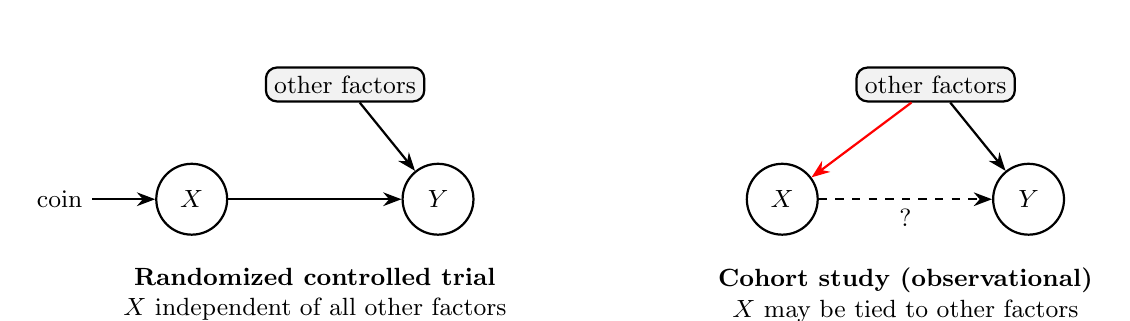
\begin{tikzpicture}[node distance=2.2cm, every node/.style={font=\small},
  var/.style={circle, draw, thick, minimum size=0.9cm}, fac/.style={rounded corners, draw, thick, fill=gray!10, inner sep=3pt}]
\node[var] (X1) {$X$};
\node[var, right=2.2cm of X1] (Y1) {$Y$};
\node[fac, above right=0.9cm and 0.6cm of X1] (F1) {other factors};
\node[left=0.8cm of X1] (coin) {coin};
\draw[-{Stealth}, thick] (coin) -- (X1);
\draw[-{Stealth}, thick] (X1) -- (Y1);
\draw[-{Stealth}, thick] (F1) -- (Y1);
\node[below=0.75cm of $(X1)!0.5!(Y1)$, align=center] {\textbf{Randomized controlled trial}\\ $X$ independent of all other factors};
\begin{scope}[xshift=7.5cm]
\node[var] (X2) {$X$};
\node[var, right=2.2cm of X2] (Y2) {$Y$};
\node[fac, above right=0.9cm and 0.6cm of X2] (F2) {other factors};
\draw[-{Stealth}, thick, dashed] (X2) -- node[below] {?} (Y2);
\draw[-{Stealth}, thick] (F2) -- (Y2);
\draw[-{Stealth}, thick, red] (F2) -- (X2);
\node[below=0.75cm of $(X2)!0.5!(Y2)$, align=center] {\textbf{Cohort study (observational)}\\ $X$ may be tied to other factors};
\end{scope}
\end{tikzpicture}
\end{center}
\begin{itemize}[leftmargin=*,itemsep=2pt]
\item \textbf{Randomized controlled trial (RCT):} we assign $X$ by a coin flip, so $X$ is independent of every other factor, measured or not.
Any difference in $Y$ between the groups must come from $X$.
\item \textbf{Cohort study:} we follow people and observe who gets $X$. Then $X$ may be correlated with other factors that also affect $Y$
(the red arrow), and we cannot tell what causes what. Such a factor is a \textbf{confounder}.
\end{itemize}
For most questions in the social sciences an RCT is impossible. Multiple regression is the main tool for \emph{controlling} for the
confounders we can measure.

\subsection{Example: children's test scores}
$N=434$ children. $Y$: the child's test score; $X_{hs}=1$ if the mother finished high school ($0$ if not); $X_{iq}$: the mother's IQ.
(IQ is an imperfect measure of cognitive ability: one test score that also depends on the test, the conditions, and the person's background.)

Standard deviations: $\sigma_Y=20.4$, $\sigma_{HS}=0.41$, $\sigma_{IQ}=15$. We write $\beta'$ (with a prime) for a \emph{single-predictor}
coefficient, to distinguish it from the coefficients $\beta$ of the two-predictor model.
\begin{itemize}[leftmargin=*,itemsep=2pt]
\item $Y$ on $X_{hs}$: $\hat\beta'_{hs}=11.8$ (the difference in average score between the two groups), $\hat\rho=\hat\beta'_{hs}\sigma_{HS}/\sigma_Y\approx0.24$.
\item $Y$ on $X_{iq}$: $\hat\beta'_{iq}=0.61$, $\hat\rho=\hat\beta'_{iq}\sigma_{IQ}/\sigma_Y\approx0.45$.
\item Mothers who finished high school have higher average IQ: $102.2$ vs.\ $91.9$.
\end{itemize}

\subsection{What we computed vs.\ what we want}
\begin{itemize}[leftmargin=*,itemsep=2pt]
\item \textbf{Computed from the single-predictor regression:} the difference in average score between the groups,
$\beta'_{hs}=\E[Y\given X_{hs}=1]-\E[Y\given X_{hs}=0]$ ($\hat\beta'_{hs}=11.8$). Part of this is really an IQ difference.
\item \textbf{What we want:} the difference \emph{with IQ held fixed},
$\beta_{hs}=\E[Y\given X_{hs}=1,X_{iq}=x]-\E[Y\given X_{hs}=0,X_{iq}=x]$.
\item To compare children whose mothers have the same IQ, put both variables in the model:
\[
Y=\beta_0+\beta_{hs}X_{hs}+\beta_{iq}X_{iq}+\epsilon,\qquad\epsilon\sim\Norm(0,\sigma_\epsilon^2).
\]
\end{itemize}
Fitting it in Python with statsmodels:
\begin{lstlisting}
import statsmodels.api as sm

X = sm.add_constant(np.column_stack([mom_hs, mom_iq]))
results = sm.OLS(kid_score, X).fit()
print(results.summary())
\end{lstlisting}
\begin{lstlisting}[style=output]
Dep. Variable:                      y   R-squared:                       0.214
No. Observations:                 434   Adj. R-squared:                  0.210
==============================================================================
                 coef    std err          t      P>|t|      [0.025      0.975]
------------------------------------------------------------------------------
const         25.7315      5.875      4.380      0.000      14.184      37.279
mom_hs         5.9501      2.212      2.690      0.007       1.603      10.297
mom_iq         0.5639      0.061      9.309      0.000       0.445       0.683
\end{lstlisting}
The \py{coef} column has the least squares estimates $\hat\beta_0=25.7$, $\hat\beta_{hs}=5.95$, $\hat\beta_{iq}=0.56$ (\py{add\_constant}
adds the intercept). \py{std err} is $\se(\hat\beta_k)$, \py{t} is $\hat T=\hat\beta_k/\se$, \py{P>|t|} is the $p$-value, and the last two
columns are the $95\%$ CI (all $t$-based). Controlling for IQ, finishing high school goes with $5.95$ more points, about half of $11.8$.

\subsection{From two predictors to one}
\begin{figure}[h]
\centering
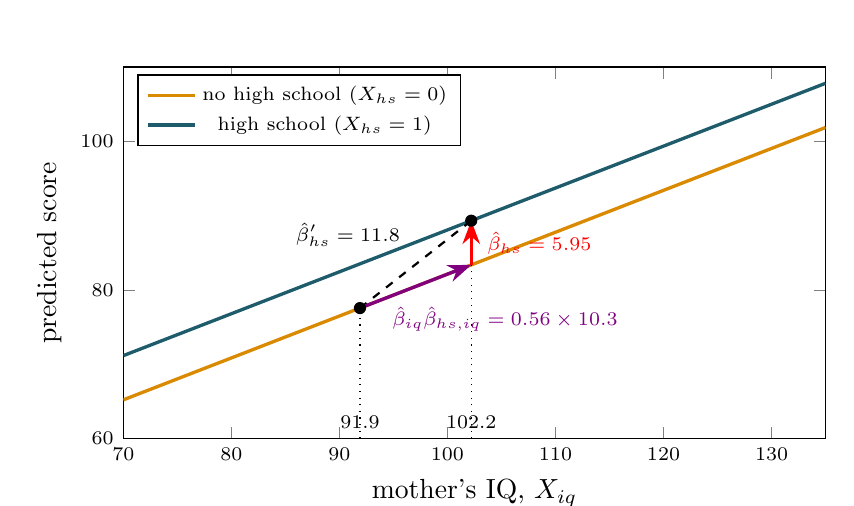
\begin{tikzpicture}
\begin{axis}[width=10.5cm, height=6.3cm, xmin=70, xmax=135, ymin=60, ymax=110, xlabel={mother's IQ, $X_{iq}$}, ylabel={predicted score},
  tick label style={font=\scriptsize}, legend style={font=\scriptsize, at={(0.02,0.98)}, anchor=north west}]
\addplot[hsclr, very thick, domain=70:135] {25.73+0.5639*x};
\addplot[dataclr, very thick, domain=70:135] {25.73+5.95+0.5639*x};
\legend{no high school ($X_{hs}=0$), high school ($X_{hs}=1$)}
\addplot[black, dashed, thick] coordinates {(91.9,77.55) (102.2,89.31)};
\draw[-{Stealth}, violet, very thick] (axis cs:91.9,77.55) -- (axis cs:102.2,83.36);
\draw[-{Stealth}, red, very thick] (axis cs:102.2,83.36) -- (axis cs:102.2,89.31);
\fill (axis cs:91.9,77.55) circle (2.2pt);
\fill (axis cs:102.2,89.31) circle (2.2pt);
\node[font=\scriptsize, anchor=north west, violet] at (axis cs:94,79) {$\hat\beta_{iq}\hat\beta_{hs,iq}=0.56\times10.3$};
\node[font=\scriptsize, anchor=west, red] at (axis cs:102.8,86.3) {$\hat\beta_{hs}=5.95$};
\node[font=\scriptsize, anchor=south east] at (axis cs:96.5,84.5) {$\hat\beta'_{hs}=11.8$};
\draw[dotted] (axis cs:91.9,60) -- (axis cs:91.9,77.55);
\draw[dotted] (axis cs:102.2,60) -- (axis cs:102.2,83.36);
\node[font=\scriptsize, anchor=south] at (axis cs:91.9,60) {91.9};
\node[font=\scriptsize, anchor=south] at (axis cs:102.2,60) {102.2};
\end{axis}
\end{tikzpicture}
\caption{The fitted two-predictor model is two parallel lines (slope $\hat\beta_{iq}$, gap $\hat\beta_{hs}$). The dots are the two groups'
averages. Going from the no-high-school average to the high-school average, the total rise $\hat\beta'_{hs}$ is a move along the line
(purple: the IQ difference times the IQ slope) plus a jump between lines (red: the schooling effect with IQ fixed).}
\end{figure}

Pick a mom without high school (IQ $=a$) and one with (IQ $=b$). The model says their children's expected scores differ by
$\beta_{hs}+\beta_{iq}(b-a)$: the schooling effect plus the IQ difference times the IQ slope. Averaging over all moms in each group replaces
$a$ and $b$ by the group-average IQs:
\[
\underbrace{\E[Y\given X_{hs}{=}1]-\E[Y\given X_{hs}{=}0]}_{\beta'_{hs}}
=\beta_{hs}+\beta_{iq}\underbrace{\big(\E[X_{iq}\given X_{hs}{=}1]-\E[X_{iq}\given X_{hs}{=}0]\big)}_{\beta_{hs,iq}}.
\]
Here $\beta_{hs,iq}$ is the slope when IQ is regressed on schooling. With the numbers: $11.8=5.95+0.56\times10.3$ (the right side is $11.76$).
We say $\beta_{hs}$ is the effect of schooling \textbf{controlling for} IQ (and vice versa). Section~\ref{sec:ovb} proves this decomposition in general.

\subsection{Which predictor matters more?}
$\hat\beta_{hs}=5.95$ is ten times $\hat\beta_{iq}=0.56$, but they have different units (points for finishing high school vs.\ points per IQ
point), so comparing them directly is meaningless. Instead compare the change in average score for a \emph{typical} change in each
predictor, one standard deviation:
\begin{keybox}[title={Scaled coefficients}]
To compare predictors with different units, compare $\hat\beta_k\,\sigma_{X_k}$ (the effect of a one-SD change in $X_k$).
\inwords{multiply each coefficient by its predictor's standard deviation to get ``points of $Y$ per typical change in $X_k$''; these are comparable across predictors.}
\end{keybox}
\begin{lstlisting}
b = results.params
print(b[1] * np.std(mom_hs))   # high school -> 2.441
print(b[2] * np.std(mom_iq))   # IQ          -> 8.449
\end{lstlisting}
A one-SD difference in IQ ($15$ points) goes with about $8.4$ more points; one SD in schooling ($0.41$) with only about $2.4$. IQ matters more.
(The same scaling applies to the CIs: the high-school CI $[1.6,10.3]$ becomes about $[0.66,4.2]$.)

\subsection{$R^2$ with multiple predictors}
$R^2$ is defined exactly as before, $R^2=1-\SSR/\SST$, where now the fitted value $\hat Y_i=\hat\beta_0+\hat\beta_1X_{1,i}+\cdots+\hat\beta_KX_{K,i}$
uses all $K$ predictors ($X_{k,i}$ is the value of predictor $k$ for data point $i$), and $\SSR=\sum_i(Y_i-\hat Y_i)^2$. It is the fraction of
the variation in $Y$ explained by all the predictors together: $R^2\approx1-\Var(Y\given X_1,\dots,X_K)/\Var(Y)$.

\begin{center}
\begin{tabular}{@{}lc@{}}
\toprule
predictors & $R^2$\\\midrule
high school only & 0.06\\
IQ only & 0.20\\
high school and IQ & 0.21\\
\bottomrule
\end{tabular}
\end{center}
\begin{itemize}[leftmargin=*,itemsep=2pt]
\item Adding a predictor never decreases $R^2$ (proved in Section~\ref{sec:ovb}).
\item The $R^2$'s do not add up ($0.06+0.20>0.21$): mothers who finished high school also tend to have higher IQs, so much of what schooling
explains is already explained by IQ.
\item About $79\%$ of the variation is \emph{not} explained: scores have SD $20$ and the residuals still have $\hat\sigma_\epsilon\approx18$.
The model says little about any individual child's score.
\end{itemize}

\begin{examplebox}[title={Question (10/12): midterm scores, difficulty, and QSS}]
$N=64$ students. $y$ = midterm score (fraction of points), \py{difficult} $=1$ if the student rated difficulty 4 (the highest) in the week 1
survey, \py{QSS} $=1$ for QSS majors. Fit: $\hat\beta_0=0.8705$, $\hat\beta_{diff}=-0.1002$ (se $0.040$), $\hat\beta_{QSS}=-0.1340$ (se $0.040$);
\py{np.std(difficult)} $=0.498$, \py{np.std(QSS)} $=0.499$. The joint proportions are:
\begin{center}
\begin{tabular}{lccc}
\toprule
 & \py{difficult}$=0$ & \py{difficult}$=1$ & total\\\midrule
\py{QSS}$=0$ & 0.281 & 0.188 & 0.469\\
\py{QSS}$=1$ & 0.266 & 0.266 & 0.531\\\midrule
total & 0.547 & 0.453 & 1\\
\bottomrule
\end{tabular}
\end{center}
\textbf{Which predictor is more important?} Both are 0/1 with SD $\approx0.5$, so scaling barely changes anything:
$\hat\beta_{diff}\sigma_{diff}=-0.100\times0.498=-0.050$, $\hat\beta_{QSS}\sigma_{QSS}=-0.134\times0.499=-0.067$. QSS is (slightly) more important;
here comparing the raw coefficients would have given the same answer.

\textbf{Single-predictor coefficient of difficulty.} Use $\beta'_{diff}=\beta_{diff}+\beta_{QSS}\,\beta_{diff,QSS}$, where $\beta_{diff,QSS}$
is the slope of QSS on difficulty, a difference of conditional means read off the table (divide a cell by its column total):
\[
\hat\beta_{diff,QSS}=\E[X_{QSS}\given X_{diff}{=}1]-\E[X_{QSS}\given X_{diff}{=}0]=\frac{0.266}{0.453}-\frac{0.266}{0.547}=0.587-0.486=0.101,
\]
so $\hat\beta'_{diff}=-0.100+(-0.134)(0.101)=-0.114$. Fitting $y$ on \py{difficult} alone gives $-0.1137$, as predicted.
\end{examplebox}

%==========================================================
\section{Omitted-variable bias and Simpson's paradox}\label{sec:ovb}
%==========================================================
\subsection{The theorem}
\begin{keybox}[title={Theorem}]
Suppose $Y=\beta_0+\beta_1X_1+\beta_2X_2+\epsilon$, where $\epsilon$ is uncorrelated with $X_1$ and $X_2$, and let $\rho^2=1-\sigma_\epsilon^2/\sigma_Y^2$.
\begin{enumerate}[leftmargin=*,itemsep=2pt,label=(\arabic*)]
\item \textbf{Omitted-variable bias:} if $X_2$ is left out, the slope of the regression of $Y$ on $X_1$ is
\[
\beta'_1=\beta_1+\beta_2\,\beta_{1,2},\qquad \beta_{1,2}=\frac{\Cov(X_1,X_2)}{\Var(X_1)}\quad\text{(the slope of $X_2$ regressed on $X_1$).}
\]
\item Adding a predictor never decreases $\rho^2$.
\end{enumerate}
The same argument with sample covariances shows $R^2$ never decreases. Both results extend to $K$ predictors
(Section~\ref{sec:ovbk}).
\inwords{(1) leaving $X_2$ out makes $X_1$'s slope absorb $X_2$'s effect, scaled by how much $X_2$ rises with $X_1$; (2) adding a predictor can never explain less of $Y$'s variance.}
\end{keybox}
\textbf{Reading (1).} Leaving $X_2$ out does not make its effect disappear; it gets credited to $X_1$, in proportion to how much $X_2$ moves with
$X_1$. The bias $\beta_2\beta_{1,2}$ is zero only if $X_2$ has no effect ($\beta_2=0$) or is uncorrelated with $X_1$ ($\beta_{1,2}=0$). The second
case is exactly what randomization guarantees in an RCT.

\textbf{Proof of (1).} For simplicity assume $X_1,X_2$ have mean zero and all intercepts are zero. The single-predictor slope is
$\beta_1'=\Cov(X_1,Y)/\Var(X_1)$. Using bilinearity of covariance and $\Cov(X_1,\epsilon)=0$:
\begin{align*}
\Cov(X_1,Y)&=\Cov(X_1,\ \beta_1X_1+\beta_2X_2+\epsilon) \why{substitute the model}\\
&=\beta_1\Cov(X_1,X_1)+\beta_2\Cov(X_1,X_2)+\Cov(X_1,\epsilon) \why{bilinearity}\\
&=\beta_1\Var(X_1)+\beta_2\Cov(X_1,X_2). \why{$\Cov(X_1,X_1)=\Var X_1$, $\Cov(X_1,\epsilon)=0$}
\end{align*}
Dividing by $\Var(X_1)$: $\ \beta'_1=\beta_1+\beta_2\dfrac{\Cov(X_1,X_2)}{\Var(X_1)}=\beta_1+\beta_2\beta_{1,2}$. $\square$

\textbf{Proof of (2).} The coefficients of determination of the two- and one-predictor models are
\[
\rho^2=1-\frac{\Var(Y\given X_1,X_2)}{\sigma_Y^2},\qquad \rho'^2=1-\frac{\Var(Y\given X_1)}{\sigma_Y^2},
\]
so we just need $\Var(Y\given X_1)\ge\Var(Y\given X_1,X_2)$. Knowing both predictors, the only randomness left is the noise:
$\Var(Y\given X_1,X_2)=\sigma_\epsilon^2$. Knowing only $X_1$, both $X_2$ and $\epsilon$ are still random; $\beta_1X_1$ is then a constant, and
since $\epsilon$ is independent of $X_1,X_2$ the variances add:
\[
\Var(Y\given X_1)=\Var(\beta_2X_2+\epsilon\given X_1)=\beta_2^2\Var(X_2\given X_1)+\sigma_\epsilon^2\ \ge\ \sigma_\epsilon^2. \qquad\square
\]
In words: more information can only leave less unexplained variance (or the same, if the new predictor is useless).

\textbf{Picture.} With two continuous predictors the model is a plane over the $(x_1,x_2)$ plane. Moving one unit in $x_1$ with $x_2$ fixed raises
$y$ by $\beta_1$. But in the data, when $x_1$ goes up by one, $x_2$ typically goes up by $\beta_{1,2}$ too (the points cluster along the line
$x_2=\beta_{1,2}x_1$), adding another $\beta_2\beta_{1,2}$. The single-predictor slope $\beta'_1$ is the slope of the plane \emph{along that line}.

\begin{examplebox}[title={Question (10/14): poverty, single-parent households, and violent crime}]
50 US states (2009). $Y$: violent crimes per 100{,}000; $X_{pov}$: \% below the poverty line; $X_{single}$: \% of family households headed by a
single parent. Three fits:
\begin{center}
\begin{tabular}{lccc}
\toprule
model & coefficient on poverty & coefficient on single & $R^2$\\\midrule
poverty only & $15.97$ (se $7.19$, $p=0.031$) & --- & 0.093\\
single only & --- & $29.99$ (se $4.92$, $p<0.001$) & 0.436\\
both & $-1.29$ (se $6.57$, $p=0.845$) & $30.54$ (se $5.70$, $p<0.001$) & 0.437\\
\bottomrule
\end{tabular}
\end{center}
\textbf{Interpretation.} Alone, poverty looks associated with crime (16 more crimes per 100{,}000 per percentage point). Controlling for
single-parent households, that association vanishes (the coefficient is near zero with a CI containing 0), while the single-parent coefficient
barely changes. States with more poverty have more single-parent households; the poverty-only regression was picking up the single-parent effect.
(This is an observational study, so these are associations, not causes.)

\textbf{Find $\beta_{pov,single}$.} Use OVB with $X_1=$ poverty, $X_2=$ single: $\beta'_{pov}=\beta_{pov}+\beta_{single}\beta_{pov,single}$, so
\[
15.97=-1.29+30.54\,\hat\beta_{pov,single}\ \Longrightarrow\ \hat\beta_{pov,single}=\frac{15.97+1.29}{30.54}=0.565.
\]
The other way around, $\beta'_{single}=\beta_{single}+\beta_{pov}\beta_{single,pov}$: $29.99=30.54-1.29\,\hat\beta_{single,pov}$, so
$\hat\beta_{single,pov}=0.55/1.29=0.425$.

\textbf{The correlation between the predictors.} Multiply the two slopes:
\[
\beta_{pov,single}\,\beta_{single,pov}=\frac{\Cov}{\Var(X_{pov})}\cdot\frac{\Cov}{\Var(X_{single})}=\left(\frac{\Cov}{\sigma_{pov}\sigma_{single}}\right)^2=\rho^2,
\]
so $\hat\rho=\sqrt{0.565\times0.425}=\sqrt{0.240}=0.49$ (positive, since both slopes are positive).
\end{examplebox}

\subsection{Simpson's paradox}
\begin{center}
\begin{tabular}{@{}lccc@{}}
\toprule
 & 1995 & 1996 & both years\\\midrule
Derek Jeter & $12/48=.250$ & $183/582=.314$ & $195/630=.310$\\
David Justice & $104/411=.253$ & $45/140=.321$ & $149/551=.270$\\
\bottomrule
\end{tabular}
\end{center}
Batting average $=$ hits / at bats. Justice has the higher average \emph{in each year}, but Jeter has the higher average \emph{overall}.
This reversal is \textbf{Simpson's paradox}.

\begin{examplebox}[title={Question (10/14): explain it with omitted-variable bias}]
Let $Y=1$ for a hit (0 otherwise), $X_{jeter}=1$ for Jeter (0 for Justice), $X_{year}=1$ for 1996 (0 for 1995), and consider
$\E[Y\given X_{jeter},X_{year}]=\beta_0+\beta_{jeter}X_{jeter}+\beta_{year}X_{year}$. Matching the four cells of the table:
\begin{align*}
\beta_0&\approx\E[Y\given X_{jeter}{=}0,X_{year}{=}0]=104/411=.253,\\
\beta_0+\beta_{jeter}&\approx\E[Y\given X_{jeter}{=}1,X_{year}{=}0]=12/48=.250,\\
\beta_0+\beta_{year}&\approx\E[Y\given X_{jeter}{=}0,X_{year}{=}1]=45/140=.321,\\
\beta_0+\beta_{jeter}+\beta_{year}&\approx\E[Y\given X_{jeter}{=}1,X_{year}{=}1]=183/582=.314.
\end{align*}
Only approximately: four averages cannot be matched exactly by three $\beta$'s (that needs an \emph{interaction} term
$\beta_{int}X_{jeter}X_{year}$, coming soon). Reading off differences, $\hat\beta_{jeter}\approx-0.006$ (Justice is slightly better in both
years) and $\hat\beta_{year}\approx0.067$ (everyone hit better in 1996).

\textbf{The omitted variable is the year.} The table also gives how the year depends on the player:
$\E[X_{year}\given X_{jeter}{=}1]=582/630=.924$ and $\E[X_{year}\given X_{jeter}{=}0]=140/551=.254$, so
$\hat\beta_{jeter,year}=.924-.254=.670$: almost all of Jeter's at bats came in the good year. By OVB,
\[
\hat\beta'_{jeter}=\hat\beta_{jeter}+\hat\beta_{year}\,\hat\beta_{jeter,year}=-0.006+0.067\times0.670=0.039,
\]
matching the overall difference $.310-.270=.040$. A small negative direct effect is swamped by a large positive omitted-variable term.
\end{examplebox}

\textbf{Other examples of Simpson's paradox} (each is OVB with a confounder):
\begin{itemize}[leftmargin=*,itemsep=2pt]
\item \textbf{UC Berkeley graduate admissions, 1973:} men admitted at a higher rate overall (44\% vs.\ 35\%), but in most departments women were
admitted at a similar or higher rate. Omitted variable: department; women applied more often to departments that admitted few applicants.
\item \textbf{Kidney stones:} open surgery succeeded more often than a newer procedure for small stones (93\% vs.\ 87\%) and for large stones
(73\% vs.\ 69\%), but less often overall (78\% vs.\ 83\%). Omitted variable: stone size; open surgery was used mostly on the harder, large stones.
\item \textbf{Smoking and survival (Whickham, UK):} over 20 years a higher fraction of smokers than non-smokers survived (76\% vs.\ 69\%), but
within most age groups smokers died at higher rates. Omitted variable: age; the smokers were younger.
\item \textbf{COVID-19, early 2020:} the case fatality rate was higher in Italy than in China overall, but lower in every age group.
Omitted variable: age; Italy's cases were older.
\end{itemize}

\begin{examplebox}[title={Question (10/14): regressing an AR(1) on two lags}]
For a stationary AR(1) with coefficient $\rho$, fit $Y_t=\beta_0+\beta_{lag1}Y_{t-1}+\beta_{lag2}Y_{t-2}+\epsilon$. What are $\beta_{lag1}$ and
$\beta_{lag2}$? What if we regress $Y_t$ on $Y_{t-2}$ alone?

\textbf{Two lags:} the AR(1) model says that once $Y_{t-1}$ is known, $Y_{t-2}$ tells us nothing more about $Y_t$, so $\beta_{lag1}=\rho$ and
$\beta_{lag2}=0$.

\textbf{$Y_{t-2}$ alone:} $\beta'_{lag2}=\Cov(Y_{t-2},Y_t)/\sigma_Y^2=\rho_2=\rho^2$ (autocorrelation at lag 2). OVB gives the same answer:
leaving out $Y_{t-1}$, $\beta'_{lag2}=\beta_{lag2}+\beta_{lag1}\cdot(\text{slope of }Y_{t-1}\text{ on }Y_{t-2})=0+\rho\cdot\rho=\rho^2$.
Yesterday's effect gets credited to the day before yesterday.
\end{examplebox}

%==========================================================
\section{Omitted variables in AR processes (Lecture 15)}\label{sec:arovb}
%==========================================================
The omitted-variable bias formula also explains what happens when a time series is regressed on too few (or too many) of its own past
values. Throughout, the process is stationary (Section~\ref{sec:ar}): every $Y_t$ has the same mean and variance, and the covariance of
$Y_t$ and $Y_{t-k}$ depends only on the gap $k$. So the slope of $Y_{t-1}$ on $Y_{t-k}$ equals the slope of $Y_t$ on $Y_{t-k+1}$.

\begin{examplebox}[title={Question (10/19): an AR(1) fit with extra lags, and with lag $k$ alone}]
Data come from $Y_t=\rho Y_{t-1}+\epsilon_t$ (stationary), and we fit $Y_t=\beta_0+\beta_1Y_{t-1}+\beta_2Y_{t-2}+\epsilon'_t$. With lots of data,
what are $\hat\beta_1,\hat\beta_2$? What is the slope when $Y_{t-1}$ is left out? What is the slope of $Y_t$ on $Y_{t-k}$ alone?

\textbf{Two lags.} The true model already has the form of the fitted one, with $\beta_1=\rho$, $\beta_2=0$, and $\epsilon_t$ uncorrelated with
the past values $Y_{t-1},Y_{t-2}$. So $\hat\beta_1\to\rho$ and $\hat\beta_2\to0$: once yesterday is known, the day before adds nothing.

\textbf{Leave out $Y_{t-1}$.} OVB with $X_1=Y_{t-2}$ (kept) and $X_2=Y_{t-1}$ (left out):
$\beta'_{lag2}=\underbrace{0}_{\beta_{lag2}}+\underbrace{\rho}_{\beta_{lag1}}\cdot\underbrace{\rho}_{\text{slope of }Y_{t-1}\text{ on }Y_{t-2}}=\rho^2$.

\textbf{Lag $k$ alone.} Fit $Y_t$ on $Y_{t-1}$ and $Y_{t-k}$: the true coefficients are $\rho$ and $0$. Leaving out $Y_{t-1}$,
\[
\beta'_{lag\,k}=0+\rho\cdot(\text{slope of }Y_{t-1}\text{ on }Y_{t-k})=\rho\cdot\beta'_{lag\,k-1}.
\]
The slope of $Y_{t-1}$ on $Y_{t-k}$ is a gap of $k-1$ steps, which by stationarity is $\beta'_{lag\,k-1}$. Starting from $\beta'_{lag1}=\rho$ and
multiplying by $\rho$ each step gives $\beta'_{lag\,k}=\rho^k$, the autocorrelation $\rho_k$ from Section~\ref{sec:ar}. Each step back multiplies the
effect by another $\rho$.
\end{examplebox}

\begin{examplebox}[title={Question (10/19): an AR(2) process fit with one lag}]
Now $Y_t=0.5\,Y_{t-1}+0.3\,Y_{t-2}+\epsilon_t$, $\epsilon_t\sim\Norm(0,1)$. In the slides' simulation it looks much like an AR(1) with $\rho=0.8$
(slow, wandering swings). What is the slope of the single-predictor regression of $Y_t$ on $Y_{t-1}$, with $Y_{t-2}$ left out?

\textbf{OVB.} $X_1=Y_{t-1}$ (kept), $X_2=Y_{t-2}$ (left out):
$\beta'_{lag1}=0.5+0.3\,\beta_{1,2}$, where $\beta_{1,2}$ is the slope of $Y_{t-2}$ on $Y_{t-1}$. By stationarity that is a one-step slope,
$\Cov(Y_{t-1},Y_{t-2})/\sigma_Y^2=\rho_1$, the lag-1 autocorrelation.

\textbf{Find $\rho_1$.} The single-predictor slope we want is also a one-step slope, so $\beta'_{lag1}=\rho_1$ too. Directly:
\begin{align*}
\Cov(Y_t,Y_{t-1})&=\Cov(0.5Y_{t-1}+0.3Y_{t-2}+\epsilon_t,\ Y_{t-1}) \why{substitute the model}\\
&=0.5\,\sigma_Y^2+0.3\,\Cov(Y_{t-2},Y_{t-1})+0 \why{bilinearity; $\epsilon_t$ is new noise}\\
\rho_1&=0.5+0.3\,\rho_1 \why{divide by $\sigma_Y^2$; stationarity}\\
\rho_1&=\frac{0.5}{0.7}=\frac57\approx0.714. \why{solve}
\end{align*}
So $\beta'_{lag1}=0.5+0.3\times0.714=0.714$. The single-lag slope ($0.71$) is bigger than the true lag-1 coefficient ($0.5$) because it also
picks up the effect of $Y_{t-2}$, which moves with $Y_{t-1}$.
\end{examplebox}

\subsection{Real series: AR($k$) fits with $k=1,\dots,10$}
The slides fit each series on its previous $k$ values for $k=1,\dots,10$ and plot $R^2$ and the coefficients against $k$:
\begin{itemize}[leftmargin=*,itemsep=2pt]
\item \textbf{Bitcoin} ($Y_t=\log_{10}$ daily price, 4283 days). $R^2\approx1$ for every $k$. The lag-1 coefficient stays near 1 (about $0.9$
once more lags are added), and lags $2,\dots,k$ are all near 0. Earlier days add essentially nothing once yesterday's price is known: the
behavior of a random walk (Section~\ref{sec:ar}).
\item \textbf{Daily casualty counts} (Ukraine: Russian personnel losses; Gaza: reported deaths). $R^2$ rises only a little with $k$
(Ukraine about $0.82\to0.86$, Gaza about $0.25\to0.37$), but the lag-1 coefficient falls a lot as lags are added (Ukraine about $0.9\to0.4$,
Gaza about $0.5\to0.3$), and the other lags get positive coefficients. These series are \emph{not} AR(1): several past days matter. With only
lag 1 in the model, its coefficient absorbs the effects of the omitted earlier days, which is OVB exactly as in the AR(2) question.
\end{itemize}

%==========================================================
\section{Categorical predictors: the incumbency advantage (Lecture 15, Unit 4.5)}\label{sec:cat}
%==========================================================
\subsection{The data and a first model}
How big is the advantage of already holding the seat? US House elections, 435 districts (from \emph{Regression and Other Stories}):
\begin{itemize}[leftmargin=*,itemsep=2pt]
\item $Y$ (\py{vote}): Democratic share of the two-party vote in 1988, as a fraction from 0 to 1;
\item $X_{past}$ (\py{past\_vote}): Democratic share in 1986, on the same scale;
\item $X_{inc}$ (\py{inc}): $+1$ if a Democrat is the incumbent, $-1$ if a Republican is, $0$ for an open seat.
\end{itemize}
Uncontested races are set to $0.75$ or $0.25$. Since shares are fractions, a coefficient of $0.1$ means 10 percentage points. In the scatter
plot of 1988 vs.\ 1986 share, the points lie near the line $y=x$, with Democratic incumbents in the upper right, Republican incumbents in the
lower left, and open seats in between.

\begin{examplebox}[title={Question (10/19): a limitation of the model $Y=\beta_0+\beta_{past}X_{past}+\beta_{inc}X_{inc}+\epsilon$}]
Any one of these is a fine answer (all are assumptions, not data problems):
\begin{itemize}[leftmargin=*,itemsep=1pt]
\item Coding $X_{inc}$ as $-1,0,1$ forces the step from a Republican incumbent to an open seat to have the \emph{same} effect as the step from
an open seat to a Democratic incumbent, so the advantage is assumed equal for both parties. (Fixed below with dummy variables.)
\item Incumbency is not randomized. Incumbents may be stronger candidates, or hold seats for reasons the model does not see, so $\beta_{inc}$
is an association controlling for past vote, not necessarily a causal effect.
\item The model is linear in past vote, with the same noise variance for every district.
\item Uncontested races are set to arbitrary values (0.25, 0.75), which affects the fit.
\end{itemize}
\end{examplebox}

\begin{lstlisting}[style=output]
Dep. Variable:                   vote   R-squared:                       0.819
==============================================================================
                 coef    std err          t      P>|t|      [0.025      0.975]
------------------------------------------------------------------------------
const          0.5063      0.004    121.695      0.000       0.498       0.514
inc            0.1906      0.004     44.210      0.000       0.182       0.199
\end{lstlisting}
\begin{lstlisting}[style=output]
Dep. Variable:                   vote   R-squared:                       0.887
==============================================================================
                 coef    std err          t      P>|t|      [0.025      0.975]
------------------------------------------------------------------------------
const          0.2380      0.017     14.068      0.000       0.205       0.271
past_vote      0.5210      0.032     16.169      0.000       0.458       0.584
inc            0.0964      0.007     14.284      0.000       0.083       0.110
\end{lstlisting}

\begin{examplebox}[title={Question (10/19): interpret, recover a slope with OVB, and compare importance}]
\textbf{Interpret.} \emph{Inc only:} districts one step apart in incumbency (Republican incumbent $\to$ open $\to$ Democratic incumbent) differ
by $0.19$ (19 points) in average Democratic share. This mixes two things: incumbency, and the fact that Democratic incumbents hold districts
that already vote Democratic. \emph{With past vote:} comparing districts with the \emph{same} 1986 share, one step of incumbency goes with
$0.096$, about 10 points. A Democratic vs.\ a Republican incumbent (two steps) is about 19 points.

\textbf{Slope of past vote on inc.} OVB with $X_1=$ inc (kept) and $X_2=$ past vote (left out), $\beta'_{inc}=\beta_{inc}+\beta_{past}\beta_{inc,past}$:
\[
0.1906=0.0964+0.521\,\hat\beta_{inc,past}\ \Longrightarrow\ \hat\beta_{inc,past}=\frac{0.0942}{0.521}\approx0.18.
\]
One step in incumbency goes with 18 points more Democratic vote in 1986. Check: a slope is $\rho\,\sigma_{past}/\sigma_{inc}=0.86\times0.20/0.95=0.18$
(using the correlation $0.86$ from Section~\ref{sec:collin}).

\textbf{Which matters more?} Scale by the SDs $\sigma_{past}\approx0.20$, $\sigma_{inc}\approx0.95$:
$\hat\beta_{past}\sigma_{past}=0.521\times0.20=0.104$ and $\hat\beta_{inc}\sigma_{inc}=0.0964\times0.95=0.092$. They are about equally important,
with past vote slightly ahead (one SD of each moves the expected share by about 10 points). The raw coefficients ($0.52$ vs.\ $0.10$) would
exaggerate the difference.
\end{examplebox}

\subsection{Dummy variables}
\texttt{inc} is really \textbf{categorical}: it names a category (Republican incumbent, open seat, Democratic incumbent) rather than a number on a
scale. Going from a Republican incumbent to an open seat need not have the same effect as going from an open seat to a Democratic incumbent.
To let each category have its own effect, introduce \textbf{dummy variables}, each equal to 1 for one category and 0 otherwise:
$X_{dem}$ (\py{dem\_inc}), $X_{rep}$ (\py{rep\_inc}), $X_{open}$. With all three:
\[
Y=\beta_0+\beta_{past}X_{past}+\beta_{dem}X_{dem}+\beta_{rep}X_{rep}+\beta_{open}X_{open}+\epsilon.
\]

\begin{examplebox}[title={Question (10/19): what is the interpretation of $\beta_{dem}$ in this model?}]
By the usual reading, $\beta_{dem}$ is the change in average $Y$ when $X_{dem}$ goes up by 1 \emph{with the other predictors held fixed}. But every
district is in exactly one category, so $X_{dem}+X_{rep}+X_{open}=1$ always. If $X_{rep}$ and $X_{open}$ are held fixed, $X_{dem}$ cannot change,
so $\beta_{dem}$ has no meaning.

The same problem shows up in the fit. Add any number $c$ to $\beta_{dem},\beta_{rep},\beta_{open}$ and subtract $c$ from $\beta_0$: every prediction
is unchanged (it changes by $c(X_{dem}+X_{rep}+X_{open})-c=0$). The data cannot choose among these, so least squares has no unique answer. The
dummies are \textbf{collinear} with the intercept.
\end{examplebox}

\textbf{Solution: leave one category out}, the \textbf{baseline} (here, open seats). Compare the linear and the categorical models:
\[
Y=\beta_0+\beta_{past}X_{past}+\beta_{inc}X_{inc}+\epsilon,\qquad
Y=\beta_0+\beta_{past}X_{past}+\beta_{dem}X_{dem}+\beta_{rep}X_{rep}+\epsilon.
\]
Now $\beta_{dem}$ is the difference between a Democratic incumbent and an open seat, and $\beta_{rep}$ the difference between a Republican
incumbent and an open seat, each with past vote held fixed.
\begin{lstlisting}[style=output]
Dep. Variable:                   vote   R-squared:                       0.888
==============================================================================
                 coef    std err          t      P>|t|      [0.025      0.975]
------------------------------------------------------------------------------
const          0.2530      0.020     12.947      0.000       0.215       0.291
past_vote      0.5270      0.032     16.260      0.000       0.463       0.591
dem_inc        0.0760      0.015      5.089      0.000       0.047       0.105
rep_inc       -0.1152      0.014     -8.227      0.000      -0.143      -0.088
\end{lstlisting}

\begin{examplebox}[title={Question (10/19): which $\beta_{dem},\beta_{rep}$ give back the linear model? Same advantage for both parties?}]
In the linear model the incumbency term is $\beta_{inc}X_{inc}$, which is $+\beta_{inc}$ for a Democratic incumbent, $-\beta_{inc}$ for a Republican,
and $0$ for an open seat. The dummy model gives $\beta_{dem}$, $\beta_{rep}$, and $0$. They agree when
\[
\beta_{dem}=\beta_{inc},\qquad\beta_{rep}=-\beta_{inc}.
\]
So the linear model is the special case where the two advantages have the same size.

\textbf{Compare.} $\hat\beta_{inc}=0.096$, while $\hat\beta_{dem}=0.076$ and $\hat\beta_{rep}=-0.115$: the estimated advantage is about 8 points for
Democratic incumbents and 12 points for Republican incumbents, and $0.096$ is roughly their average. The CIs are $[0.047,0.105]$ and (in size)
$[0.088,0.143]$, which overlap, so the data do not clearly show the advantages differ. $R^2$ barely moves ($0.887\to0.888$).
\end{examplebox}

\begin{keybox}[title={Dummy variables for a categorical predictor}]
A categorical predictor with $m$ categories enters the model as $m-1$ dummy variables; the left-out category is the \textbf{baseline}.
\begin{itemize}[leftmargin=*,itemsep=1pt]
\item The coefficient on a dummy is the difference in average $Y$ between that category and the baseline, with the other predictors held fixed.
\item The difference between two non-baseline categories $a$ and $b$ is $\beta_a-\beta_b$ (the intercepts cancel).
\item Including all $m$ dummies and an intercept does not work: the dummies add to 1, so they are collinear with the intercept.
\end{itemize}
\inwords{give each category its own 0/1 column except one; each coefficient then measures ``this category vs.\ the left-out one''.}
\end{keybox}

\begin{examplebox}[title={Example (Unit 4.5): earnings disparities between ethnic groups}]
Earnings data (US adults; $Y$ = earnings in \$1000s), with ethnicity in four categories: Black, Hispanic, Other, White. Python drops the first
category alphabetically, so Black is the baseline:
\[
Y=\beta_0+\beta_{hispanic}X_{hispanic}+\beta_{other}X_{other}+\beta_{white}X_{white}+\epsilon.
\]
In terms of conditional expectations, $\beta_{white}=\E[Y\given\text{White}]-\E[Y\given\text{Black}]\approx4.9$ and
$\beta_{hispanic}=\E[Y\given\text{Hispanic}]-\E[Y\given\text{Black}]\approx-0.7$. The White--Hispanic gap is not a single coefficient, but
\begin{align*}
\E[Y\given\text{White}]-\E[Y\given\text{Hispanic}]&=(\beta_0+\beta_{white})-(\beta_0+\beta_{hispanic})\\
&=\beta_{white}-\beta_{hispanic}\approx4.9-(-0.7)=5.6,
\end{align*}
about \$5{,}600.
\begin{lstlisting}
import pandas as pd
D = pd.get_dummies(df["ethnicity"], drop_first=True, dtype=float)
X = sm.add_constant(D)
results = sm.OLS(df["earnk"], X).fit()
\end{lstlisting}
\end{examplebox}

%==========================================================
\section{Leaving out all predictors but one (Lecture 16)}\label{sec:ovbk}
%==========================================================
\subsection{Omitted-variable bias with many predictors}
\begin{keybox}[title={Theorem (OVB for $K$ predictors)}]
Suppose $Y=\beta_0+\beta_1X_1+\beta_2X_2+\cdots+\beta_KX_K+\epsilon$, where $\epsilon$ is uncorrelated with $X_1,\dots,X_K$. If $X_2,\dots,X_K$
are all left out, the slope of the regression of $Y$ on $X_1$ is
\[
\beta'_1=\beta_1+\sum_{j=2}^K\beta_j\,\beta_{1,j},\qquad \beta_{1,j}=\frac{\Cov(X_1,X_j)}{\Var(X_1)}\quad\text{(slope of $X_j$ on $X_1$; the slides write $\beta'_{1,j}$).}
\]
\inwords{the single-predictor slope is the direct effect of $X_1$ plus, for every left-out predictor, (how much it moves with $X_1$) $\times$ (its own effect).}
\end{keybox}

\begin{examplebox}[title={Question (10/21): derive the formula, assuming $\E[X_j]=0$ and $\beta_0=0$ (so $\E[Y]=0$)}]
The single-predictor slope is $\beta'_1=\Cov(X_1,Y)/\Var(X_1)$. Expand the covariance:
\begin{align*}
\Cov(X_1,Y)&=\Cov\Big(X_1,\ \beta_1X_1+\sum_{j=2}^K\beta_jX_j+\epsilon\Big) \why{substitute the model}\\
&=\beta_1\Cov(X_1,X_1)+\sum_{j=2}^K\beta_j\Cov(X_1,X_j)+\Cov(X_1,\epsilon) \why{bilinearity, one term at a time}\\
&=\beta_1\Var(X_1)+\sum_{j=2}^K\beta_j\Cov(X_1,X_j). \why{$\Cov(X_1,\epsilon)=0$}
\end{align*}
Dividing by $\Var(X_1)$ gives $\beta'_1=\beta_1+\sum_{j\ge2}\beta_j\,\Cov(X_1,X_j)/\Var(X_1)=\beta_1+\sum_{j\ge2}\beta_j\beta_{1,j}$. $\square$
(This is the two-predictor proof of Section~\ref{sec:ovb} with $K-1$ omitted terms instead of one.)
\end{examplebox}

\textbf{Picture.} Every path from $X_1$ to $Y$ contributes: the direct arrow ($\beta_1$), and each detour through a left-out $X_j$ (the slope
$\beta_{1,j}$ times the effect $\beta_j$). The single-predictor slope adds up all the paths.
\begin{center}
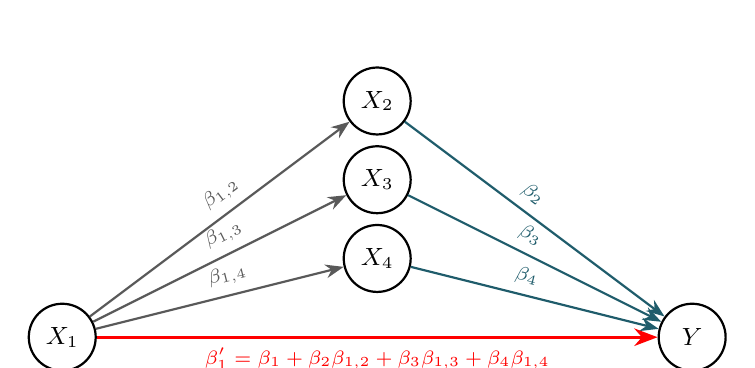
\begin{tikzpicture}[>={Stealth}, every node/.style={font=\small},
  var/.style={circle, draw, thick, minimum size=0.85cm, inner sep=1pt}]
\node[var] (X1) at (0,0) {$X_1$};
\node[var] (Y) at (8,0) {$Y$};
\foreach \j/\y in {2/3.0,3/2.0,4/1.0}{
  \node[var] (X\j) at (4,\y) {$X_\j$};
  \draw[->, thick, gray!70!black] (X1) -- node[sloped, above, pos=0.55, font=\scriptsize] {$\beta_{1,\j}$} (X\j);
  \draw[->, thick, dataclr] (X\j) -- node[sloped, above, pos=0.45, font=\scriptsize] {$\beta_\j$} (Y);
}
\draw[->, very thick, red] (X1) -- node[below, font=\scriptsize] {$\beta'_1=\beta_1+\beta_2\beta_{1,2}+\beta_3\beta_{1,3}+\beta_4\beta_{1,4}$} (Y);
\end{tikzpicture}
\end{center}

\subsection{Example: earnings, gender, and education}
How are earnings related to gender and education, and what else could explain these associations? A survey of 1814 US adults (from
\emph{Regression and Other Stories}); the fits use the 1627 respondents with positive earnings.
\begin{itemize}[leftmargin=*,itemsep=2pt]
\item $Y$: \py{earnk}, earnings in \$1000s. Earnings are strongly right-skewed (a few very large values), so we model $\log(\text{earnk})$.
\item $X_{hispanic},X_{other},X_{white}$: ethnicity dummies, with Black as the baseline.
\item $X_{male}$ (0/1), $X_{height}$ (inches), $X_{educ}$ (years of education), $X_{age}$ (years).
\end{itemize}
\begin{align*}
\log(\text{earnk})=\beta_0&+\beta_{hispanic}X_{hispanic}+\beta_{other}X_{other}+\beta_{white}X_{white}\\
&+\beta_{male}X_{male}+\beta_{height}X_{height}+\beta_{educ}X_{educ}+\beta_{age}X_{age}+\epsilon
\end{align*}
\begin{lstlisting}[style=output]
Dep. Variable:              log_earnk   R-squared:                       0.211
==============================================================================
                 coef    std err          t      P>|t|      [0.025      0.975]
------------------------------------------------------------------------------
const         -0.5156      0.496     -1.039      0.299      -1.489       0.458
hispanic      -0.0355      0.105     -0.337      0.736      -0.242       0.171
other          0.0363      0.152      0.238      0.812      -0.263       0.335
white          0.0845      0.067      1.268      0.205      -0.046       0.215
male           0.4175      0.058      7.222      0.000       0.304       0.531
height         0.0166      0.007      2.223      0.026       0.002       0.031
education      0.1189      0.008     14.885      0.000       0.103       0.135
age            0.0092      0.001      7.724      0.000       0.007       0.012
\end{lstlisting}
\textbf{Reading log coefficients.} The log here is the natural log, as in \emph{Regression and Other Stories}. A coefficient $b$ on $\log Y$
multiplies earnings by $e^b$, and $e^b\approx1+b$ for small $b$ (Section~\ref{sec:ar}, prices vs.\ log prices). So, holding the other
predictors fixed:
\begin{itemize}[leftmargin=*,itemsep=1pt]
\item each extra year of education goes with about $12\%$ higher earnings ($e^{0.119}\approx1.13$);
\item men earn about $e^{0.42}\approx1.52$ times as much as women of the same height, education, age, and ethnicity ($b$ is too big here for $1+b$);
\item an extra inch of height goes with about $1.7\%$ more, and an extra year of age with about $0.9\%$ more;
\item the ethnicity CIs all contain 0: controlling for the rest, there is no clear ethnicity difference in this sample.
\end{itemize}
\textbf{Scaled coefficients} $\hat\beta_j\sigma_j$ put them on one scale: education is the most important ($\approx0.30$), then male ($\approx0.20$)
and age ($\approx0.16$), with height ($\approx0.06$) and ethnicity near 0. The slides also compare $Y=\text{earnk}$ ($R^2=0.18$) with
$Y=\log(\text{earnk})$ ($R^2=0.21$), scaling each coefficient by $\sigma_j/\sigma_Y$: the two give nearly the same picture.

\subsection{Leaving out all predictors but education}
Regress $\log(\text{earnk})$ on education alone: $\hat\beta'_{educ}\approx0.115$, barely different from $\hat\beta_{educ}\approx0.119$. The theorem says
exactly why. Here $\beta_{educ,j}$ is the slope of each other predictor on education (left arrows), and $\beta_j$ is its coefficient in the full
model (right arrows):
\begin{center}
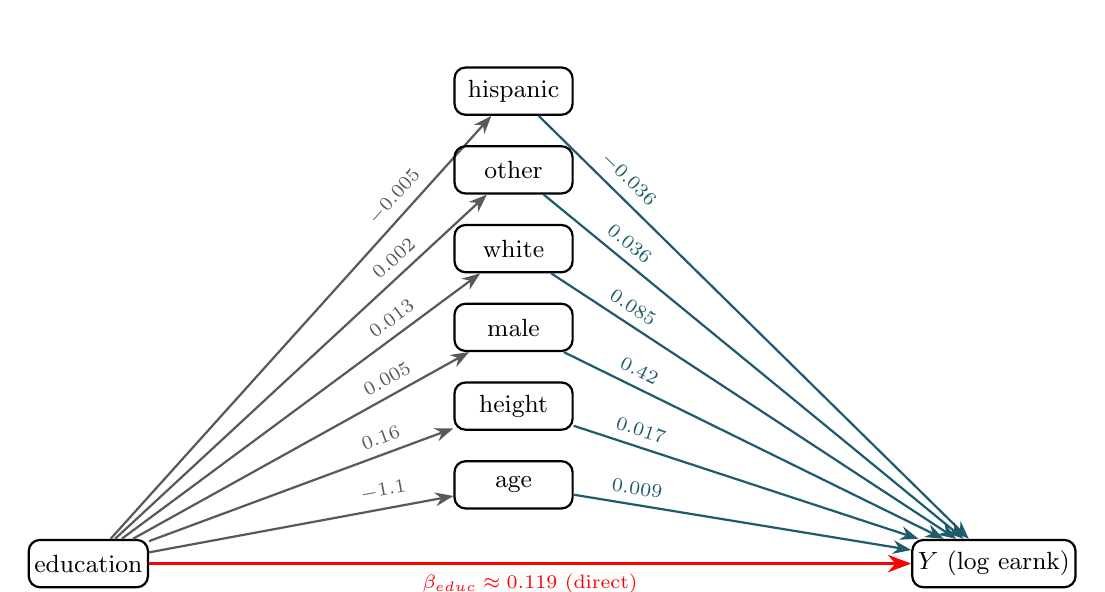
\begin{tikzpicture}[>={Stealth}, every node/.style={font=\small},
  var/.style={rounded corners, draw, thick, minimum height=0.6cm, minimum width=1.5cm, inner sep=2pt}]
\node[var] (E) at (0,0) {education};
\node[var] (Y) at (11.5,0) {$Y$ (log earnk)};
\foreach \n/\y/\lft/\rgt in {hispanic/6.0/{-0.005}/{-0.036}, other/5.0/0.002/0.036, white/4.0/0.013/0.085,
                        male/3.0/0.005/0.42, height/2.0/0.16/0.017, age/1.0/{-1.1}/0.009}{
  \node[var] (\n) at (5.4,\y) {\n};
  \draw[->, thick, gray!70!black] (E) -- node[pos=0.78, above, sloped, font=\scriptsize] {$\lft$} (\n);
  \draw[->, thick, dataclr] (\n) -- node[pos=0.18, above, sloped, font=\scriptsize] {$\rgt$} (Y);
}
\draw[->, very thick, red] (E) -- node[below, font=\scriptsize] {$\beta_{educ}\approx0.119$ (direct)} (Y);
\end{tikzpicture}
\end{center}
\[
\underbrace{0.115}_{\beta'_{educ}}\approx\underbrace{0.119}_{\beta_{educ}}+\underbrace{0.001}_{\text{ethnicity (3 dummies)}}
+\underbrace{0.42\times0.005}_{\text{male}\,\approx\,0.002}+\underbrace{0.017\times0.16}_{\text{height}\,\approx\,0.003}
+\underbrace{0.009\times(-1.1)}_{\text{age}\,\approx\,-0.010}.
\]
(The ethnicity term is $(-0.036)(-0.005)+(0.036)(0.002)+(0.085)(0.013)\approx0.001$.) Reading the arrows: one more year of education goes with
being $0.16$ inches taller and $1.1$ years \emph{younger}, on average. The detours mostly cancel. The only sizable one is age, and it is negative:
age raises earnings, but more-educated people tend to be younger, so leaving age out makes education look slightly \emph{less} valuable.

\textbf{Why are more-educated people younger?} Plotting education and earnings against age, older respondents have less education on
average: they are from earlier generations, when less schooling was typical (the youngest are partly still in school). Earnings rise with age
up to middle age and then level off.

\textbf{Age as a categorical predictor.} Replacing age by one dummy per decade (baseline 18--29; 70 and over pooled), keeping the other
predictors, the scaled age coefficients rise from the 30s to the 40s and then fall in the 50s and 60s. The effect of age is not a straight line,
which the single slope $\beta_{age}$ cannot show. The education coefficient barely changes.

\subsection{Revisiting the elections: past vote only}
\begin{lstlisting}[style=output]
Dep. Variable:                   vote   R-squared:                       0.834
==============================================================================
                 coef    std err          t      P>|t|      [0.025      0.975]
------------------------------------------------------------------------------
const          0.0382      0.012      3.311      0.001       0.016       0.061
past_vote      0.9182      0.020     46.584      0.000       0.879       0.957
\end{lstlisting}
With past vote alone the slope is $0.92$, versus $0.53$ in the model with the two incumbency dummies. The left-out predictors are $X_{dem}$ and
$X_{rep}$; their slopes on past vote are $\beta_{past,dem}\approx2.13$ and $\beta_{past,rep}\approx-1.99$ (a district with 10 points higher past
vote is about 21 points more likely to have a Democratic incumbent, and about 20 points less likely to have a Republican one).
\begin{center}
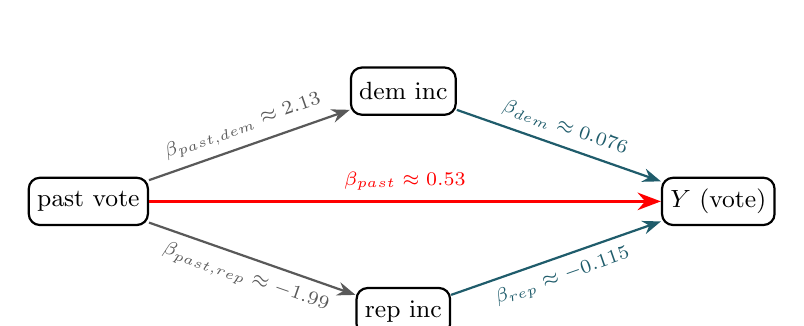
\begin{tikzpicture}[>={Stealth}, every node/.style={font=\small},
  var/.style={rounded corners, draw, thick, minimum height=0.6cm, inner sep=3pt}]
\node[var] (P) at (0,0) {past vote};
\node[var] (Y) at (8,0) {$Y$ (vote)};
\node[var] (D) at (4,1.4) {dem inc};
\node[var] (R) at (4,-1.4) {rep inc};
\draw[->, thick, gray!70!black] (P) -- node[above, sloped, font=\scriptsize] {$\beta_{past,dem}\approx2.13$} (D);
\draw[->, thick, gray!70!black] (P) -- node[below, sloped, font=\scriptsize] {$\beta_{past,rep}\approx-1.99$} (R);
\draw[->, thick, dataclr] (D) -- node[above, sloped, font=\scriptsize] {$\beta_{dem}\approx0.076$} (Y);
\draw[->, thick, dataclr] (R) -- node[below, sloped, font=\scriptsize] {$\beta_{rep}\approx-0.115$} (Y);
\draw[->, very thick, red] (P) -- node[above, font=\scriptsize] {$\beta_{past}\approx0.53$} (Y);
\end{tikzpicture}
\end{center}
\[
\underbrace{0.92}_{\beta'_{past}}\approx\underbrace{0.53}_{\beta_{past}}+\underbrace{0.076\times2.13}_{\beta_{dem}\beta_{past,dem}\,\approx\,0.16}
+\underbrace{(-0.115)\times(-1.99)}_{\beta_{rep}\beta_{past,rep}\,\approx\,0.23}.
\]
Both detours are positive. Districts with a high past vote tend to have Democratic incumbents (who add vote) and not Republican incumbents
(who would subtract vote). Without the dummies, past vote gets credit for the incumbency advantage.

\subsection{Revisiting children's test scores: mother's age}
Add $X_{age}$ (\py{mom\_age}), the mother's age when the child was born.
\begin{lstlisting}[style=output]
Dep. Variable:              kid_score   R-squared:                       0.008
==============================================================================
                 coef    std err          t      P>|t|      [0.025      0.975]
------------------------------------------------------------------------------
const         70.9569      8.307      8.542      0.000      54.631      87.283
mom_age        0.6952      0.362      1.920      0.055      -0.016       1.407
\end{lstlisting}
\begin{lstlisting}[style=output]
Dep. Variable:              kid_score   R-squared:                       0.215
==============================================================================
                 coef    std err          t      P>|t|      [0.025      0.975]
------------------------------------------------------------------------------
const         20.9847      9.130      2.298      0.022       3.039      38.930
mom_hs         5.6472      2.258      2.501      0.013       1.210      10.085
mom_iq         0.5625      0.061      9.276      0.000       0.443       0.682
mom_age        0.2248      0.331      0.680      0.497      -0.425       0.875
\end{lstlisting}
And the single-predictor fits of the other two predictors on mother's age:
\begin{center}
\begin{tabular}{@{}lccc@{}}
\toprule
response & slope on \py{mom\_age} (se) & 95\% CI & $R^2$\\\midrule
\py{mom\_hs} & $\hat\beta_{age,hs}=0.0326$ ($0.007$) & $[0.019,0.047]$ & 0.046\\
\py{mom\_iq} & $\hat\beta_{age,iq}=0.5087$ ($0.266$) & $[-0.014,1.032]$ & 0.008\\
\bottomrule
\end{tabular}
\end{center}

\begin{examplebox}[title={Question (10/21): interpret mom age; why does adding it change so little?}]
\textbf{Interpret.} \emph{Alone:} each extra year of the mother's age goes with $0.70$ more points on average ($p=0.055$; the CI just includes 0,
so the evidence is weak). \emph{With mom hs and mom iq:} comparing mothers with the same schooling and IQ, each year goes with only $0.22$
points, with a CI $[-0.43,0.88]$ that contains 0. There is no evidence of an association once schooling and IQ are controlled for.

\textbf{Why so little changes.} Without age, the coefficients were $5.95$ and $0.564$ with $R^2=0.214$; with age they are $5.65$ and $0.5625$
with $R^2=0.215$. By OVB, the change in another predictor's coefficient from leaving out age is $\beta_{age}$ times how much age moves with that
predictor. Here $\beta_{age}$ is small ($0.22$), and age is only weakly associated with the other predictors ($R^2$ of $0.05$ and $0.01$ above), so
the changes are tiny. Age carries almost no information about the score beyond what schooling and IQ already provide.

\textbf{OVB for the single slope.} Leaving out both hs and iq:
\[
\underbrace{0.70}_{\beta'_{age}}\approx\underbrace{0.22}_{\beta_{age}}+\underbrace{0.0326\times5.65}_{\beta_{age,hs}\beta_{hs}\,\approx\,0.18}
+\underbrace{0.509\times0.5625}_{\beta_{age,iq}\beta_{iq}\,\approx\,0.29}\quad(=0.695).
\]
Most of the single-predictor association runs through schooling and IQ: older mothers are a bit more likely to have finished high school and
have slightly higher IQs, and those are what go with higher scores.
\end{examplebox}
\begin{center}
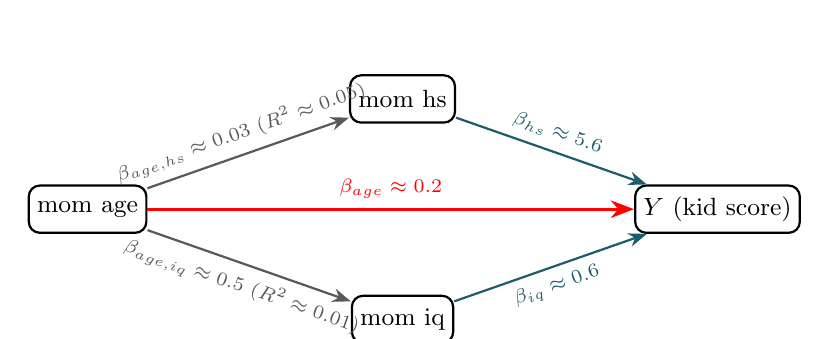
\begin{tikzpicture}[>={Stealth}, every node/.style={font=\small},
  var/.style={rounded corners, draw, thick, minimum height=0.6cm, inner sep=3pt}]
\node[var] (A) at (0,0) {mom age};
\node[var] (Y) at (8,0) {$Y$ (kid score)};
\node[var] (H) at (4,1.4) {mom hs};
\node[var] (I) at (4,-1.4) {mom iq};
\draw[->, thick, gray!70!black] (A) -- node[above, sloped, font=\scriptsize] {$\beta_{age,hs}\approx0.03$ ($R^2\approx0.05$)} (H);
\draw[->, thick, gray!70!black] (A) -- node[below, sloped, font=\scriptsize] {$\beta_{age,iq}\approx0.5$ ($R^2\approx0.01$)} (I);
\draw[->, thick, dataclr] (H) -- node[above, sloped, font=\scriptsize] {$\beta_{hs}\approx5.6$} (Y);
\draw[->, thick, dataclr] (I) -- node[below, sloped, font=\scriptsize] {$\beta_{iq}\approx0.6$} (Y);
\draw[->, very thick, red] (A) -- node[above, font=\scriptsize] {$\beta_{age}\approx0.2$} (Y);
\end{tikzpicture}
\end{center}

%==========================================================
\section{Correlated predictors and the sample distribution (Lecture 16, Unit 4.3--4.4)}\label{sec:collin}
%==========================================================
\subsection{Example: body fat, weight, and hip size}
Percent body fat (from underwater weighing) of 252 men, with weight (lb) and hip circumference (cm). Each predictor alone is strongly
correlated with body fat ($r=0.61$ for weight, $0.63$ for hip), but weight and hip are even more correlated with each other: $r=0.94$.
\begin{center}
\begin{tabular}{@{}lcccc@{}}
\toprule
model & weight coef (se) & hip coef (se) & $p$ (weight) & $R^2$\\\midrule
weight only & $0.1744$ ($0.014$) & --- & $<0.001$ & 0.375\\
hip only & --- & $0.7303$ ($0.058$) & --- & 0.391\\
both & $0.0600$ ($0.041$) & $0.4988$ ($0.170$) & $0.149$ & 0.396\\
\bottomrule
\end{tabular}
\end{center}

\begin{examplebox}[title={Question (10/21): why does the se of weight triple, and weight stop being significant?}]
Weight and hip size are nearly collinear ($r=0.94$): heavier men almost always have bigger hips. In the two-predictor model the data must
separate ``more weight, same hips'' from ``bigger hips, same weight'', and there are few men who differ in one but not the other. Many
combinations of the two coefficients fit almost equally well, so each one is poorly determined. The se of weight goes $0.014\to0.041$ (ratio
$2.9$) and the se of hip $0.058\to0.170$ (ratio $2.9$). That is exactly $1/\sqrt{1-0.94^2}=1/\sqrt{0.116}\approx2.9$ (keybox below).
With $\hat T=0.060/0.041=1.45$, weight is no longer significant, and $R^2$ barely rises ($0.391\to0.396$): weight adds little beyond hip.
The weight coefficient also shrinks, $0.174\to0.060$, by OVB (alone, weight gets credit for hip size).
\end{examplebox}

\begin{keybox}[title={Adding predictors inflates the standard error}]
Let $R_j^2$ be the $R^2$ from regressing $X_j$ on the added predictors. Adding them multiplies the standard error of $\hat\beta_j$ by about
\[
\frac{\se(\hat\beta_j)\ \text{with the others}}{\se(\hat\beta_j)\ \text{alone}}\approx\frac{1}{\sqrt{1-R_j^2}},
\]
times a factor $\hat\sigma_\epsilon(\text{with})/\hat\sigma_\epsilon(\text{alone})\le1$ if the added predictors also explain $Y$. With one added
predictor, $R_j^2=\rho_{1,2}^2$ (derived below).
\inwords{the more the other predictors can predict $X_j$, the less independent information about $X_j$'s effect is left, and the wider its CI.}
\end{keybox}
\begin{figure}[h]
\centering
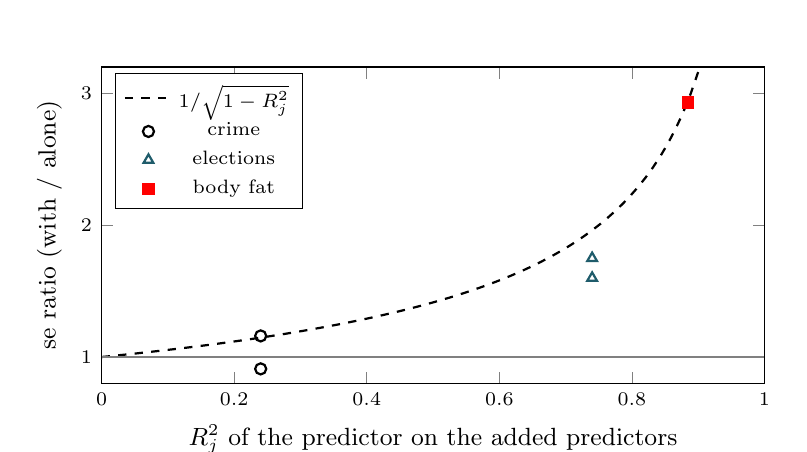
\begin{tikzpicture}
\begin{axis}[width=10cm, height=5.6cm, xmin=0, xmax=1, ymin=0.8, ymax=3.2, xlabel={$R_j^2$ of the predictor on the added predictors},
  ylabel={se ratio (with / alone)}, tick label style={font=\scriptsize}, label style={font=\small},
  legend style={font=\scriptsize, at={(0.02,0.98)}, anchor=north west}]
\addplot[black, dashed, thick, domain=0:0.9, samples=80] {1/sqrt(1-x)};
\addplot[only marks, mark=o, thick] coordinates {(0.24,0.91) (0.24,1.16)};
\addplot[only marks, mark=triangle, thick, dataclr] coordinates {(0.74,1.75) (0.74,1.60)};
\addplot[only marks, mark=square*, red] coordinates {(0.884,2.93) (0.884,2.93)};
\addplot[gray] coordinates {(0,1) (1,1)};
\legend{$1/\sqrt{1-R_j^2}$, crime, elections, body fat}
\end{axis}
\end{tikzpicture}
\caption{Each point is one coefficient from these notes: its se with the other predictor divided by its se alone (crime: Section~\ref{sec:ovb};
elections: below; body fat: above). The se grows when the added predictor is correlated with $X_j$ (body fat, elections); when it is not, the
ratio stays near 1. Points fall a little below the curve because $\hat\sigma_\epsilon$ shrinks.}
\end{figure}

\subsection{The covariance system for two predictors (Unit 4.3)}
Take $Y=\beta_1X_1+\beta_2X_2+\epsilon$ with mean-zero predictors and no intercept. Exactly as in the OVB proof, covariance with each predictor gives
\begin{align*}
\Cov(X_1,Y)&=\beta_1\sigma_{X_1}^2+\beta_2\Cov(X_1,X_2),\\
\Cov(X_2,Y)&=\beta_1\Cov(X_1,X_2)+\beta_2\sigma_{X_2}^2.
\end{align*}
Dividing the first by $\sigma_{X_1}^2$ is the OVB formula $\beta'_1=\beta_1+\beta_2\beta_{1,2}$. In matrix form, with the \textbf{covariance matrix} $\Sigma$:
\[
\begin{bmatrix}\Cov(X_1,Y)\\\Cov(X_2,Y)\end{bmatrix}=\Sigma\begin{bmatrix}\beta_1\\\beta_2\end{bmatrix},\qquad
\Sigma=\begin{bmatrix}\sigma_{X_1}^2&\Cov(X_1,X_2)\\\Cov(X_1,X_2)&\sigma_{X_2}^2\end{bmatrix},
\]
\[
\Sigma^{-1}=\frac{1}{\sigma_{X_1}^2\sigma_{X_2}^2-\Cov(X_1,X_2)^2}\begin{bmatrix}\sigma_{X_2}^2&-\Cov(X_1,X_2)\\-\Cov(X_1,X_2)&\sigma_{X_1}^2\end{bmatrix}.
\]
(For a $2\times2$ matrix $\begin{bmatrix}a&b\\b&d\end{bmatrix}$ the inverse is $\frac{1}{ad-b^2}\begin{bmatrix}d&-b\\-b&a\end{bmatrix}$: swap the diagonal, negate
the off-diagonal, divide by $ad-b^2$.) Solving, $\beta=\Sigma^{-1}\big(\Cov(X_1,Y),\Cov(X_2,Y)\big)$:
\[
\beta_1=\frac{\Cov(X_1,Y)\,\sigma_{X_2}^2-\Cov(X_2,Y)\Cov(X_1,X_2)}{\sigma_{X_1}^2\sigma_{X_2}^2-\Cov(X_1,X_2)^2}
\ \overset{\text{standardized}}{=}\ \frac{\rho_1-\rho_{1,2}\,\rho_2}{1-\rho_{1,2}^2},
\]
where $\rho_k=\corr(X_k,Y)$ and $\rho_{1,2}=\corr(X_1,X_2)$. If the predictors are uncorrelated ($\rho_{1,2}=0$), $\beta_1=\rho_1$: the
single-predictor slope. This compares with $\beta'_1=\Cov(X,Y)/\Var(X)$: $\Sigma^{-1}$ plays the role of $1/\Var(X)$. In practice the same
formula with sample covariances gives the least squares estimates (what \py{sm.OLS} computes).

\subsection{Why correlated predictors are hard to separate}
Take two \emph{standardized} predictors with correlation $\rho_{1,2}$, $Y=\beta_1X_1+\beta_2X_2+\epsilon$. With one predictor,
$\se(\hat\beta_1)=\sigma_\epsilon/(\sigma_X\sqrt N)$. With two, we need the \emph{joint} sample distribution of $(\hat\beta_1,\hat\beta_2)$: how the pair
varies together over replicates.

\textbf{Extreme case, $X_1\approx X_2$.} Then $Y\approx(\beta_1+\beta_2)X_1+\epsilon$. The data pin down the sum $\beta_1+\beta_2$, but not $\beta_1$ and
$\beta_2$ separately: raising $\hat\beta_1$ and lowering $\hat\beta_2$ by the same amount fits almost equally well.

\begin{examplebox}[title={Question (10/21): a new dataset gives a larger $\hat\beta_1$. What do you expect for $\hat\beta_2$?}]
Smaller. The sum $\hat\beta_1+\hat\beta_2$ stays close to $\beta_1+\beta_2$ in every replicate, so when $\hat\beta_1$ comes out high, $\hat\beta_2$ must come out
low to compensate. Across replicates the two estimates are \emph{negatively} correlated: $\corr(\hat\beta_1,\hat\beta_2)=-\rho_{1,2}$ (derived below).
\end{examplebox}

\textbf{The regression plane wobbles.} With two predictors the fitted model is a plane over the $(x_1,x_2)$ plane. If $\rho_{1,2}=0$ the points
cover the plane and fitted planes from different datasets look alike. If $\rho_{1,2}=0.95$ the points lie near the line $x_1=x_2$, so the plane can
tilt about that line without changing the fit much, and fitted planes from different datasets tilt in different directions.

\textbf{Two views (Unit 4.4).} Look at the data along $u=(X_1+X_2)/\sqrt2$ (the direction where the predictors move together) and
$v=(X_1-X_2)/\sqrt2$ (where they disagree). Then
\[
\beta_1X_1+\beta_2X_2=\frac{\beta_1+\beta_2}{\sqrt2}\,u+\frac{\beta_1-\beta_2}{\sqrt2}\,v,\qquad
\Var(u)=1+\rho_{1,2},\quad\Var(v)=1-\rho_{1,2},\quad\Cov(u,v)=0.
\]
($\Var(u)=\frac12(1+1+2\rho_{1,2})$; $\Cov(u,v)=\frac12(\Var X_1-\Var X_2)=0$.) Since $u$ and $v$ are uncorrelated, each slope behaves like a
single-predictor slope, with se $\sigma_\epsilon/(\sigma\sqrt N)$ for that direction's SD $\sigma$. For $\rho_{1,2}$ near 1 the data are spread out along $u$, so the sum
$\beta_1+\beta_2$ is well determined. They are bunched up in $v$ ($\Var v\approx0$), so the difference $\beta_1-\beta_2$ is not. For $\rho_{1,2}$ near $-1$
it is the other way around; for $\rho_{1,2}=0$ the two views look the same.

\begin{keybox}[title={Sample distribution with two predictors}]
If the covariance matrix $\Sigma$ of the predictors is known, the pair $(\hat\beta_1,\hat\beta_2)$ is (approximately) jointly Normal around the truth,
with variances and covariance given by
\[
\begin{bmatrix}\Var(\hat\beta_1)&\Cov(\hat\beta_1,\hat\beta_2)\\\Cov(\hat\beta_1,\hat\beta_2)&\Var(\hat\beta_2)\end{bmatrix}=\frac{\sigma_\epsilon^2}{N}\,\Sigma^{-1}.
\]
For standardized predictors, $\Sigma=\begin{bmatrix}1&\rho_{1,2}\\\rho_{1,2}&1\end{bmatrix}$ and $\Sigma^{-1}=\dfrac{1}{1-\rho_{1,2}^2}\begin{bmatrix}1&-\rho_{1,2}\\-\rho_{1,2}&1\end{bmatrix}$, so
\[
\se(\hat\beta_1)=\frac{\sigma_\epsilon}{\sqrt{N(1-\rho_{1,2}^2)}},\qquad
\corr(\hat\beta_1,\hat\beta_2)=\frac{-\rho_{1,2}/(1-\rho_{1,2}^2)}{1/(1-\rho_{1,2}^2)}=-\rho_{1,2},
\]
\[
\se(\hat\beta_1+\hat\beta_2)=\sigma_\epsilon\sqrt{\frac{2}{N(1+\rho_{1,2})}}.
\]
With $\Sigma=1$ (one standardized predictor) this is the old $\se=\sigma_\epsilon/\sqrt N$. For unstandardized $X_1$, $\se(\hat\beta_1)=\sigma_\epsilon/\big(\sigma_{X_1}\sqrt{N(1-\rho_{1,2}^2)}\big)$.
\inwords{correlated predictors make each coefficient less precise by $1/\sqrt{1-\rho_{1,2}^2}$ and make the two estimates move in opposite directions; their sum stays precise.}
\end{keybox}
For the sum: $\Var(\hat\beta_1+\hat\beta_2)=\Var\hat\beta_1+\Var\hat\beta_2+2\Cov=\frac{\sigma_\epsilon^2}{N}\cdot\frac{2-2\rho_{1,2}}{1-\rho_{1,2}^2}=\frac{2\sigma_\epsilon^2}{N(1+\rho_{1,2})}$
(using $1-\rho^2=(1-\rho)(1+\rho)$). It gets \emph{smaller} as $\rho_{1,2}\to1$.

\begin{figure}[h]
\centering
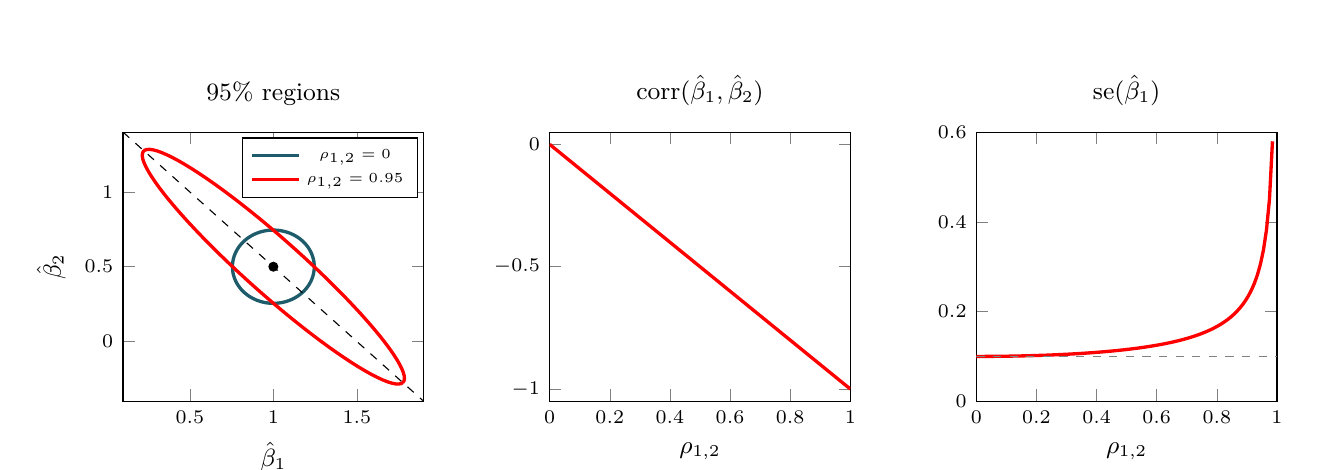
\begin{tikzpicture}
\begin{groupplot}[group style={group size=3 by 1, horizontal sep=1.6cm}, width=5.4cm, height=5cm,
  tick label style={font=\scriptsize}, label style={font=\small}, title style={font=\small}]
\nextgroupplot[xmin=0.1, xmax=1.9, ymin=-0.4, ymax=1.4, xlabel={$\hat\beta_1$}, ylabel={$\hat\beta_2$}, title={95\% regions},
  legend style={font=\tiny, at={(0.98,0.98)}, anchor=north east}]
\addplot[dataclr, very thick, domain=0:360, samples=90] ({1+0.245*cos(x)}, {0.5+0.245*sin(x)});
\addplot[red, very thick, domain=0:360, samples=90] ({1+(1.096*cos(x)+0.175*sin(x))/sqrt(2)}, {0.5+(-1.096*cos(x)+0.175*sin(x))/sqrt(2)});
\addplot[black, dashed, domain=0.1:1.9] {1.5-x};
\addplot[only marks, mark=*, mark size=1.6pt] coordinates {(1,0.5)};
\legend{$\rho_{1,2}=0$, $\rho_{1,2}=0.95$}
\nextgroupplot[xmin=0, xmax=1, ymin=-1.05, ymax=0.05, xlabel={$\rho_{1,2}$}, title={$\corr(\hat\beta_1,\hat\beta_2)$}]
\addplot[red, very thick, domain=0:1] {-x};
\nextgroupplot[xmin=0, xmax=1, ymin=0, ymax=0.6, xlabel={$\rho_{1,2}$}, title={$\se(\hat\beta_1)$}]
\addplot[red, very thick, domain=0:0.985, samples=100] {1/sqrt(100*(1-x^2))};
\addplot[gray, dashed] coordinates {(0,0.1) (1,0.1)};
\end{groupplot}
\end{tikzpicture}
\caption{The slides' simulation model $Y=X_1+0.5X_2+\epsilon$, $\sigma_\epsilon=1$, $N=100$, drawn from the formulas. Left: the regions holding about
95\% of the estimates $(\hat\beta_1,\hat\beta_2)$ over replicates; the dot is the truth $(1,0.5)$ and the dashed line is $\hat\beta_1+\hat\beta_2=1.5$. With
$\rho_{1,2}=0.95$ the cloud stretches along that line. Middle and right: the correlation of the estimates is $-\rho_{1,2}$, and the se grows like
$1/\sqrt{1-\rho_{1,2}^2}$. At $\rho_{1,2}=0.95$, $\se(\hat\beta_1)=1/\sqrt{100\times0.0975}=0.32$, about 3 times the $0.10$ at $\rho_{1,2}=0$, but
$\se(\hat\beta_1+\hat\beta_2)=\sqrt{2/195}=0.10$ is even smaller than the $\sqrt{2/100}=0.14$ at $\rho_{1,2}=0$.}
\end{figure}

\subsection{Real example: incumbency and past vote}
In the election data, $\corr(\text{past vote},\text{inc})=0.86$: incumbents mostly hold districts that already voted for their party.
\begin{center}
\begin{tabular}{@{}lccc@{}}
\toprule
 & inc only & past vote only & both\\\midrule
$\hat\beta_{inc}$ (se) & 0.191 (0.004) & --- & 0.096 (0.007)\\
$\hat\beta_{past}$ (se) & --- & 0.918 (0.020) & 0.521 (0.032)\\
\bottomrule
\end{tabular}
\end{center}
In the model with both, the estimated $\corr(\hat\beta_{past},\hat\beta_{inc})=-0.86$, exactly $-\rho_{1,2}$.

\begin{examplebox}[title={Question (10/21): why are both se's larger with both predictors? Why would a world of safe seats be a problem?}]
\textbf{Larger se's.} The two predictors are strongly correlated, so the data contain few districts where incumbency and past vote disagree,
and those are the only districts that separate the two effects. The inflation factor is $1/\sqrt{1-0.86^2}=1/\sqrt{0.26}\approx1.96$; the observed
ratios are $0.007/0.004\approx1.75$ (inc) and $0.032/0.020=1.6$ (past). They are a bit smaller because $\hat\sigma_\epsilon$ also drops when the second
predictor is added ($R^2$ goes up to $0.887$).

\textbf{Safe seats.} If almost every incumbent held a safe seat (Democratic incumbents only in strongly Democratic districts, and so on), inc
would be almost a function of past vote: $\rho_{1,2}\approx1$. Then $1/\sqrt{1-\rho_{1,2}^2}$ blows up, and the data could not tell whether a high vote
comes from the district's past or from the incumbent. Only the combined effect would be estimable. The districts that identify the incumbency
advantage are the open seats and the ones where the incumbent's party and the district's lean disagree.
\end{examplebox}

%==========================================================
% Formula sheet
%==========================================================
\clearpage
\newgeometry{margin=0.4in}
\begin{landscape}
\pagestyle{empty}
\newcommand{\csh}[1]{\par\vspace{5pt}{\color{accent}\bfseries #1}\vspace{-1pt}\par{\color{accent}\hrule height 0.6pt}\vspace{2pt}\par}
\newtcolorbox{cbox}{colback=tipbg, colframe=orange!70!black, boxrule=0.5pt, arc=1.5pt,
  left=3pt, right=3pt, top=2pt, bottom=2pt, before skip=3pt, after skip=3pt, before upper=\raggedright}
\begingroup
\scriptsize
\setlength{\parskip}{2.5pt}
\setlength{\tabcolsep}{4pt}
{\Large\bfseries\color{accent} Math 50 Midterm 2 \textperiodcentered\ Formula sheet}\hfill{\small Lectures 8--16 \textperiodcentered\ Unit 2.4, Unit 3, Unit 4}\par
{\color{accent}\hrule height 1pt}\vspace{2pt}
\begin{multicols}{4}
\raggedright

\csh{Algebra}
$\Var(aX+b)=a^2\Var X$; independent: $\Var(X\pm Y)=\Var X+\Var Y$.\\
$\Cov(X,Y)=\E[XY]-\E X\E Y$; $\Cov(X,aY+bZ+c)=a\Cov(X,Y)+b\Cov(X,Z)$.\\
iid mean: $\E\Ybar=\mu$, $\Var\Ybar=\sigma^2/N$. \ $\sum_i(Y_i-\Ybar)=0$.\\
$\Bin(N,q)$: mean $Nq$, var $Nq(1-q)$.

\csh{Correlation (2.4)}
$\rho=\dfrac{\beta_1\sigma_X}{\sigma_Y}=\dfrac{\Cov(X,Y)}{\sigma_X\sigma_Y}$ = slope of $Z_Y$ on $Z_X$.\\
$\sigma_Y^2=\beta_1^2\sigma_X^2+\sigma_\epsilon^2$; \ $1-\rho^2=\dfrac{\sigma_\epsilon^2}{\sigma_Y^2}=\dfrac{\Var(Y\given X)}{\Var Y}$.\\
$\rho^2$ = fraction of variance explained, in $[0,1]$.

\csh{LLN / CLT (3.1)}
$S_N/N\to\E X_i$. \ $S_N\approx\Norm(N\mu,N\sigma^2)$, $\ \Ybar\approx\Norm(\mu,\sigma^2/N)$ (iid, finite variance).

\csh{Estimators (3.2)}
$\hat\theta$ random, $\theta$ fixed. Sample distribution = distribution of $\hat\theta$ over replicates; $\se(\hat\theta)$ = its SD.\\
Normal mean: $\hat\mu\sim\Norm(\mu,\sigma^2/N)$, $\se=\sigma/\sqrt N$ ($\hat\sigma/\sqrt N$ in practice).\\
Bernoulli: $\hat q\approx\Norm(q,q(1-q)/N)$.
\begin{cbox}
$\MSE=\E[(\hat\theta-\theta)^2]=\se^2+\Bias^2$, $\ \Bias=\E\hat\theta-\theta$.\\
Unbiased: $\Bias=0$ for all $N$. Consistent: $\E\hat\theta\to\theta$, $\se\to0$.
\end{cbox}
Laplace $\hat q_L=\frac{S+1}{N+2}$: bias $\frac{1-2q}{N+2}$, var $\frac{Nq(1-q)}{(N+2)^2}$.\\
$\hat\sigma_0^2=\frac1N\sum(Y_i-\Ybar)^2$: $\E=\frac{N-1}N\sigma^2$. Bessel: $\hat\sigma^2=\frac1{N-1}\sum(Y_i-\Ybar)^2$ unbiased.\\
Key identity: $\sum(Y_i-\Ybar)^2=\sum(Y_i-\mu)^2-N(\Ybar-\mu)^2$.


\columnbreak
\csh{CIs and tests (3.3, 3.6)}
\begin{cbox}
95\% CI: $\hat\theta\pm1.96\,\se(\hat\theta)$ \ ($t$: 2.78/2.26/2.05 for $N$=5/10/30).\\
$\hat T=\hat\beta_1/\se(\hat\beta_1)$; \ $p_v=\P(|\hat T^*|>|\hat T|)=2(1-\Phi(|\hat T|))$.
\end{cbox}
CI meaning: over replicates, 95\% of CIs contain $\theta$ (not ``95\% chance for this interval'').\\
CI excludes 0 $\iff|\hat T|>1.96\iff p_v<0.05$.\\
Width $\propto1/\sqrt N$: $N\ge(1.96\sigma/\text{half-width})^2$.\\
Binary $X$, $N/2$ per group: $\hat\beta_1\sim\Norm(\beta_1,4\sigma_\epsilon^2/N)$; unequal groups: $\Var=\sigma_\epsilon^2(\frac1{N_0}+\frac1{N_1})$.\\
Density of $Z$ near 0 $\approx0.4$: $\P(|Z|<a)\approx0.8a$ for small $a$.\\
$\hat T^2=(N-2)\dfrac{R^2}{1-R^2}$: small $R^2$ \& tiny $p_v$ possible (big $N$); big $R^2$ \& big $p_v$ impossible.

\csh{Least squares (3.4)}
$\hat\beta_1=\dfrac{\sum(X_i-\Xbar)(Y_i-\Ybar)}{\sum(X_i-\Xbar)^2}$, \ $\hat\beta_0=\Ybar-\hat\beta_1\Xbar$ (minimize SSR).\\
$r_i=Y_i-\hat\beta_0-\hat\beta_1X_i$, \ $\SSR=\sum r_i^2$, \ $\SST=\sum(Y_i-\Ybar)^2$.\\
$\hat\sigma_\epsilon^2=\SSR/(N-2)$, \ $R^2=1-\SSR/\SST$.
\begin{cbox}
Conditional on $X$: $\E\hat\beta_1=\beta_1$;\\
$\hat\beta_1\approx\Norm\!\Big(\beta_1,\dfrac{\sigma_\epsilon^2}{N\sigma_X^2}\Big)$, \ $\se\approx\dfrac{\sigma_\epsilon}{\sigma_X\sqrt N}$.
\end{cbox}
\py{np.cov(x,y)[0,1]/np.cov(x,y)[0,0]} $=\hat\beta_1$.\\
\py{2*(1-norm.cdf(np.abs(T)))} $=p_v$.


\csh{AR(1) (3.5)}
$Y_t=\beta_0+\rho Y_{t-1}+\epsilon_t$; stationary: $\beta_1=\rho$, $\beta_0=(1-\rho)\mu$,\\
$Y_t-\mu=\rho(Y_{t-1}-\mu)+\epsilon_t$, \ $\sigma_Y^2=\dfrac{\sigma_\epsilon^2}{1-\rho^2}$.\\
Autocorrelation $\rho_k=\rho^k$ (exponential decay).\\
Random walk ($\rho=1$): $Y_t\sim\Norm(0,\sigma_\epsilon^2t)$; forecast $Y_t\pm1.96\hat\sigma_\epsilon\sqrt h$.\\
Hurwicz: $\E\hat\rho\approx\rho-2\rho/N$ (biased down, consistent) because $\epsilon_t$ is part of later predictors.\\
Log random walk $\Rightarrow P_{t+1}\approx P_t(1+\epsilon_{t+1})$ (multiplicative).

\csh{Multiple predictors (4.1--4.2)}
RCT: $X$ independent of confounders. Cohort: not.\\
$Y=\beta_0+\beta_1X_1+\beta_2X_2+\epsilon$: $\beta_1$ = effect of $X_1$ with $X_2$ held fixed.\\
Compare predictors with $\hat\beta_k\sigma_{X_k}$.\\
$R^2$ never decreases with more predictors; $R^2$'s do not add.
\begin{cbox}
\textbf{OVB:} $\beta'_1=\beta_1+\beta_2\beta_{1,2}$, \ $\beta_{1,2}=\dfrac{\Cov(X_1,X_2)}{\Var X_1}$\\
(slope of $X_2$ on $X_1$; binary $X_1$: difference of means of $X_2$).
\end{cbox}
$\beta_{1,2}\,\beta_{2,1}=\rho_{12}^2$.\\
Simpson's paradox = OVB with a confounder strong enough to flip the sign.\\
AR(1) on two lags: $\beta_{lag1}=\rho$, $\beta_{lag2}=0$; on lag $k$ alone: $\rho^k$.\\
AR(2) $0.5,0.3$ on lag 1 alone: $\rho_1=0.5+0.3\rho_1\Rightarrow\rho_1=5/7$.

\csh{Many predictors, categorical (4.5)}
\begin{cbox}
$\beta'_1=\beta_1+\sum_{j\ge2}\beta_j\beta_{1,j}$ \ (slides: $\beta'_{1,j}$) = sum over all paths $X_1\to Y$.
\end{cbox}
$m$ categories $\to$ $m-1$ dummies; coef = category $-$ baseline (others fixed).\\
Category $a$ vs.\ $b$: $\beta_a-\beta_b$. All $m$ + intercept: collinear.\\
Linear $X_{inc}\in\{-1,0,1\}$ = dummies with $\beta_{dem}=-\beta_{rep}=\beta_{inc}$.\\
Log response: coef $b$ $\Rightarrow$ $Y\times e^b\approx(1+b)$.

\columnbreak
\csh{Collinearity (4.3--4.4)}
$\Sigma\beta=(\Cov(X_1,Y),\Cov(X_2,Y))$; $\begin{bmatrix}a&b\\b&d\end{bmatrix}^{-1}=\frac{1}{ad-b^2}\begin{bmatrix}d&-b\\-b&a\end{bmatrix}$.\\
Standardized: $\beta_1=\dfrac{\rho_1-\rho_{1,2}\rho_2}{1-\rho_{1,2}^2}$.
\begin{cbox}
$\Var/\Cov$ of $(\hat\beta_1,\hat\beta_2)=\frac{\sigma_\epsilon^2}{N}\Sigma^{-1}$; standardized:\\
$\se(\hat\beta_1)=\dfrac{\sigma_\epsilon}{\sqrt{N(1-\rho_{1,2}^2)}}$, \ $\corr(\hat\beta_1,\hat\beta_2)=-\rho_{1,2}$,\\
$\se(\hat\beta_1+\hat\beta_2)=\sigma_\epsilon\sqrt{2/(N(1+\rho_{1,2}))}$.
\end{cbox}
se inflation $\approx1/\sqrt{1-R_j^2}$. \ $u=\frac{X_1+X_2}{\sqrt2}$: $\Var=1+\rho$; $v$: $1-\rho$.

\csh{Worked numbers}
Graders: $\se\approx1.2$--$1.36$, $\hat T\approx0.4$, $p_v\approx0.7$.\\
Test scores: $11.8=5.95+0.56\times10.3$; scaled $2.4$ vs.\ $8.4$.\\
Jeter: $-0.006+0.067\times0.670=0.039$.\\
Crime: $\hat\beta_{pov,single}=0.565$, $\hat\rho=0.49$.\\
Incumbency: $0.19=0.096+0.52\times0.18$; scaled $0.104$ vs.\ $0.092$.\\
Past vote: $0.92\approx0.53+0.076(2.13)+(-0.115)(-1.99)$.\\
Education: $0.115\approx0.119+0.001+0.002+0.003-0.010$.\\
Mom age: $0.70\approx0.22+0.03(5.6)+0.5(0.56)$.\\
Body fat: $r=0.94$, se $\times1/\sqrt{1-0.94^2}=2.9$.

\csh{Symbol key (full glossary: p.~\pageref{sec:glossary})}
$\hat\theta$ estimate from data \ $\Ybar$ sample average \ $\beta'$ coefficient with the predictor alone\\
$Y\given X$ ``$Y$ given $X$'' \ $\sim$ ``is distributed as'' \ $\sum_i$ add over data points\\
$\approx$ approximately \ $\Rightarrow$ implies \ $\E$ expected value (true average)\\
var / cov / se: variance / covariance / standard error \ $\rho$ correlation\\
$\beta_{1,2}$ slope of $X_2$ regressed on $X_1$ \ $\sigma_\epsilon$ spread around the line

\end{multicols}
\endgroup
\end{landscape}
\restoregeometry

\end{document}
